\documentclass[spanish,a4paper,12pt,twoside,openright]{extreport}

\usepackage[dvips]{graphicx}
\usepackage[dvips]{epsfig}
\usepackage[utf8]{inputenc}
\usepackage[spanish]{babel}
\usepackage{alltt}

\usepackage[ruled,vlined,commentsnumbered,linesnumbered,inoutnumbered,titlenotnumbered,noend]{algorithm2e}
\SetKwRepeat{Do}{do}{while}

\usepackage{multirow}
\usepackage{adjustbox}
\usepackage{array} 
\usepackage{amsfonts}
\usepackage{amsmath}
\usepackage{bigstrut}
\usepackage{booktabs}
\usepackage{caption}
\usepackage{chngpage}
\usepackage{float}
\usepackage{lipsum}
\usepackage{graphicx}
\usepackage{lscape}
\usepackage{microtype}
\usepackage[numbers]{natbib}
\usepackage{pdflscape}
\usepackage{rotating}
\usepackage{subcaption}
\usepackage{ctable}
\usepackage{enumerate}
\usepackage{gensymb}
\usepackage{eurosym}
\usepackage{xcolor}
\usepackage{tabu}
\usepackage{lineno}
\usepackage{hyperref}
\usepackage[top=2cm, bottom=2cm, left=2cm, right=2cm]{geometry}

\newenvironment{sourcecode}
{\begin{list}{}{\setlength{\leftmargin}{1em}}\item\scriptsize\bfseries}
{\end{list}}

\newenvironment{littlesourcecode}
{\begin{list}{}{\setlength{\leftmargin}{1em}}\item\tiny\bfseries}
{\end{list}}

\newenvironment{abstract_en}
{\par\noindent\begin{center}\textbf{Abstract}\end{center}\begin{itshape}\par\noindent}
{\end{itshape}}

\newenvironment{keywords}
{\begin{list}{}{\setlength{\leftmargin}{1em}}\item[\hskip\labelsep \bfseries Keywords:]}
{\end{list}}

\newenvironment{palabrasClave}
{\begin{list}{}{\setlength{\leftmargin}{1em}}\item[\hskip\labelsep \bfseries Palabras clave:]}
{\end{list}}

\usepackage{bera}% optional: just to have a nice mono-spaced font
\usepackage{listings}
\usepackage{xcolor}

\colorlet{punct}{red!60!black}
\definecolor{background}{HTML}{EEEEEE}
\definecolor{delim}{RGB}{20,105,176}
\colorlet{numb}{magenta!60!black}

\lstdefinelanguage{Csharp}{
  morekeywords = {public, private, class, using, void, var, this, get, set, new, if, else, foreach, in, bool, int, string, float, double, static, return, true, false},
  morecomment = [l]{//},
  morecomment = [s]{/}{/},
  morestring = [b]",
  sensitive = true
}

\lstdefinestyle{basicStyle}{
  basicstyle=\ttfamily\color{black},
  commentstyle=\color{black},
  tabsize=2
}

\lstset{
  language=[Sharp]C,
  basicstyle=\ttfamily\small,
  commentstyle=\color{green},
  keywordstyle=\color{blue},
  stringstyle=\color{red},
  tabsize=2,
  columns=fixed,
  breaklines=true,
  frame=none,
  showstringspaces=false,
  showspaces=false,
  showtabs=false,
  xleftmargin=20pt,
  framexleftmargin=20pt,
  framexrightmargin=5pt,
  framexbottommargin=4pt,
  showstringspaces=false
}

\begin{document}

\renewcommand\listtablename{Índice de Tablas}    
\renewcommand\listfigurename{Índice de Figuras}    

%%%%%%%%%%%%%%%%%%%%%%%%%%%%%%%%%%%%%%%%%%%%%%%%%%%%%%%%%%
% Cover page
%%%%%%%%%%%%%%%%%%%%%%%%%%%%%%%%%%%%%%%%%%%%%%%%%%%%%%%%%%
\pagestyle{empty}
\thispagestyle{empty}


\newcommand{\HRule}{\rule{\linewidth}{1mm}}
\setlength{\parindent}{0mm}
\setlength{\parskip}{0mm}

\vspace*{\stretch{0.5}}

\begin{center}

\includegraphics[scale=0.8]{figures/escuela-ingenieria-tecnologia-original}\\[10mm]
{\Huge Trabajo de Fin de Grado}
\end{center}

\HRule
\begin{flushright}
        {\Huge Control de dispositivos electromecánicos mediante un BCI} \\[2.5mm]
        {\Large \textit{Control of Electromechanical Devices using BCI}} \\[5mm]
        {\Large Anabel Díaz Labrador} \\[5mm]


\end{flushright}
\HRule
\vspace*{\stretch{2}}
\begin{center}
  \Large La Laguna, \today
\end{center}

\setlength{\parindent}{5mm}

%%%%%%%%%%%%%%%%%%%%%%%%%%%%%%%%%%%%%%%%%%%%%%%%%%%%%%%%%%
% Signature page (add the official stamp)
%%%%%%%%%%%%%%%%%%%%%%%%%%%%%%%%%%%%%%%%%%%%%%%%%%%%%%%%%%
\newpage
\thispagestyle{empty}

%TODO poner departamento
D. {\bf José Ignacio Estévez Damas}, con N.I.F. 43.786.097-P profesor Titular de Universidad adscrito al Departamento de Ingenier\'ia Inform\'atica y de Sistemas de la Universidad de La Laguna, como tutor


\bigskip
\bigskip
{\bf C E R T I F I C A}

\bigskip
\bigskip
Que la presente memoria titulada:

\bigskip
''{\it Control de dispositivos electromec\'anicos mediante una interfaz cerebro computador}''

\bigskip
\bigskip
\bigskip

\noindent ha sido realizada bajo su dirección por D. {\bf Anabel D\'iaz Labrador},
con N.I.F. 43.492.425-T.

\bigskip
\bigskip

Y para que así conste, en cumplimiento de la legislación vigente y a los efectos
oportunos firman la presente en La Laguna a \today

%%%%%%%%%%%%%%%%%%%%%%%%%%%%%%%%%%%%%%%%%%%%%%%%%%%%%%%%%%
% Acknowledgments
%%%%%%%%%%%%%%%%%%%%%%%%%%%%%%%%%%%%%%%%%%%%%%%%%%%%%%%%%%
\newpage
\thispagestyle{empty}

{ \flushright

\begin{LARGE}
Agradecimientos
\end{LARGE}

\hspace{3mm}

\begin{large}
En primer lugar, me gustaría agradecer a todas las personas que me han acompañado durante estos años en esta etapa de mi vida, compañeros, familiares y amigos...
\par

\end{large}

}

%%%%%%%%%%%%%%%%%%%%%%%%%%%%%%%%%%%%%%%%%%%%%%%%%%%%%%%%%%
% License
%%%%%%%%%%%%%%%%%%%%%%%%%%%%%%%%%%%%%%%%%%%%%%%%%%%%%%%%%%
\newpage
\thispagestyle{empty}

\bigskip
\begin{LARGE}
Licencia
\end{LARGE}

\bigskip
* Si NO quiere permitir que se compartan las adaptaciones de tu obra y NO quieres permitir usos comerciales de tu obra indica:

\begin{center}

\includegraphics[scale=1.8]{images/by-nc-nd_88x31}\\[5mm]
\end{center}

\begin{large}
© Esta obra está bajo una licencia de Creative Commons Reconocimiento-NoComercial-SinObraDerivada 4.0 Internacional.
\end{large}

\bigskip
\bigskip
\bigskip
* Si quiere permitir que se compartan las adaptaciones de tu obra mientras se comparta de la misma manera y NO quieres permitir usos comerciales de tu obra indica:

\begin{center}

\includegraphics[scale=1.8]{images/by-nc-sa_88x31}\\[5mm]
\end{center}

\begin{large}
© Esta obra está bajo una licencia de Creative Commons Reconocimiento-NoComercial-CompartirIgual 4.0 Internacional.
\end{large}

\bigskip
\bigskip
\bigskip
* Si quiere permitir que se compartan las adaptaciones de tu obra y NO quieres permitir usos comerciales de tu obra indica:

\begin{center}

\includegraphics[scale=1.8]{images/by-nc_88x31}\\[5mm]
\end{center}

\begin{large}
© Esta obra está bajo una licencia de Creative Commons Reconocimiento-NoComercial 4.0 Internacional.
\end{large}

%%%%%%%%%%%%%%%%%%%%%%%%%%%%%%%%%%%%%%%%%%%%%%%%%%%%%%%%
\newpage
\thispagestyle{empty}

\bigskip
*Si NO quiere permitir que se compartan las adaptaciones de tu obra y quieres permitir usos comerciales de tu obra indica:

\begin{center}

\includegraphics[scale=1.8]{images/by-nd_88x31}\\[5mm]
\end{center}

\begin{large}
© Esta obra está bajo una licencia de Creative Commons Reconocimiento-SinObraDerivada 4.0 Internacional.
\end{large}

\bigskip
\bigskip
\bigskip
* Si quiere permitir que se compartan las adaptaciones de tu obra mientras se comparta de la misma manera y quieres permitir usos comerciales de tu obra (licencia de Cultura Libre) indica:

\begin{center}

\includegraphics[scale=1.8]{images/by-sa_88x31}\\[5mm]
\end{center}

\begin{large}
© Esta obra está bajo una licencia de Creative Commons Reconocimiento-CompartirIgual 4.0 Internacional.
\end{large}

\bigskip
\bigskip
\bigskip
* Si quiere permitir que se compartan las adaptaciones de tu obra y quieres permitir usos comerciales de tu obra (licencia de Cultura Libre) indica:

\begin{center}
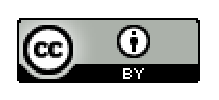
\includegraphics[scale=1.8]{images/by_88x31}\\[5mm]
\end{center}

\begin{large}
© Esta obra está bajo una licencia de Creative Commons Reconocimiento 4.0 Internacional.
\end{large}

%%%%%%%%%%%%%%%%%%%%%%%%%%%%%%%%%%%%%%%%%%%%%%%%%%%%%%%%%%
% Abstract ES
%%%%%%%%%%%%%%%%%%%%%%%%%%%%%%%%%%%%%%%%%%%%%%%%%%%%%%%%%%
\newpage 
\thispagestyle{empty}

\begin{abstract}
{\em

En este trabajo se explora la integración de una interfaz cerebro computador (BCI) para el control de dispositivos electromecánicos. El objetivo principal es explorar y evaluar las aplicaciones beneficiosas de esta interfaz, especialmente en personas con movilidad reducida. Se logró implementar con éxito la interfaz BCI en un sistema Pan-Tilt y un robot móvil. Se llevaron a cabo pruebas con participantes utilizando una interfaz gráfica específicamente desarrollada para evaluar la efectividad y la experiencia de usuario. Los resultados obtenidos indican que el BCI utilizado, NextMind, es una herramienta realmente útil para la inclusión de personas con limitaciones de movilidad, permitiéndoles lograr una mayor independencia en el control de dispositivos electromecánicos específicos, incluida la telepresencia. Además NextMind ha demostrado tener un gran desempeño en ambientes exteriores siendo especialmente útil en el ámbito de control de dispositivos electromecánicos.
}
\bigskip

\begin{palabrasClave}

Interfaz cerebro computador, control de dispositivos electromecánicos, telepresencia, movilidad reducida, inclusión, experiencia de usuario
\end{palabrasClave}

\end{abstract}

%%%%%%%%%%%%%%%%%%%%%%%%%%%%%%%%%%%%%%%%%%%%%%%%%%%%%%%%%%
% Abstract EN
%%%%%%%%%%%%%%%%%%%%%%%%%%%%%%%%%%%%%%%%%%%%%%%%%%%%%%%%%%
\newpage 
\vspace*{200px}
\thispagestyle{empty}

\begin{abstract_en}
{\em

This thesis explores the integration of a brain-computer interface (BCI) for controlling electromechanical devices. The main objective is to investigate and evaluate the beneficial applications of this interface, with a particular focus on individuals with reduced mobility. Successful implementation of the BCI interface was achieved in a pan-tilt system and a robot. Through user testing with a specifically designed graphical interface, effectiveness and user experience were evaluated. The results indicate that brain-computer interfaces are a valuable tool for promoting the inclusion of individuals with mobility limitations, empowering them to achieve greater independence in controlling specific electromechanical devices.
}

\bigskip
\em
\begin {keywords}
Brain-computer interface, electromechanical devices, mobility limitations, inclusion, user experience.
\end {keywords}

\end{abstract_en}

%%%%%%%%%%%%%%%%%%%%%%%%%%%%%%%%%%%%%%%%%%%%%%%%%%%%%%%%%
\newpage{\pagestyle{empty}}
\thispagestyle{empty}

%%%%%%%%%%%%%%%%%%%%%%%%%%%%%%%%%%%%%%%%%%%%%%%%%%%%%%%%%
\pagestyle{myheadings} %my head defined by markboth or markright
% No funciona bien \markboth sin "twoside" en \documentclass, pero al
% ponerlo se dan un montón de errores de underfull \vbox, con lo que no se
% ha puesto.


%%Aqui debería poner el nombre del proyecto pero, como es muy grande no cabe y se ve feo en el PDF
\markboth{xxxxx}{}

%%%%%%%%%%%%%%%%%%%%%%%%%%%%%%%%%%%%%%%%%%%%%%%%%%%%%%%%%
%Numeracion en romanos
\renewcommand{\thepage}{\roman{page}}
\setcounter{page}{1}
\pagestyle{plain} 

%%%%%%%%%%%%%%%%%%%%%%%%%%%%%%%%%%%%%%%%%%%%%%%%%%%%%%%%%

\tableofcontents

%%%%%%%%%%%%%%%%%%%%%%%%%%%%%%%%%%%%%%%%%%%%%%%%%%%%%%%%%
\newpage{\pagestyle{empty}}

\listoffigures

%%%%%%%%%%%%%%%%%%%%%%%%%%%%%%%%%%%%%%%%%%%%%%%%%%%%%%%%%
\newpage{\pagestyle{empty}}

\listoftables

%%%%%%%%%%%%%%%%%%%%%%%%%%%%%%%%%%%%%%%%%%%%%%%%%%%%%%%%%%%%%%%%%%%%%%%%%%%%%%%
\newpage{\pagestyle{empty}}

%%%%%%%%%%%%%%%%%%%%%%%%%%%%%%%%%%%%%%%%%%%%%%%%%%%%%%%%%%%%%%%%%%%%%%%%%%%%%%%
\newpage
\thispagestyle{empty}

%Numeracion a partir del capitulo I
\renewcommand{\thepage}{\arabic{page}}
\setcounter{page}{1}
\pagestyle{plain}

\chapter{\LARGE Introducción}
\label{chapter:introduction}

\section{Contexto y justificación}

Una interfaz cerebro computador (BCI, por sus siglas en inglés) establece una comunicación directa entre la actividad eléctrica del cerebro y dispositivos externos, como ordenadores o dispositivos electromecánicos. Estas interfaces se clasifican en diferentes niveles de invasividad según la proximidad de los electrodos y el tejido cerebral, pudiendo ser no invasivas, parcialmente invasivas o invasivas.

\bigskip

La integración de interfaces cerebro computador en el control de dispositivos presenta numerosas ventajas y aplicaciones. Uno de las ventajas más destacadas es su capacidad para ayudar a personas con problemas de movilidad a realizar tareas cotidianas, como el manejo de una silla de ruedas, el control una prótesis o la interacción con sistemas domóticos.

\bigskip

En el marco del presente Trabajo de Fin de Grado en Ingeniería Informática, se enfoca en el estudio e integración de una interfaz cerebro computador específica, denominada NextMind, para el control dispositivos electromecánicos. 

\bigskip

NextMind, una startup de neurotecnología que ganó el premio a la Mejor Innovación en CES 2020, el 8 de diciembre de 2020, NextMind sacó su kit de desarrollo para su dispositivo BCI llamado por el mismo nombre. \cite{BusinessWire2020} Posteriormente, fue adquirida por Snap Inc, una reconocida empresa de tecnología y cámaras estadounidense. \cite{SnapInc} 

\bigskip

NextMind destaca por su robustez en la detección del estímulo en la actividad cerebral, lo cual lo convierte en una herramienta confiable para la captura precisa de las señales cerebrales. Además, su asequible precio lo hace accesible para investigadores y desarrolladores. Asimismo, su relativa comodidad de uso garantiza una experiencia satisfactoria para los usuarios durante sesiones prolongadas de interacción con el BCI.

\bigskip

Dada la creciente importancia de las interfaces cerebro-computadora en numerosas aplicaciones, el objetivo principal de este trabajo es investigar y desarrollar una aplicación en el que se use NextMind para el control de dispositivos electromecánicos, con el fin de explorar su viabilidad y potencial en esta área.
\section{Objetivos}

Los objetivos del presente trabajo de fin de grado son los siguientes:

\begin{enumerate}
\item Desarrollar una aplicación en Unity que permita la creación de una interfaz de usuario basada en BCI para el control de dispositivos electromecánicos, como por ejemplo un servomotor o un interruptor. Esta aplicación proporcionará las herramientas UI necesarias para la interacción fluida entre el usuario y los dispositivios mediante la detección y el procesamiento de las señales cerebrales.

\item Adaptar la aplicación a un caso de uso concreto, como el control de una silla robotizada o un robot móvil. En el presente objetivo es necesario tener en cuenta las necesidades y requisitos del dispositivo objetivo.

\item Evaluar tanto las ventajas como los inconvenientes de la utilización de interfaces cerebro computador en un caso de uso concreto. En este objetivo recopilarán datos y se realizará un análisis de la experiencia de diferentes usuarios al interactuar con el BCI y los dispositivos electromecánicos controlados. En este se examinan aspectos como la eficacia y la facilidad de uso, con el objeto de identificar mejoras y áreas de futuro desarrollo.
\end{enumerate}
\section{Estado del arte}

El uso de los BCI para el control de dispositivos está ganando popularidad debido a su potencial para mejorar la vida diaria de las personas con movilidad limitada. También aparecen nuevas ideas para su uso habitual, como por ejemplo, siendo parte de la interfaz de usuario en sistemas de realidad virtual (VR) o realidad aumentada (AR). Este proyecto se centra en los métodos que utilizan cascos EEG de tipo malla y, particularmente, en aquellos basados en SSVEP, dada su fiabilidad y alto rendimiento.
Específicamente, se utilizará el dispositivo NextMind, una BCI existente en el mercado que utiliza el enfoque SSVEP. La selección de este dispositivo se basa en su accesibilidad, robustez y comodidad.



Un estudio relevante es ``\textit{Robotic Arm with Brain}'', que utiliza una BCI no invasiva basada en EEG para controlar un brazo robótico \cite{RoboticArmWithBrain} Esta investigación proporciona un marco sobre cómo se pueden utilizar los BCIs para controlar dispositivos físicos de manera efectiva.



Por otra parte, el estudio ``\textit{A New SSVEP based BCI Application on the Mobile Robot in A Maze Game}'', se centra en el desarrollo de un juego de laberinto controlado por una BCI basada en SSVEP con el objetivo de mejorar la calidad de vida de las personas con enfermedad de las neuronas motoras. A la interfaz cerebro-computador se le proporcionan 4 opciones de movimiento:  ``girar en sentido antihorario'', ``girar en sentido horario'', ``desplazarse hacia adelante'' y ``desplazarse hacia atrás''. Para facilitar esas elecciones se utiliza un monitor LCD para mostrar iconos que parpadean a diferentes frecuencias. Esta técnica aprovecha la respuesta de las neuronas en el lóbulo occipital, encargado de procesar los estímulos visuales, que se sincronizan con la frecuencia de la luz percibida por los ojos. Los resultados demostraron que este control basado en SSVEP puede brindar entretenimiento a las personas con dicha enfermedad en el contexto del juego de laberinto.\cite{SSVEPBCIRobotMazeGame} La relación con el presente trabajo radica en el funcionamiento del BCI, que es similar en términos de los estímulos utilizados, así como en las opciones de movimiento proporcionadas.



Finalmente, el estudio ``\textit{A Telepresence Mobile Robot Controlled With a Noninvasive Brain–Computer Interface}'' presenta un sistema de telepresencia basado en EEG que permite a los usuarios tener presencia en entornos remotos a través de un robot móvil con acceso a Internet. El sistema utiliza una BCI basada en el potencial P300 y un robot móvil con capacidades de navegación autónoma y orientación de la cámara \cite{TelepresenceMobileRobotBCI} La relación con el trabajo de fin de grado se encuentra en el concepto de la telepresencia, donde se busca utilizar dispositivos controlados por una interfaz cerebro-computadora para lograr una presencia remota en entornos a través de un robot móvil. En este proyecto, se aplicarán ideas similares para permitir a los usuarios controlar objetos y tener una presencia remota mediante la interfaz cerebro-computadora.



La revisión de los estudios anteriores, especialmente aquellos relacionados con BCIs que utilizan el enfoque SSVEP, ha sido muy útil. En particular, el dispositivo NextMind, que se utiliza en este proyecto, ha proporcionado un marco útil para el diseño y la implementación del estudio.
\section{Metodologías de investigación}
\label{researchmethodology}

Este proyecto adopta una metodología de investigación empírica, implementada a través de pruebas con usuarios. La elección de un diseño empírico se basa en la naturaleza individualizada del uso del casco BCI, que requiere una calibración única para cada individuo. Esta metodología permite analizar las variaciones individuales y determinar su efecto en la calibración y el rendimiento del BCI.



Las pruebas se realizaron con una aplicación que he desarrollado para el control de dispositivos electromecánicos, en este caso un sistema Pan-Tilt con una cámara M5 Stack Timercam.



La aplicación de Pan-Tilt está diseñada para controlar los dos grados de libertad del sistema y ofrecer la visualización en tiempo real del entorno desde la cámara que posee.



Las pruebas para el sistema Pan-Tilt se desarrollaron en un entorno que cuenta con un recorrido de códigos QR dispuestos en distintos planos.



\subsection{Participantes y reclutamiento}

Para este experimento, se reclutaron 16 participantes a través de la universidad y de amigos y conocidos. Se realizó un esfuerzo para asegurar la diversidad de la muestra, lo cual enriquece los resultados al permitir la observación de una gama más amplia de reacciones individuales al BCI. No se proporcionaron incentivos más allá de la oportunidad de experimentar con tecnología innovadora.



\subsection{Procedimiento experimental}

El experimento consta de dos partes principales: la calibración y la prueba. La calibración del BCI se realiza al principio y dura 55 segundos. Este proceso consiste en mostrar una serie de patrones o estímulos visuales a ciertas frecuencias para que el BCI pueda reconocer y calibrarse a las respuestas cerebrales individuales.

Una vez calibrado el BCI, se inicia la prueba, que tiene una duración máxima de diez minutos. Para el control del tiempo se ha incorporado un cronómetro en la aplicación. Los participantes deben recorrer un circuito de códigos QR dispuestos en distintos planos desde el inicio hasta donde puedan llegar o hasta que lo finalicen.

Los experimentos se realizarán en tres condiciones diferentes: sin luz en interior, con luz en interior y con luz en exterior. Este enfoque permite evaluar la funcionalidad de la aplicación en diversas condiciones de iluminación, ya que este factor parece influir en la precisión de la interfaz cerebro computador.



\subsection{Recopilación y análisis de datos}

Durante las pruebas, se lleva un seguimiento de comportamientos inesperados, especialmente en caso de fallos del BCI. También se controlará el tiempo de calibración del BCI, si los participantes finalizan la prueba y, en caso de ser así, el tiempo que les lleva hacerlo.



Los datos recopilados serán analizados a través de medidas descriptivas básicas, incluyendo el promedio. Además, se buscarán posibles correlaciones entre los diferentes factores, como la edad del participante y el tiempo de calibración del BCI.



\subsection{Consideraciones éticas}

En cuanto a la ética en la investigación, se ha garantizado el consentimiento informado, la privacidad y la confidencialidad de los participantes a través del cuestionario anteriormente mencionado que se entregó al final del experimento.



\subsection{Gestión de problemas}

Se espera que existan variaciones en los resultados entre los distintos individuos. No obstante, todas las pruebas se realizan de manera uniforme para mantener la coherencia del experimento. En caso de problemas o fallos en el BCI durante la experimentación, se ha incorporado un sistema de registro de fallos en la aplicación. Este sistema permite al participante registrar un fallo en la aplicación cuando detecte que el BCI ha fallado, proporcionando un registro contable de los problemas encontrados durante la prueba.

%%%%%%%%%%%%%%%%%%%%%%%%%%%%%%%%%%%%%%%%%%%%%%%%%%%%%%%%%%
\newpage{\pagestyle{empty}}
\thispagestyle{empty}

\chapter{\LARGE Marco Teórico}
\label{chapter:theoreticalFramework}

\section{Interfaz cerebro-computador: definición y tecnología}

Los sistemas de interfaces cerebro-computadora surgieron como una respuesta a la necesidad de agregar nuevas formas de interacción más allá de las convencionales, con el objetivo de brindar soluciones diferentes y efectivas. En particular, los BCIs no invasivos son de interés debido a su accesibilidad, seguridad y facilidad de uso, sin necesidad de procedimientos quirúrgicos. La eficacia de estos sistemas se basa en gran medida en su capacidad para detectar y registrar la actividad eléctrica del cerebro, siendo el electroencefalograma (EEG) uno de los métodos más utilizados. Esto conlleva a pagar el precio de obtener señales más pobres con respecto a los métodos invasivos.



En este sentido, los sistemas BCI enfocan su atención en regiones específicas del cerebro, dependiendo de su propósito. Esta especificidad es de particular relevancia en el contexto de la investigación de BCI.

\subsection{Metodologías de BCI basados en EEG}

Hay dos metodologías que se utilizan actualmente: los impulsos cerebrales relacionados con eventos (ERPs, por sus siglas en inglés) y el electroencefalograma oscilatorio (EEG oscillation).



Los ERP son potenciales eléctricos generados por nuestro cerebro en respuesta a diversos eventos, ya sean cognitivos, sensoriales o motores. Estos ERPs actúan como señales eléctricas que nos brindan una visión interna de cómo el cerebro procesa y responde a estímulos específicos.



El segundo grupo de metodologías se basa en el análisis de la actividad oscilatoria del electroencefalograma (EEG). Estas técnicas implican la monitorizaci\'on continua de las diferentes frecuencias presentes en la señal cerebral, como las ondas alfa, beta, gamma, delta y theta, que suelen representar el nivel de consciencia/estrés que posee el individuo\cite{ABHANG201619}. A diferencia de los ERPs, las técnicas basadas en EEG oscilatorio no requieren un estímulo externo predefinido para llevar a cabo el análisis adecuado.



Cabe resaltar que ambas metodologías tienen sus propias ventajas y aplicaciones en el estudio de la actividad cerebral. Los ERPs resultan especialmente útiles en investigaciones cognitivas y en la evaluación de funciones sensoriales - motoras. Por otro lado, los BCIs basados en EEG oscilatorio ofrecen la posibilidad de examinar patrones de actividad cerebral en diferentes frecuencias sin necesidad de un estímulo externo controlado, lo cual facilita su aplicación en contextos más flexibles y naturales.

Dentro de los ERPs se encuentran:

\begin{itemize}
  \item BCIs basados en EEG P300: Estos BCIs miden el potencial evocado P300 que proporciona información valiosa sobre varios procesos cognitivos, como la memoria y la atención \cite{ComparisonAuditoryTemporalLobeEpilepsy}
  
  \item BCIs basados en Potencial Evocado Visual de Estado Estacionario, conocido por sus siglas en inglés SSVEP: Este enfoque detecta las respuestas cerebrales a la estimulación visual a frecuencias específicas y ha ganado popularidad debido a su alto rendimiento y robustez \cite{SSVEPBCI}
\end{itemize}

Dentro de los EEG oscilatorio se encuentra:

\begin{itemize}
  \item BCIs basados en EEG motor imagery (MI-BCI): Las MI-BCIs detectan las señales cerebrales generadas cuando el usuario imagina un movimiento específico. Han mostrado ser útiles en la medicina, particularmente en la rehabilitación motora de personas que han sufrido accidentes cerebrovasculares \cite{MotorImageryRoboticFeedback}
\end{itemize}

Dentro del marco de este Trabajo de fin de grado se usan los BCIs basados en SSVEP.

\subsection{BCIs basados en SSVEP}

Los BCI basados en SSVEP generan una respuesta utilizando frecuencias eléctricas constantes concentradas en el lóbulo occipital ocasionadas por estímulos visuales.



Cuando se encuentra un estímulo visual con una frecuencia específica y registrada por el BCI, las células de la corteza visual se sincronizan y oscilan a la misma frecuencia. Esta sincronización se refleja en la actividad eléctrica del cerebro y se puede medir, como se mencionó anteriormente, utilizando técnicas de electroencefalografía (EEG).
Los BCI basados en SSVEP generalmente registran las fluctuaciones eléctricas producidas por la actividad neuronal, mediante electrodos colocados en el cuero cabelludo. Es importante a destacar es que con este método se añade ruido a los resultados y dependiendo de la persona, por lo que hay que realizar cálculos para contrarrestarlo.




Para capturar de manera eficaz la actividad cerebral, se utilizan estos electrodos y se transmiten a una base de datos. Estos electrodos se suelen agrupar en forma de casco para el usuario. 



Se utilizan varios algoritmos y métodos de procesamiento de señales para extraer la información de SSVEP (Potenciales Evocados Visuales en Estado Estacionario) del ruido de fondo y de las señales cerebrales irrelevantes. Estos incluyen métodos de filtrado espacial, algoritmos de reconocimiento de frecuencia SSVEP y métodos de aprendizaje automático.

\subsection{Diferencias entre BCIs SSVEP y NextMind}

A pesar de que NextMind es bastante reservado sobre el funcionamiento interno de su dispositivo, hay varios aspectos clave que lo diferencian de los BCIs SSVEP tradicionales.

\subsubsection{Arquitectura}

NextMind emplea una arquitectura única que se centra en el lóbulo occipital, una región cerebral responsable de la interpretación de la información visual. A diferencia de otros BCIs que requieren un casco completo para cubrir múltiples regiones cerebrales, NextMind es un dispositivo compacto y liviano que se coloca en la parte posterior de la cabeza, proporcionando una mayor comodidad para el usuario.

\subsubsection{Sistema Híbrido: Inteligencia Artificial}

Una de las características más notables de NextMind es su uso de inteligencia artificial para mejorar la precisión y la eficiencia del dispositivo. NextMind implementa una red neuronal que el usuario debe entrenar inicialmente para que el dispositivo pueda ajustarse mejor a las señales cerebrales específicas del usuario. Este enfoque híbrido facilita una adaptación más personalizada y eficiente a las respuestas cerebrales individuales.

\subsubsection{Patrón de Estímulo}

NextMind emplea un patrón de estímulo novedoso para potenciar la captación de las respuestas visuales. En lugar de los patrones convencionales utilizados en los BCIs SSVEP, NextMind utiliza una malla de puntos, donde cada ``neurotag'' parpadea a una frecuencia específica. Esta innovadora forma de estimulación visual puede ayudar a mejorar la detección y el seguimiento de los estímulos visuales por parte del dispositivo.



Un NeuroTag generalmente consiste en un patrón visual o un objeto en una interfaz gráfica que está diseñado para provocar una respuesta neural específica cuando el usuario lo observa. Estas respuestas neuronales pueden ser registradas y decodificadas por la BCI de NextMind, lo que permite al sistema inferir la intención del usuario a través del monitoreo de las reacciones cerebrales a estos neurotags (véase en la figura \ref{figure:nextmind-neurotag})

\begin{figure}[!htb]
   \centering
    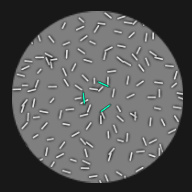
\includegraphics[width=0.4\linewidth]{figures/Neurotag.png}
   \caption{Neurotag de NextMind}
   \label{figure:nextmind-neurotag}
\end{figure}

\subsection{Modulación por Ancho de Pulso (PWM)}
\label{subsection:pwm}

La Modulación por Ancho de Pulso (PWM, por sus siglas en inglés) es una técnica empleada para controlar la cantidad de energía entregada a un dispositivo electrónico mediante la manipulación del ancho de los pulsos en una señal de onda. En este proyecto, esta técnica es esencial para el control preciso del mecanismo Pan-Tilt.



El rango de ciclo de trabajo (duty cycle) para la PWM generalmente va desde 0 a 32767, esto corresponde a una resolución de 15 bits. Sin embargo, en el caso del control de un servomotor, este rango completo puede no ser aprovechado\cite{Espressif2023}



En muchos servomotores, un pulso de 1 milisegundo (ms) se traduce en un ángulo de 0 grados, mientras que un pulso de 2 ms se traduce en un ángulo de 180 grados. Estos pulsos se aplican en un período total de 20 ms, que corresponde a una frecuencia de 50 Hz, comúnmente encontrada en servomotores.



Usando la resolución máxima de 15 bits, el valor del duty cycle para un pulso de 1 ms puede ser calculado de la siguiente manera:

\[
duty_{1ms} = \frac{1ms}{20ms} \times (2^{15} - 1) \approx 1638
\]

Para un pulso de 2 ms, el cálculo es similar:

\[
duty_{2ms} = \frac{2ms}{20ms} \times (2^{15} - 1) \approx 3277
\]



Por ende, para la mayoría de los servomotores, el rango útil de los valores del ciclo de trabajo estaría aproximadamente entre 1638 y 3277. Cabe señalar que este rango puede variar en función de las especificaciones concretas de cada servomotor, por lo que es imprescindible revisar siempre la documentación correspondiente al dispositivo en cuestión. En muchas ocasiones, es útil comprobar de forma empírica cuáles son los límites reales del servomotor.

%%%%%%%%%%%%%%%%%%%%%%%%%%%%%%%%%%%%%%%%%%%%%%%%%%%%%%%%%%

%%%%%%%%%%%%%%%%%%%%%%%%%%%%%%%%%%%%%%%%%%%%%%%%%%%%%%%%%%%%%%%%%%%%%%%%%%%%%%%
\newpage{\pagestyle{empty}}
\thispagestyle{empty}

\chapter{\LARGE Herramientas y tecnologías}
\label{chapter:toolsAndTechnologies}

\section{BCI NextMind}

El BCI NextMind\footnote{NextMind: \url{https://ar.snap.com/welcome-nextmind}} como se ha mencionado anteriormente es una interfaz cerebro-computador revolucionaria. El dispositivo se presenta en forma de un casco compacto y ligero, diseñado y pensado para la comodidad y facilidad de uso del usuario.



El dispositivo NextMind se caracteriza por su diseño inalámbrico, lo que facilita la movilidad y mejora la comodidad del usuario. Este casco viene con una banda ajustable mediante una cinta de velcro, lo que permite adaptarse a diferentes tamaños y formas de cabeza, garantizando así su accesibilidad y funcionalidad para una amplia diversidad de usuarios.



NextMind se distingue por sus nueve electrodos colocados estratégicamente para capturar las señales electroencefalográficas (EEG) desde el lóbulo occipital del cerebro. Estos electrodos registran las respuestas neuronales provenientes de los ``neurotags'' visuales y envía la respuesta a la computadora del usuario (véase en la figura \ref{figure:nextmind-electrodes})

\begin{figure}[!htb]
   \centering
    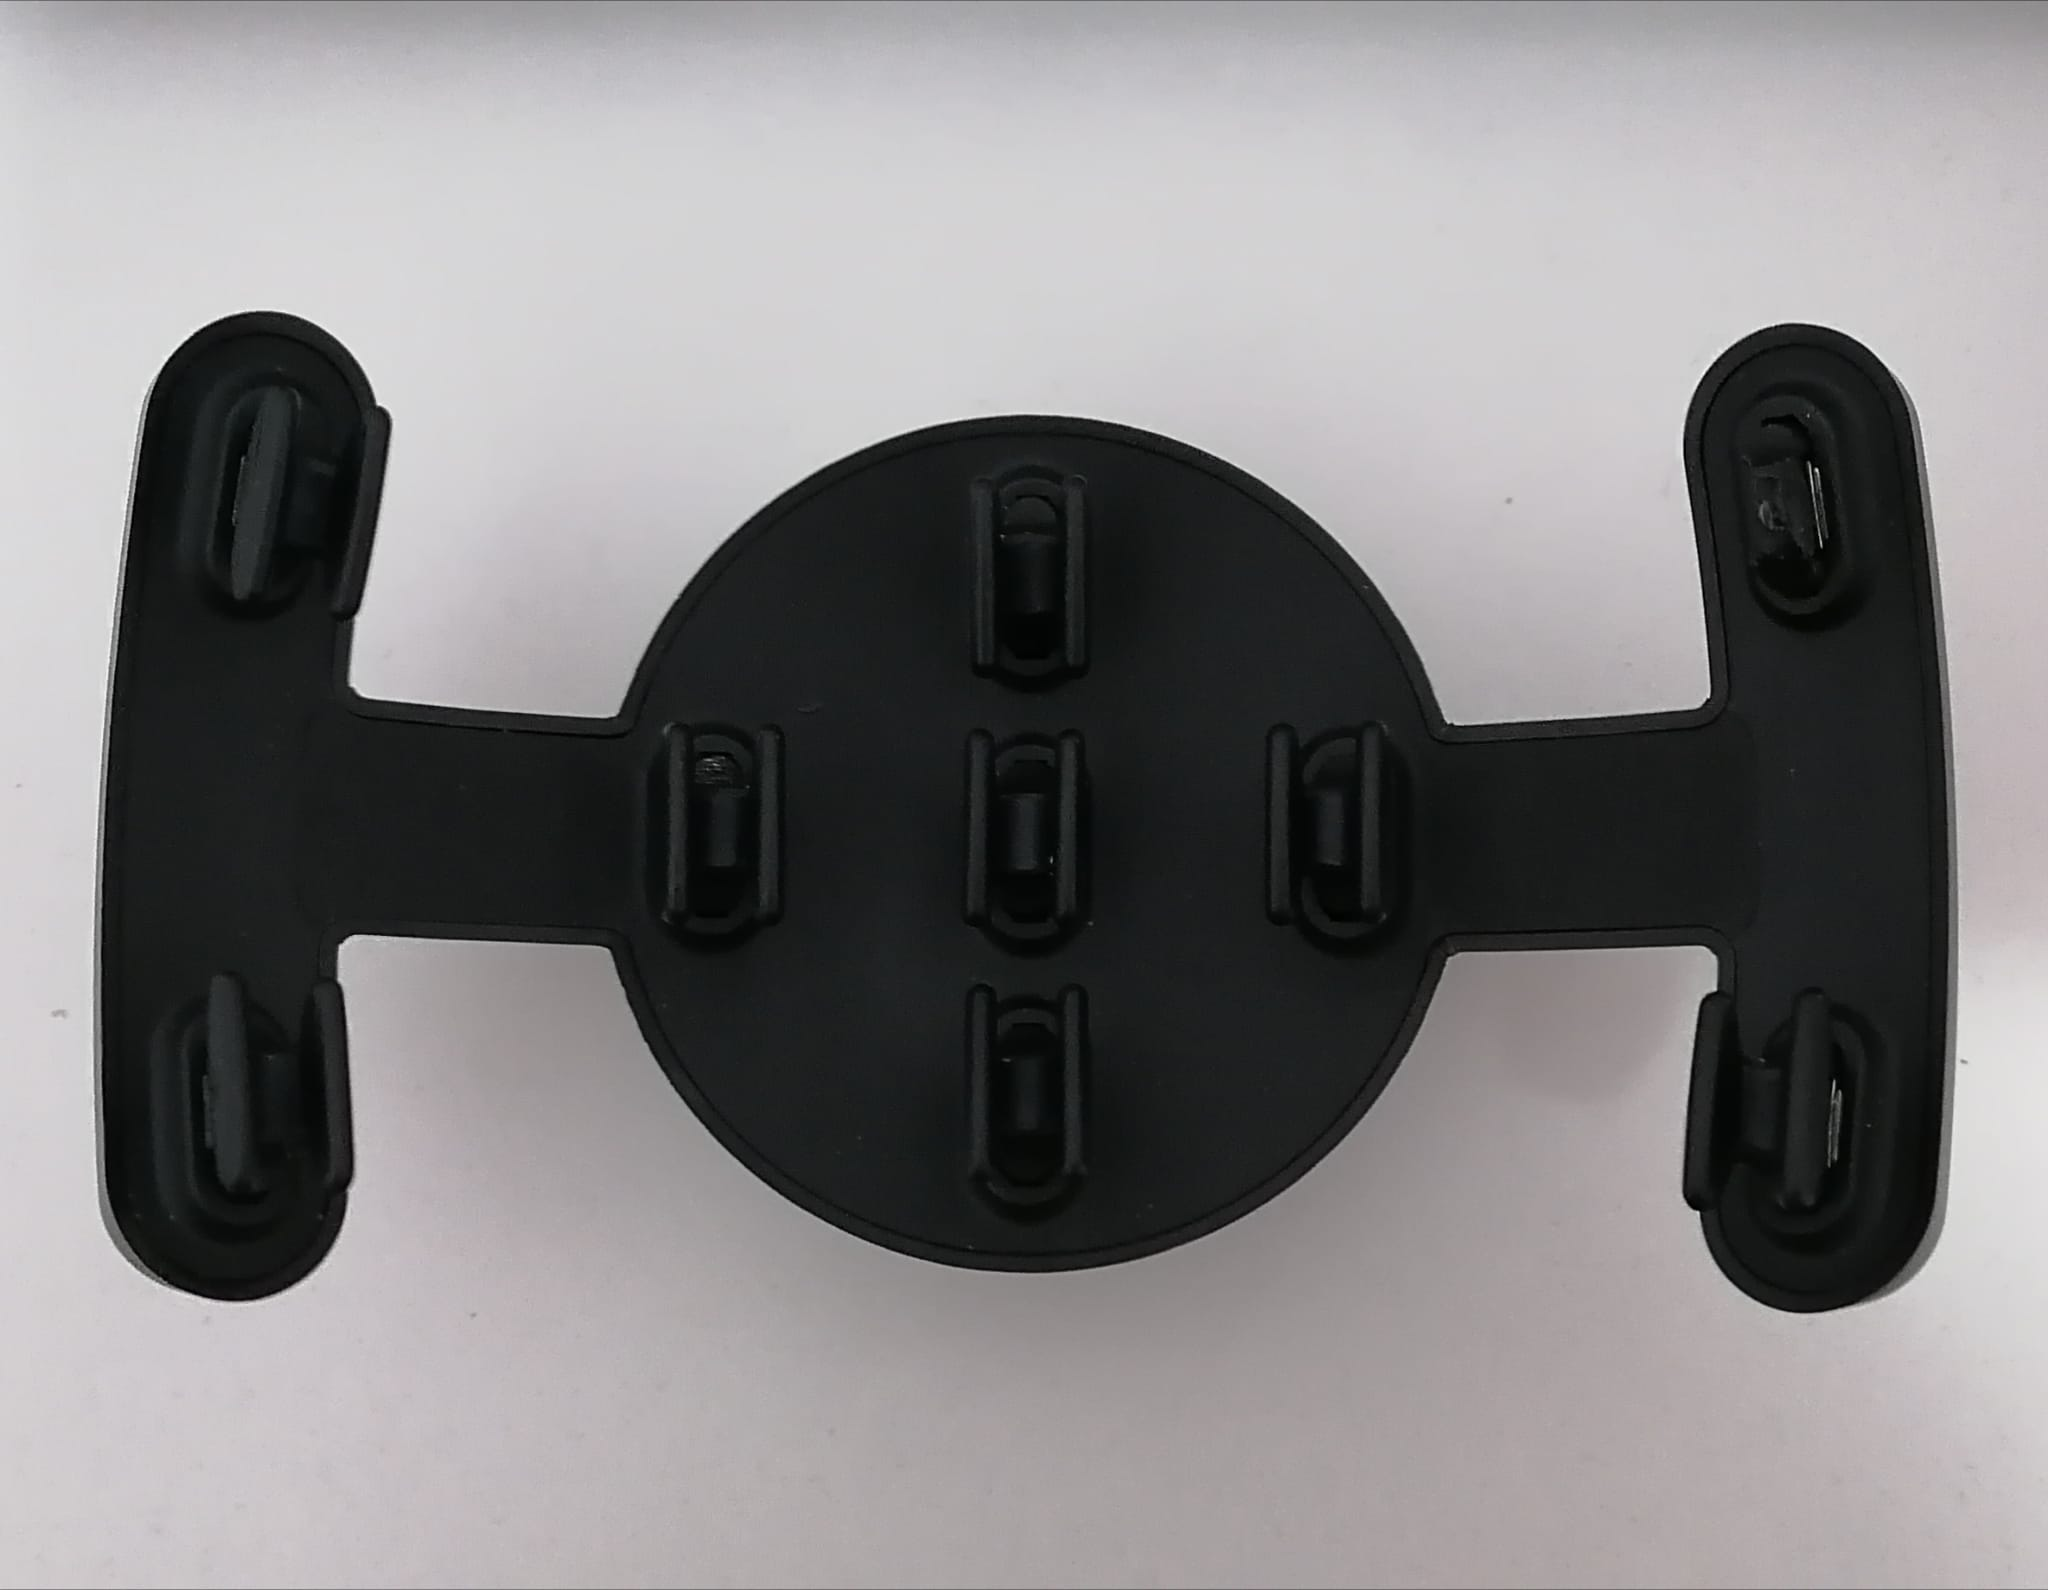
\includegraphics[width=0.5\linewidth]{figures/NextMind electrodes.jpg}
   \caption{Electrodos del casco NextMind}
   \label{figure:nextmind-electrodes}
\end{figure}



Una de las características más relevantes de NextMind es su proceso de encriptación de señales EEG. Al encriptar las señales, NextMind evita que terceros no autorizados puedan interpretar o alterar estas señales. Esta estrategia de encriptación plantea desafíos adicionales en el estudio de de su tecnología, ya que limita la disponibilidad de información detallada sobre su funcionamiento interno.



Estas señales encriptadas son transmitidas vía Bluetooth y sólo pueden ser procesadas a través de la plataforma de desarrollo Unity 3D a través del uso de la SDK proporcionado por el fabricante de NextMind.

\section{Unity 3D}

Unity3D\footnote{Unity3D: \url{https://unity.com/}} es una de las plataformas de desarrollo de videojuegos 3D más importantes del mercado. Esta herramienta polifacética no solo se utiliza en la creación de videojuegos, sino también en la producción de simulaciones, experiencias de realidad virtual (VR) y aumentada (AR), y aplicaciones interactivas para diversas industrias, que podrían ser útiles para su implementación con NextMind.



La plataforma utiliza principalmente los lenguajes de programación C\# y UnityScript, una variante de JavaScript. Ofrece un entorno de desarrollo visual que permite a los creadores diseñar, personalizar y controlar los entornos virtuales y sus interacciones sin necesidad de programar cada detalle desde cero. Unity3D también incluye una extensa biblioteca de activos y herramientas predefinidas para acelerar el proceso de desarrollo.



En el contexto de este Trabajo de Fin de Grado, Unity3D adquiere una importancia especial por su integración con el dispositivo NextMind, siendo esta plataforma la única que el sistema de desarrollo de NextMind permite utilizar.

\section{NextMind SDK}

El SDK de NextMind\footnote{NextMind SDK \url{https://github.com/Snapchat/NextMind/l}} para Unity ofrece un conjunto de herramientas diseñadas para facilitar el desarrollo de juegos y aplicaciones que aprovechan la tecnología NextMind. Este SDK proporciona una API de alto nivel que abstrae a los desarrolladores del funcionamiento interno del BCI. Para el desarrollo de este trabajo, se ha hecho uso extensivo de esta SDK.



El SDK de NextMind se centra principalmente en dos componentes esenciales: el NeuroTag y el NeuroManager.

\subsection{NeuroTags}
\label{subsection:NeuroTags}

El NeuroTag es un componente que permite hacer que cualquier objeto en una aplicación sea interactuable con el BCI. En términos prácticos, los NeuroTags son elementos visuales en la interfaz de usuario que el dispositivo NextMind puede reconocer y seguir. Actualmente, el SDK puede manejar hasta 10 NeuroTags activos simultáneamente, aunque se espera que este número aumente en futuras versiones del SDK. En el marco de este proyecto se utilizaron NeuroTags en la interfaz para que mediante la interacción con esos NeuroTags, se enviara una orden determinada a los dispositivos electromecánicos. Un ejemplo de NeuroTag se puede ver en la Figura \ref{figure:nextmind-neurotag} mostrada anteriormente.

\subsection{NeuroManager}
\label{subsection:NeuroManager}

El NeuroManager es el componente que gestiona la comunicación entre los NeuroTags presentes en la escena y el núcleo del motor de NextMind. Su función es facilitar la coordinación entre los diferentes NeuroTags y el procesamiento de las señales cerebrales captadas por el dispositivo NextMind. Este componente es esencial para cualquier proyecto que utilice NextMind.

\subsection{Otras funcionalidades}

Además de los NeuroTags y el NeuroManager, el SDK de NextMind ofrece una amplia gama de funciones adicionales que pueden ser utilizadas para personalizar las aplicaciones. Estas funciones permiten, por ejemplo, obtener información del sensor de NextMind (como el nivel de batería, el contacto, etc.), gestionar el comportamiento de escaneo de Bluetooth, simular entradas, entre otros. 



El SDK también incluye varios tipos de ``assets'', divididos en dos categorías: los ``assets'' esenciales para construir una aplicación habilitada para NextMind y los ``assets'' de ejemplo que muestran las mejores prácticas para el uso del SDK.



El SDK también incluye varios tipos de ``assets'', divididos en dos categorías:

\begin{itemize}
    \item Assets principales: son todos los archivos esenciales necesarios para crear una aplicación habilitada para NextMind. Encontrará dentro de las librerías principales que exponen las clases principales y algunos activos convenientes (prefabricados, sombreadores, componentes, herramientas, etc.).
    \item Assets de ejemplo: muestra varios ejemplos de cómo usar el SDK, que enseñan las mejores prácticas (por ejemplo, cómo crear su aplicación de calibración personalizada o cómo etiquetar un objeto).
\end{itemize}

Estas características adicionales fueron empleadas en el proyecto para mandar una retroalimentación sobre el estado del casco BCI e implementar una calibración personalizada dentro de la aplicación.
\section{ROS2}
El objetivo de este proyecto es controlar sistemas electromecánicos mediante una interfaz de usuario en un ordenador convencional, haciendo uso de una aplicación distribuida con elementos de cómputo en diversos puntos. Dicha configuración requiere de un medio eficiente para comunicar comandos entre estos elementos, y aquí es donde ROS2\footnote{ROS2 Humble: \url{https://docs.ros.org/en/humble/index.html}} cobra relevancia.



ROS2 es un conjunto de bibliotecas de software y herramientas que permite la creación de aplicaciones distribuidas, comúnmente utilizadas en el control de robots. Esta segunda generación de ROS se ha desarrollado para mantener y expandir las características más útiles de su predecesor, introduciendo al mismo tiempo mejoras significativas en áreas como el rendimiento, la seguridad y el soporte para sistemas embebidos.



La arquitectura de ROS2 es más modular y flexible, permitiendo a los desarrolladores aprovechar y combinar diferentes bibliotecas y herramientas de manera más eficiente. Además, utiliza un modelo de comunicación basado en la publicación y suscripción, lo que facilita una comunicación eficaz entre diferentes dispositivos electromecánicos.



En el contexto de este trabajo, ROS2 es particularmente relevante debido a su capacidad para integrarse con Unity3D a través de librerías como \texttt{ROS2ForUnity} o \texttt{Unity-Robotics-Hub}. De este modo, es posible desarrollar una aplicación en Unity3D que utilice la interacción proporcionada por un BCI para el control de dispositivos robóticos.


\section{MicroROS}

MicroROS\footnote{MicroROS: \url{https://micro.ros.org/}} es una adaptación de ROS2 especialmente diseñada para llevar sus capacidades a sistemas embebidos. Esta herramienta, optimizada para operar con restricciones de recursos de hardware y energía, permite extender el ecosistema de ROS2 a estos sistemas. Con MicroROS, los desarrolladores pueden programar estos sistemas utilizando las mismas herramientas y procedimientos empleados para las máquinas ROS2 más potentes.



Además, MicroROS se integra de manera nativa con ROS2, permitiendo que los sistemas embebidos equipados con MicroROS interactúen con otros sistemas basados en ROS2, comportándose como nodos de ROS2 a través de la ejecución de un agente, aspecto que se explicará más adelante.



En el contexto de este proyecto, MicroROS ofrece la posibilidad de incorporar directamente ROS2 en un microcontrolador, lo que abre la puerta a la manipulación directa del funcionamiento de los sistemas robóticos a nivel de hardware. Esto proporciona una gran flexibilidad y precisión para la implementación de aplicaciones robóticas complejas.
\section{Microcontrolador ESP32}

Para el control efectivo de dispositivos en proyectos como este, la elección de un microcontrolador adecuado es de gran importancia. Es esencial contar con un componente que gestione eficazmente la comunicación entre los diferentes elementos del sistema y que posea la capacidad suficiente para realizar las tareas requeridas sin comprometer el rendimiento. En este sentido, se ha seleccionado el microcontrolador ESP32\footnote{ESP32 \url{https://www.espressif.com/en/products/socs/esp32}}, desarrollado por Espressif Systems, para este proyecto.



El ESP32 es un microcontrolador de alto rendimiento que se ha ganado reconocimiento en el campo de los sistemas embebidos y el Internet de las Cosas (IoT), gracias a su robusto rendimiento, bajo consumo de energía y versatilidad.



En este proyecto, el ESP32 desempeña el papel de microcontrolador principal. Su combinación de potencia y la incorporación del marco de trabajo de MicroROS le permiten ejecutar un nodo de ROS2, convirtiéndolo en un componente clave para el logro de los objetivos del proyecto.


\section{Entorno de desarrollo ESP-IDF}

Para la programación del microcontrolador ESP32 en este proyecto, se ha elegido el entorno de desarrollo ESP-IDF (Espressif IoT Development Framework)\footnote{ESP-IDF \url{https://docs.espressif.com/projects/esp-idf/en/latest/esp32/}}. Esta elección se sustenta en las diversas bibliotecas y herramientas que ESP-IDF proporciona, simplificando la programación de alto rendimiento para estos dispositivos. Además, una característica determinante es su compatibilidad con MicroROS, permitiendo su integración como un componente de ESP-IDF\footnote{Componente microROS \url{https://github.com/micro-ROS/micro_ros_espidf_component/}}.



El ESP-IDF posee un sistema de compilación basado en CMake que permite una configuración del proyecto flexible, la detección automática de dependencias y la compilación cruzada para los microcontroladores ESP32, facilitando el desarrollo del proyecto.


\subsection{Tests: Unity - ThrowTheSwitch}

Para la implementación de pruebas unitarias en el código C del proyecto del microcontrolador, se ha seleccionado Unity - ThrowTheSwitch (U-TTS)\footnote{U-TTS pruebas unitarias para C: \url{https://www.throwtheswitch.org/unity}}, un marco de pruebas para el lenguaje de programación C desarrollado por ThrowTheSwitch.org. Su integración por defecto con los proyectos ESP-IDF asegura una compatibilidad perfecta con el microcontrolador ESP32 utilizado en este proyecto.



U-TTS destaca por su diseño ligero y portátil, lo que lo hace adecuado para proyectos embebidos. Su sintaxis simple facilita su uso y, aunque está diseñado para C, U-TTS puede usarse con casi cualquier lenguaje que se compile a través de C, incluyendo C++. Además, es compatible con una variedad de entornos de compilación y plataformas.



En este proyecto, el uso de U-TTS permite realizar una verificación sistemática de la funcionalidad del código escrito, incrementando la fiabilidad del sistema en desarrollo y facilitando el mantenimiento y la detección temprana de errores.
\section{Pan-Tilt}

Para el control de la orientación de una cámara en este proyecto, se utiliza un sistema Pan-Tilt. Este mecanismo permite ajustar con precisión la dirección en la que la cámara está orientada, ampliando el campo de visión y mejorando la versatilidad del sistema. Los movimientos del sistema Pan-Tilt son controlados a través del microcontrolador ESP32, que gestiona las órdenes provenientes de la interfaz de usuario.



El Pan-Tilt utilizado está construido de forma artesanal y se encontraba en el laboratorio del departamento. Se construyó para un artículo científico llamado en inglés ``A new approach in controlling the motors of a binocular camera head'' \cite{PanTilt2004}. Se ha optado por su uso con la intención de mantener el sistema lo más abierto y adaptable posible.



Este mecanismo está equipado con servomotores HITEC HS-645MG\footnote{HITEC HS-645MG Datasheet \url{https://media.digikey.com/pdf/Data\%20Sheets/Hi-Tech/HS-645MG.pdf}}, que son reconocidos por su alta resistencia, robustez y precisión. Estos servomotores son capaces de mover y mantener de manera precisa la posición de la cámara, a pesar de las vibraciones o las cargas externas (véase la figura \ref{figure:pan-tilt})

\begin{figure}[!htb]
   \centering
    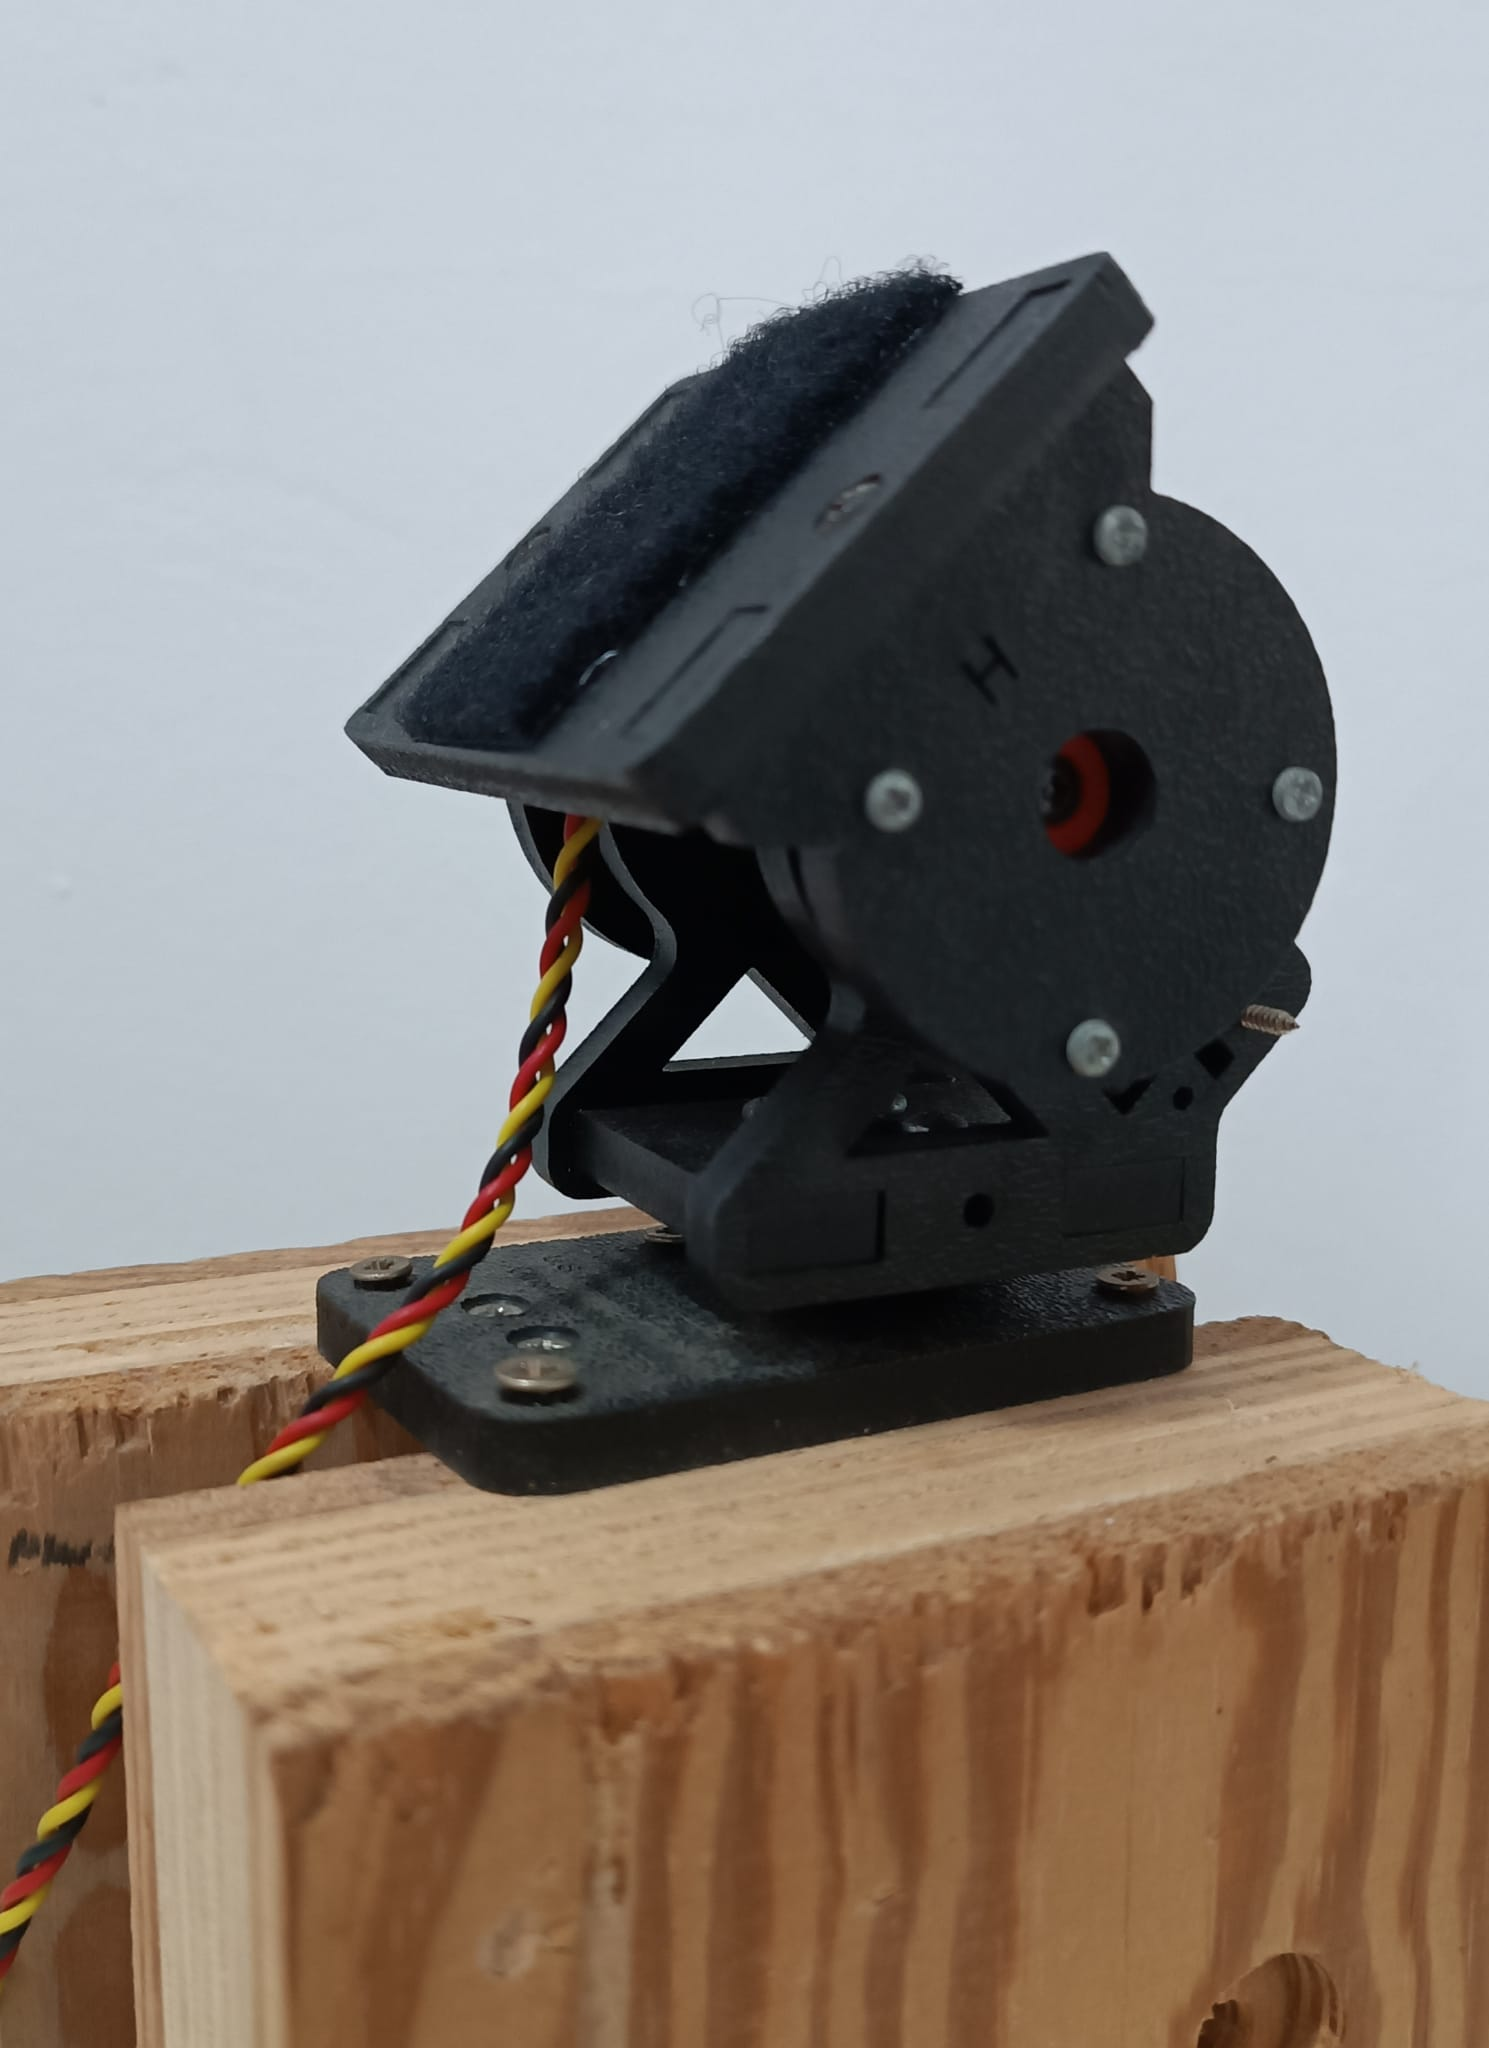
\includegraphics[width=0.3\linewidth]{figures/pan-tilt.jpg}
   \caption{Pan-Tilt artesanal}
   \label{figure:pan-tilt}
\end{figure}
\section{Cámara}
\label{section:camara}

Este proyecto integra una cámara conocida como M5 Stack Timercam \footnote{M5 Stack Timercam \url{https://m5stack.com/products/timercam-m5stack}}, que destaca por su capacidad para realizar streaming de las imágenes captadas vía HTTP. Además, está equipada con un software de detección de códigos QR.

La cámara M5 Stack Timercam es fundamental en este proyecto debido a su capacidad para proporcionar una retroalimentación visual en la interfaz de usuario. El sistema de apuntado se beneficia de un componente que reacciona si se ha logrado un apuntado correcto, permitiendo al usuario percibir de manera clara si están funcionando correctamente sus interacciones con la interfaz (véase la figura \ref{figure:camera})

\begin{figure}[!htb]
   \centering
    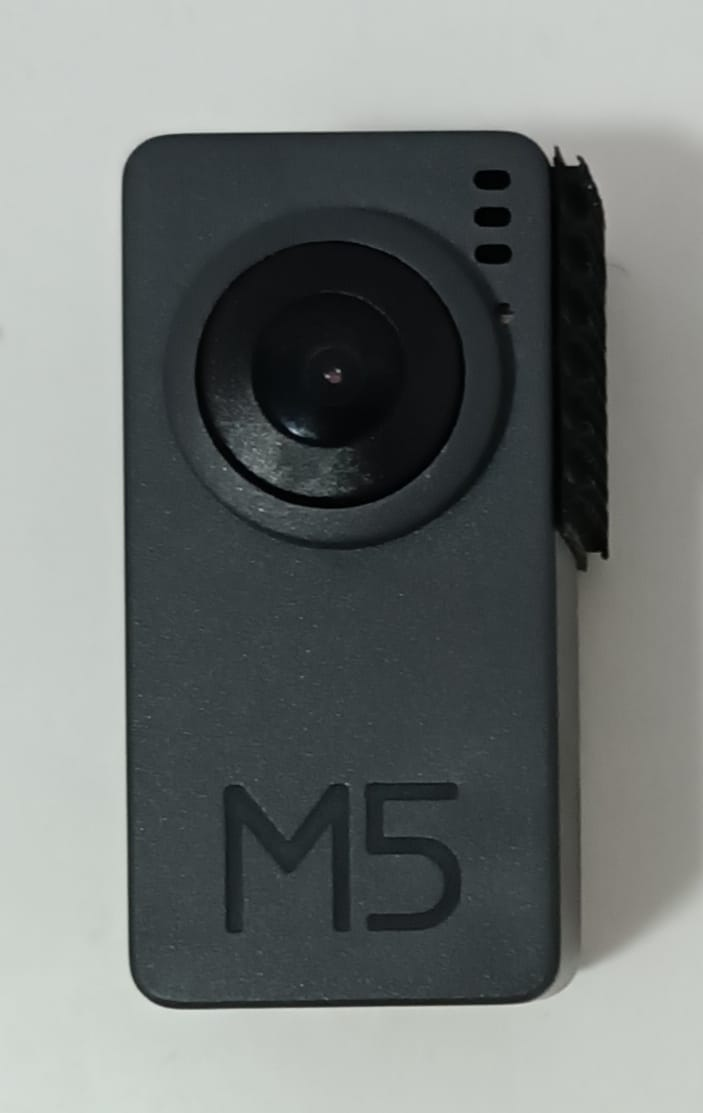
\includegraphics[width=0.25\linewidth]{figures/camera.jpg}
   \caption{Cámara M5 Stack Timercam}
   \label{figure:camera}
\end{figure}



%%%%%%%%%%%%%%%%%%%%%%%%%%%%%%%%%%%%%%%%%%%%%%%%%%%%%%%%%%

\newpage{\pagestyle{empty}}
\thispagestyle{empty}

\chapter{\LARGE Desarrollo del proyecto}
\label{chapter:projectDevelopment}

En este cap\'itulo se describe el desarrollo del proyecto. En primer lugar, se verá el entorno general del proyecto, explicando a grandes rasgos como funciona el proyecto en conjunto. Luego se explica la construcci\'on del interfaz de usuario en Unity, donde interviene de forma directa el sistema de interacci\'on cerebro - computador. A continuaci\'on se describe el desarrollo del sistema controlado, en este caso un Pan - Tilt equipado con una c\'amara. El control del sistema Pan-Tilt implica el desarrollo de una aplicaci\'on ESP-IDF para un ESP32 montado en una targeta de desarrollo. La aplicaci\'on de la c\'amara inteligente no forma parte de este proyecto de fin de grado, por lo que no se describe aqu\'i aunque s'i se enumeran los requisitos que debe cumplir en relaci\'on a las dem\'as partes del proyecto.

\section{Entorno general del proyecto}
\label{section:generalenvironment}

Una vez instalado todo el entorno correctamente (véase , es el momento de explicar cómo se integran todos los componentes para poner en funcionamiento el proyecto.



La figura \ref{figure:diagram-ros2forunity} presenta un diagrama que representa la visión general del sistema.



Es importante mencionar que todos los componentes de ROS 2 deben estar dentro de la misma red. De esta forma, Unity puede conectarse a la red en la que se está ejecutando el agente de micro-ROS. Esta red es generada por el microcontrolador ESP32, que actúa como punto de acceso.



\begin{figure}[!htb]
\centering
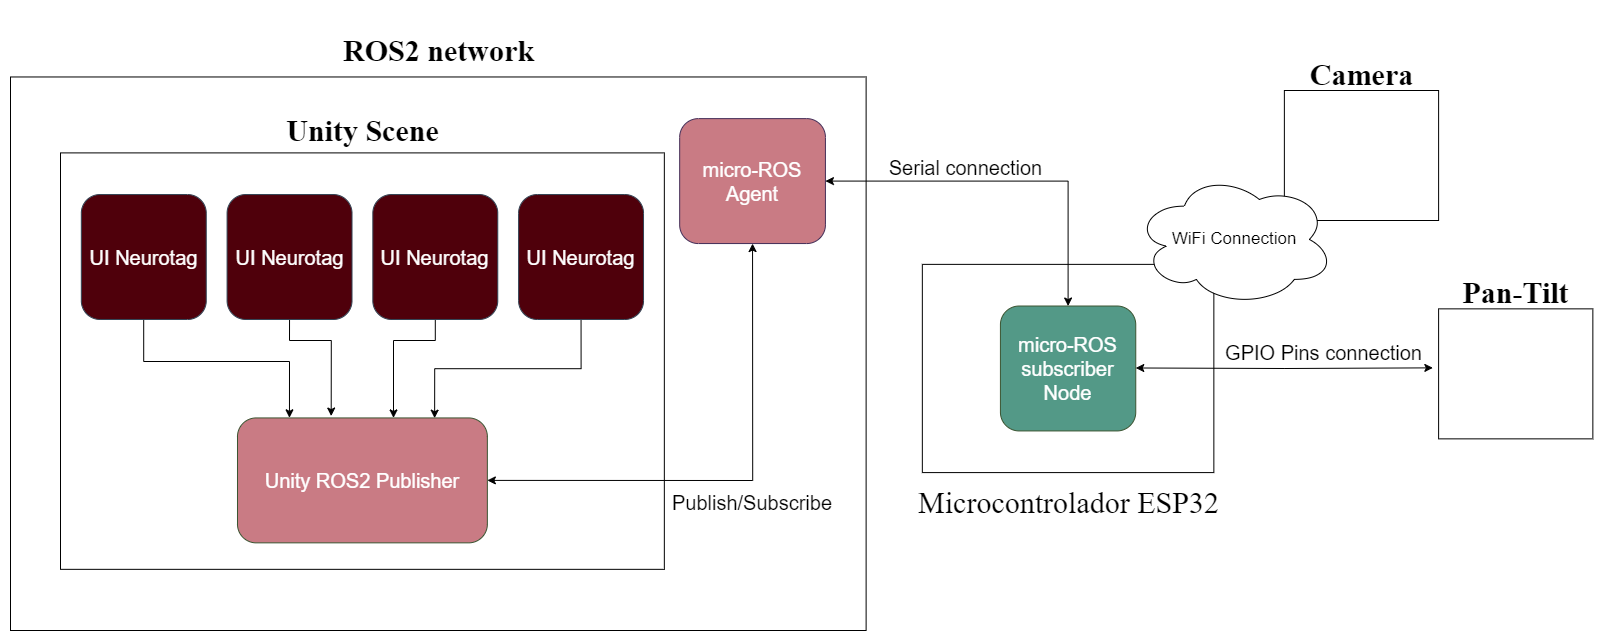
\includegraphics[width=1\linewidth]{figures/Diagram-Ros2ForUnity.png}
\caption{Diagrama del funcionamiento del sistema}
\label{figure:diagram-ros2forunity}
\end{figure}
% Añadir el topic action entre el Publisher y micro-ROS



Con ayuda de la librería Ros2ForUnity, Unity crea un nodo publicador de ROS2 que publica en el tópico ``action''. Un tópico o topic en ROS es un nombre que se utiliza para identificar un canal de comunicación a través del cual los nodos pueden publicar o suscribirse a mensajes.

El nodo suscriptor en el microcontrolador ESP32 se suscribe a este mismo tópico, lo que le permite integrarse en la red de ROS2 a través del agente que se está ejecutando.



Una vez que se ha establecido la comunicación entre Unity y el ESP32, el microcontrolador recibe los mensajes que el nodo publicador transmite a través de ROS2, lo que le permite actuar en consecuencia para controlar el sistema Pan-Tilt y la cámara.



Para garantizar la correcta comunicación, se ha creado un nodo suscriptor en Unity y un nodo publicador en el ESP32 (no representados en el diagrama). Ambos nodos están adscritos al tópico ``freertos\_header\_log'', lo que permite el control de errores. También se ha acabado usando como controlador de la cámara y para que el ESP32 envíe la IP de la cámara a Unity y que este no tenga que saberla de antemano. Gracias a esto Unity no necesita a priori saber su IP sino que será guardada automáticamente cuando la cámara se conecte.

\section{Interfaz de Unity}

En esta sección se explicará la interfaz realizada en Unity para el control de los dispositivos usando Unity y ROS2.

\subsection{Uso de NextMind SDK}

El primer objetivo de este proyecto es explorar el uso del dispositivo NextMind en una interfaz gráfica de usuario bidimensional. Esto es importante, porque los ejemplos proporcionados por NextMind están principalmente basados en objetos 3D, y exist\'ian dudas sobre el correcto funcionamiento del API proporcionada por el fabricante en otros contextos como este.

A continuaci\'on se describe la incorporaci\'on a la aplicaci\'on de diferentes elementos del API de NextMind, que conceptualmente fueron descritos en el cap\'itulo dedicado a la tecnolog\'ia empleada.

\subsubsection{NeuroManager}

Para incorporar el NeuroManager, concepto explicado en el apartado \ref{subsection:NeuroManager}, se emplea un ``prefab''. Los prefabs son componentes prefabricados en Unity que permiten reutilizar configuraciones de objetos. Para incorporar el NeuroManager a la escena simplemente se arrastra el prefab correspondiente.



Es importante recalcar que solo puede existir un único NeuroManager activo en un instante dado. Para garantizar que su persistencia a lo largo de las diferentes escenas y evitar su duplicación, se añadió un script llamado DontDestroyOnLoad. Este script verifica si ya existe una instancia de NeuroManager y, en caso afirmativo, destruye cualquier instancia adicional. Si no existe ninguna instancia previa, mantiene la instancia actual en todas las escenas.



El código del script DontDestroyOnLoad es el que se puede ver en el apéndice \ref{appendix:dontdestroyonload}.

\subsubsection{Adición del NeuroTag}
\label{subsubsection:add-neurotag}

Posteriormente, se añadió un botón que contiene un componente NeuroTag, cuyo concepto se explic\'o en el apartado \ref{subsection:NeuroTags}. Gracias a la facilidad de uso de la SDK de Unity, al insertar el componente NeuroTag en un objeto, este permite llamar a una función cada vez que el dispositivo NextMind detecta que el usuario está enfocando su atención en el NeuroTag. Este comportamiento se realiza a través de un disparador (trigger).



Se añadió ese componente arrastrando un prefab de la parte de ejemplos llamada UITag, que es un NeuroTag diseñado para meterlo dentro de un canvas dentro del botón nombrado.



Para configurarlo, se necesita un ``GameObject'' con el script de la función que se desea ejecutar cuando el disparador se active. Una vez que se tiene esto, se arrastra el ``GameObject'' al campo del disparador en la configuración del NeuroTag. Finalmente, en el menú desplegable, se selecciona el método que se desea ejecutar de la clase del script.



Este proceso es válido no solo para los NeuroTags, sino también para otras interacciones como los eventos onClick y similares. Algo relacionado también es que cuando una variable es pública en Unity, puedes asignarle directamente un objeto de la escena (por ejemplo, si es de tipo Text o Image), siempre que este objeto se encuentre dentro de un GameObject.



Se optó por un botón como soporte del NeuroTag por varias razones. En primer lugar, si el NeuroTag falla o no responde, se puede interactuar con el elemento a través del ratón, ya que se le asigna el mismo evento onClick que en el onTrigger del NeuroTag.

\subsubsection{Animación de retroalimentación}

Durante la interacci\'on del usuario con el sistema mediante BCI es esencial que este reciba informaci\'on sobre el nivel de \'exito de la detecci\'on. En caso contrario, no sabr\'ia si su nivel de atenci\'on est\'a siendo adecuado o incluso le puede servir para mejorar su propia t\'ecnica de manejo. 



Para proporcionar una retroalimentación más extensa que la predeterminada (el triángulo central del NeuroTag, véase figura \ref{figure:nextmind-neurotag}), se incorporó la animación que utilizan los NeuroTags en el proceso de calibración. Esta animación emplea un script denominado Flash Controller, al que hay que añadir un ``Flash Animator''.



A continuación, en la jerarquía del botón y a la misma altura que el UITag, se creó un GameObject llamado Background. A este se le añadió un Animator con la animación HaloFeedback, presente en el ejemplo de calibración de NextMind, y también se le incorporó un script llamado NeuroTagFeedback.

\subsubsection{Uso de Flash Controller}

Para manejar la animación de retroalimentación, se incorporó el uso del script Flash Controller proporcionado por NextMind SDK. Este script es responsable de controlar la animación del Background, lo que incluye hacer que un círculo crezca y decrezca, reflejando así el estado del estímulo: crece cuando el estímulo está activo y decrece cuando no lo está.



Primero, se debe asignar el Flash Controller al GameObject que tenga el Animator para la animación de retroalimentación. Para hacer esto, se agrega el script de Flash Controller al GameObject deseado y se configura el Flash Animator en las propiedades del script.



Luego, se debe conectar este Flash Controller al componente NeuroTag. Para hacerlo, se asigna la instancia de Flash Controller al campo correspondiente en las propiedades del NeuroTag. Esto permite que el NeuroTag controle el Flash Controller, activando la animación de crecimiento cuando se detecta un estímulo y la de decrecimiento cuando no.



Este enfoque se basó en el análisis de la estructura del prefab del CircleNeuroTag, el cual incluye un GameObject llamado Background con dos elementos principales: la animación de estímulo y la retroalimentación triangular. Por consiguiente, fue esencial aprender cómo implementar el Background y cómo asignar correctamente el Animator al UITag cuando se agrega el script de Flash Controller.

\subsubsection{Creación del Prefab NeuroButton}

Después de configurar satisfactoriamente un botón con estas características, se decidió convertirlo en un prefab y se le denominó NeuroButton. De este modo, todos los botones con NeuroTags podrían adoptar las mismas características de manera uniforme y sencilla. Para convertir un GameObject en un prefab, el proceso es tan simple como crear un directorio para los prefabs y arrastrar el GameObject hacia ese directorio. El resultado de esta acción se puede ver en la figura \ref{figure:prefab-neurobutton}.

\begin{figure}[!htb]
\centering
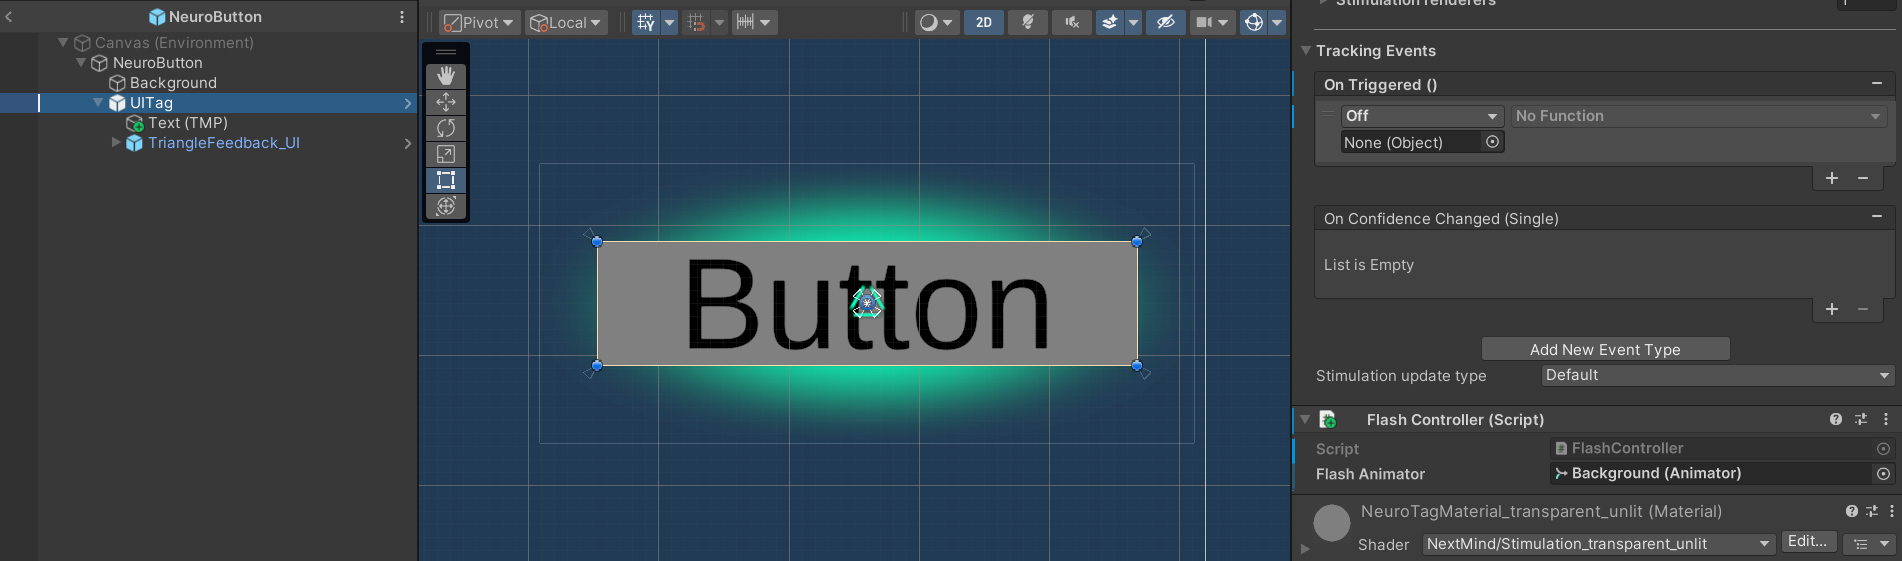
\includegraphics[width=1\linewidth]{figures/prefab-neurobutton.png}
\caption{Prefab del NeuroButton}
\label{figure:prefab-neurobutton}
\end{figure}


\subsubsection{Incorporación de NeuroButtons en la escena}

Una vez creado el prefab de los NeuroButtons, se incorporaron a la escena de Unity. Esto se logró simplemente arrastrando el prefab de cada NeuroButton dentro del canvas de la escena.



Cada NeuroButton se asoció con una dirección específica del pan-tilt: arriba, abajo, izquierda y derecha. Para lograr esto, se asignó a cada botón una función diferente que se activaría al enfocar el NeuroTag correspondiente. Es importante resaltar que, para proporcionar una interacción tanto por interfaz cerebral como por interfaz tradicional (mouse), se asignó la misma función tanto al evento de ``onTrigger'' del NeuroTag como al evento de ``onClick'' del botón. De este modo, se puede realizar la misma acción ya sea haciendo clic con el mouse o enfocando con la atención el NeuroTag.



Este tipo de configuración dual permite que el sistema sea operable tanto con el dispositivo NextMind como sin él, proporcionando así un grado de flexibilidad y adaptabilidad en función de las circunstancias del usuario o del ambiente de uso. Además, añade una capa de redundancia que puede resultar útil en caso de problemas técnicos con el dispositivo NextMind o en situaciones en las que el usuario quiera interactuar con el sistema de una manera más tradicional.



Es importante señalar que se encontró un problema común cuando se trabajaba con NeuroTags dentro de un canvas en Unity: los NeuroTags pueden fallar en esta configuración. Este problema está documentado en la página de problemas conocidos y soluciones del SDK de NextMind\cite{NextMindKnownIssues}.



Para solucionar este problema, se cambió el modo de renderizado (Render Mode) del canvas en el Inspector a ``Screen - Space: Camera''. Posteriormente, se arrastró la cámara principal (Main Camera) de la escena al campo ``Render Camera''. Este ajuste garantiza que los NeuroTags se renderizan correctamente, permitiendo su detección y activación.

\subsection{Integración de Ros2forUnity con NeuroButtons}

\subsubsection{Prefab de inicialización de ROS2}
Teniendo la instalación realizada del asset Ros2ForUnity (véase el apéndice \ref{ros2forunity}). La integración con NeuroButtons se realizó de la siguiente manera. Se crea un prefab de inicialización de ROS2 que contiene dos scripts: un ROS2 Unity Component, siguiendo la guía oficial de Ros2ForUnity\footnote{Ros2ForUnityUsage: \url{https://github.com/RobotecAI/ros2-for-unity\#usage}}, y Ros2Start, un código que tiene como objetivo crear un nodo que genera un publicador para comunicarse con el Pan-Tilt y un suscriptor para recibir los mensajes del ESP32, sirviendo como canal de comunicación de log (ver ap\'endice\ref{appendix:ros2startscript}) Como este es un script de inicialización, el publicador envía un mensaje a la cámara solicitando su IP si está conectada.



Es relevante destacar que Ros2Start implementa el patrón Singleton, asegurando que, una vez creada la instancia, no se destruye ni se recrea, garantizando un funcionamiento constante incluso durante los cambios de escena. Esta implementación es esencial para mantener la recepción de mensajes del suscriptor, que se discutirá en la sección \ref{subsection:subscriptor}. Igual que Ros2Start, el suscriptor también implementa el patrón Singleton para garantizar la continuidad y coherencia de la gestión de mensajes entrantes.



El patrón Singleton se implementa mediante el uso del método Awake(). Cuando Unity instancie la clase correspondiente, este método será el primero en ejecutarse. Si ya existe una instancia de la clase objetivo (significando que Instance no es nula), el objeto actual se destruirá para asegurar la unicidad de la instancia. En caso contrario, Instance se establecerá como el objeto actual, y gracias a DontDestroyOnLoad(gameObject), la persistencia de este objeto se garantiza a lo largo de los cambios de escena.



Es posible manejar el suscriptor directamente desde Ros2Start, sin embargo, para mantener la claridad y organización del código, se decidió separar esta funcionalidad en un archivo distinto.



Antes de describir el funcionamiento del código, es útil entender los desafíos que presenta la gestión de mensajes entrantes en aplicaciones en tiempo real, como Unity. En un entorno multihilo, múltiples procesos pueden intentar acceder y modificar los datos simultáneamente, potencialmente conduciendo a condiciones de carrera y otros problemas de concurrencia. Para manejar estos desafíos de manera segura y eficiente, se utilizó una cola segura para múltiples hilos (ConcurrentQueue). Esta estructura de datos permite encolar los mensajes a medida que llegan, para luego desencolarlos de manera segura para su procesamiento.

El código completo se encuentra en el apéndice \ref{appendix:ros2startscript}.

Cuando se recibe un mensaje en el tópico ``freertos\_header\_log'', este se encola para su posterior procesamiento.


Finalmente, en el método Update(), los mensajes se desencolan y se invoca el evento OnMessageReceived para cada uno de ellos.


Esta implementación permite manejar los mensajes de manera segura y eficiente, mitigando los problemas potenciales de concurrencia y optimizando el uso de los recursos. Además, el uso de un patrón de delegado y evento permite una estructura de código flexible y sostenible, ya que los manejadores de eventos pueden ser fácilmente añadidos o eliminados según sea necesario.

\subsubsection{Suscriptor}
\label{subsection:subscriptor}
El componente Ros2SubscriberHandler (véase código en el apéndice \ref{appendix:ros2subscriberhandler}) es el responsable de gestionar y procesar los mensajes recibidos a través del sistema ROS2 en el entorno Unity. Este componente implementa el patrón Singleton, como se ha mencionado anteriormente, lo que garantiza que sólo habrá una única instancia de esta clase durante toda la ejecución del programa.

Cuando se inicializa el Ros2SubscriberHandler, el método Start() se invoca automáticamente para establecer los estados iniciales de las propiedades CameraEnabled, CameraIP y ESP32Enabled. Por defecto, asumimos que no hay ninguna cámara activa, no hay ninguna dirección IP de cámara disponible, y el ESP32 no está habilitado.

El método OnEnable() desempeña un papel esencial en el procesamiento de los mensajes recibidos. Este método se activa cuando el objeto Ros2SubscriberHandler se habilita en la escena de Unity. Dentro de este, se obtiene una referencia al componente Ros2Start y se suscribe al evento OnMessageReceived. Esta suscripción implica que cada vez que se reciba un nuevo mensaje a través de ROS2 (lo que dispara el evento OnMessageReceived), se invocará el método ProcessReceivedMessage.


El método ProcessReceivedMessage es el corazón de la clase Ros2SubscriberHandler. Este es el lugar donde se desglosan y analizan los mensajes entrantes. Cada vez que se recibe un mensaje, el contenido del campo Frame\_id se divide en varias partes. Dependiendo de estas partes, se llevan a cabo diversas acciones, incluyendo la habilitación o deshabilitación de la cámara o del ESP32, y la actualización de la dirección IP de la cámara. El procesamiento de estos mensajes depende del formato y contenido esperado de los mismos en este sistema específico. Por ejemplo, si el mensaje indica que la estación objetivo se ha desconectado, se deshabilita la cámara y se borra la dirección IP de la misma.


\subsubsection{Publicador}
\label{subsubsection:publicador}
El publicador se gestiona en el script Ros2Publish (ver ap\'endince \ref{appendix:ros2publishscript}). En él hay diferentes funciones publicas para su posterior asignación a los NeuroButtons.

Para ello, se ha creado un GameObject que incluye el script Ros2Publish con funciones para publicar, en función de lo que se necesita enviar al suscriptor del ESP32. Este script se diseñó con funciones públicas, lo que permite su asignación a eventos onClick u onTrigger.



En el código publicador que se encuentra en el apéndice \ref{lst:Ros2PublishCode} y el código de la inicialización que se encuentra en el apéndice \ref{lst:Ros2StartCode}, se puede observar que los tipos de mensajes del publicador y del suscriptor son del tipo Header. Header es un tipo de mensaje en ROS2 que contiene metadatos sobre cuándo y cómo se generó la información. Este tipo de mensaje se seleccionó porque proporciona información de control adicional que resulta útil para la depuración.



El mensaje enviado siempre tiene el siguiente formato:

\begin{verbatim}
comando / datos
\end{verbatim}

En este formato, el comando consta de 4 caracteres y los datos tienen un tamaño variable, con un máximo de 100 caracteres definido por el ESP32. Se optó por esta estructura para mejorar la eficiencia, ya que en lugar de tener muchos condicionales if/else, existen unos pocos grupos grandes de if (que corresponden a los comandos), y dentro de esos condicionales if, hay una serie de if/else dependiendo de los datos. Esta división reduce el número de condicionales if/else, mejorando el rendimiento en el peor y en el caso medio.



Para asignar las funciones públicas al onClick y al onTrigger del NeuroButton, hay que añadir a un GameObject el script de Ros2Publish. Este GameObject necesita estar separado del GameObject de inicialización y del suscriptor, porque en el momento que un solo script tenga la opción de 'Don't Destroy', el GameObject entero no se destruye y además si cambiamos de escena, al estar ya creado el Ros2Publish, los NeuroButtons y cualquier cosa que tenga onTrigger u onClick se queda en estado de 'missing'. Por lo tanto, debe construirse al mismo tiempo que el botón o cualquier otro elemento interactivo.



Una vez que se ha añadido a un GameObject que se destruya y construya según se cambia y se vuelve a la escena objetivo, se puede arrastrar ese GameObject al onClick y al onTrigger según corresponda del NeuroButton, y seleccionar la función correspondiente al acto que queremos publicar. Por ejemplo, si estamos en el UpNeuroButton, se publicará el mensaje: % revisar

\begin{verbatim}
"ACT_/Up"
\end{verbatim}


\subsection{Integraci\'on de la cámara}

En esta parte del desarrollo se asume que la c\'amara incorporada al sistema debe funcionar como un servidor web  capaz de realizar un streamming HTTP de im\'agenes, es uno de los requisitos que tiene que tener dicho dispositivo (véase la sección \ref{section:camara}).

Por lo tanto, para integrar la visión de la cámara en Unity, es necesario comprender que la cámara no envía un vídeo continuo, sino que transmite imágenes MJPEG de manera sucesiva. Por tanto, será necesario procesar y separar estos paquetes.



Se procederá a detallar más adelante el proceso de separación y tratamiento de las imágenes. 

\subsubsection{Setup Inicial}
\label{subsubsection:initial-setup}

Se ha creado un Prefab denominado VideoCamera que incluye en su estructura un BackgroundRawImage, un VideoRawImage y un QueryText. La intención de estos elementos es disponer de una imagen de fondo para los momentos en los que no se reciban imágenes de la cámara, un espacio para mostrar las imágenes en directo de la cámara y un área de texto para mostrar el estado de las peticiones GET a la API REST, permitiendo además la visualización de posibles errores en la transmisión.

\subsubsection{Direcciones IP y Puertos}

La cámara utiliza una dirección IP y un puerto específico para el streaming de imágenes, y la misma dirección IP con un puerto distinto para realizar peticiones GET y así poder cambiar su estado en la captura de códigos QR o en el HUD, mediante variables enviadas en la query.

El puerto 81 es utilizado para la visualización del streaming, mientras que el puerto 80 se utiliza para realizar las peticiones GET. 

\subsubsection{Interacción con la Cámara Mediante API REST}
La petición GET para enviar un comando a la aplicación de la cámara se puede ver en el código \ref{lst:GetRequestCamera}.

\begin{lstlisting}[style=basicStyle,label={lst:GetRequestCamera}, caption={Petición get para la cámara}]
http://IP:80/app?app=C&value=V
\end{lstlisting}

Donde IP es la dirección IP del servidor web y C y V funcionan de acuerdo a una tabla específica.

En la tabla \ref{table:cam_commands} se pueden observar los distintos comandos (columna ``C'') y sus respectivos valores (columna ``V'') utilizados para las peticiones GET a la cámara. Estos comandos y valores proporcionan una serie de funciones que controlan el estado y la funcionalidad de la cámara, como el reinicio del estado interno de la aplicación, la devolución del estado interno, el establecimiento de dicho estado, el control del streaming, el cambio de modo de detección de QRs, el reinicio del sistema completo y la solicitud de detección de QR. Además, algunos de estos comandos permiten conmutar entre modos de operación dependiendo del valor proporcionado.

\begin{table}[!htb]
\begin{adjustbox}{width=\textwidth,center}
\begin{tabular}{|c|c|c|}
\hline
\textbf{C (comando)} & \textbf{V(valor)} & \textbf{Descripción} \\
\hline
0 & NA & Estado interno: Reinicia el estado interno de la aplicación a 0 \\
\hline
1 & NA & Estado interno: Devuelve el estado interno de la aplicación \\
\hline
2 & s & Estado interno: Establece el estado interno de la aplicación en s \\
\hline
3 & 0 & Control: detiene el streaming \\
\hline
3 & 1 & Control: Cambia el modo de detección de QRs a por petición \\
\hline
4 & NA & Reinicia el sistema completo tras una pausa \\
\hline
5 & 0 & Solicita detección de QR y, si está en modo continuo, la conmuta al modo por petición \\
\hline
\end{tabular}
\end{adjustbox}
\caption{Comandos y valores para peticiones GET a la cámara}
\label{table:cam_commands}
\end{table}

\subsubsection{Escena de Configuración}

Para gestionar todas estas peticiones GET desde Unity, se ha creado una escena adicional denominada ``Escena de Configuración'' (véase la figura \ref{figure:configuration-scene})

\begin{figure}[!htb]
\centering
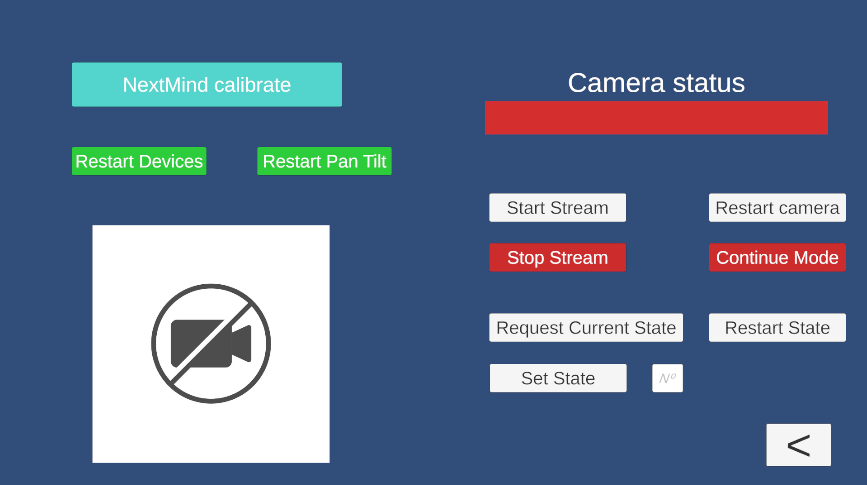
\includegraphics[width=0.8\linewidth]{figures/configuraton-scene.png}
\caption{Escena de configuración}
\label{figure:configuration-scene}
\end{figure}

La funcionalidad de los botones se establece asignando funciones públicas a sus eventos onClick, tal como se detalló anteriormente.

El resultado final en funcionamiento se puede observar en la figura \ref{figure:camera-works-configuration-scene}

\subsubsection{Procesamiento de los Mensajes Recibidos}

Siguiendo un orden lógico, primero se procesan los mensajes que llegan a través del suscriptor, mencionado previamente. En el método ProcessReceivedMessage, estos mensajes se procesan y se almacenan en atributos públicos.

\subsubsection{Clase CameraInfo}

Para mantener una organización y legibilidad óptimas, se creó el script CameraInfo (véase el código en el apéndice \ref{appendix:camerainfoscript}), que es una clase dedicada al estado de la cámara. Esta clase se encarga de recoger la dirección IP de la cámara, si está disponible, y de transformar esa IP en una URL para la captura del streaming o para preparar la URL para la API REST.

Los métodos \lstinline{GetUrl} y \lstinline{GetUrlApiRest} generan las URLs para el streaming de la cámara y para la API REST, respectivamente.

\subsubsection{Clase CameraNetworkCommandController}

Utilizando la clase CameraInfo, pudiendo obtener desde ella el GetUrlApiRest, se pueden hacer peticiones GET añadiéndole la query correspondiente. Eso es lo que trata de hacer este script, para lo que se incluyen métodos públicos con las ordenes descritas en la tabla \ref{table:cam_commands}. El código completo de la clase se puede ver en el apéndice \ref{appendix:CameraNetworkCommandController}.

\subsubsection{CameraNetworkCommandController: Método GetQR}

Como ejemplo de las funciones de la clase CameraNetworkCommandController, el método GetQR es un método público esencial que se encarga de inicializar la solicitud de detección de códigos QR.



El método GetQR es un método público esencial en esta clase, que se encarga de inicializar la solicitud de detección de códigos QR. Primero, limpia cualquier mensaje previo en el campo responseText, que se utiliza para mostrar la respuesta de la cámara. Luego, verifica el estado de la cámara a través del método GetState del objeto cameraInfo. Si la cámara no está habilitada, se interrumpe el proceso, registrando un error en el registro de Unity y en el campo responseText. Si la cámara está habilitada, se construye un comando en formato de cadena de texto (``/app?app=5\&value=0'') para solicitar la detección de un código QR. Posteriormente, se registra dicho comando en el registro de Unity para seguimiento y finalmente se inicia una corrutina llamada SendCommand que se encargará de enviar el comando a la cámara.

\subsubsection{CameraNetworkCommandController: Rutina SendCommand}

La rutina SendCommand lleva a cabo la solicitud GET de manera asíncrona, lo que significa que su ejecución se realiza en paralelo al hilo principal de Unity, permitiendo que otros procesos y animaciones sigan funcionando sin interrupciones. En esta rutina, se concatena el comando con la URL base de la API REST de la cámara, proporcionada por el método GetUrlApiRest del objeto cameraInfo, formando así la URL completa de la solicitud GET. Se configura un tiempo de espera de 60 segundos y se envía la petición. Una vez que se recibe la respuesta, se procesa y se muestra en el campo responseText, ofreciendo feedback sobre la operación realizada. En caso de producirse algún error durante la solicitud, se gestiona adecuadamente, proporcionando información detallada sobre la naturaleza del error.



Se modificó el tiempo de espera porque la conexión con la cámara es bastante lenta.

\subsubsection{CameraNetworkCommandController: Método SetState}

El método \lstinline{SetState} tiene un comportamiento un poco diferente, ya que incluye un paso adicional antes de formar y enviar el comando. En este caso, se requiere un valor de entrada proporcionado por el usuario para cambiar el estado de la cámara. Este valor se introduce a través del campo setStateInputField. Se realiza un intento de convertir el texto introducido a un número entero utilizando int.TryParse(). Si la conversión es exitosa, es decir, el usuario ha ingresado un número entero válido, se forma el comando con la estructura ``/app?app=2\&value='' + stateValue. Posteriormente, se registra este comando en el registro de Unity y se inicia la corutina SendCommand para enviar la petición a la cámara.



Si la conversión no es exitosa, lo que indica que el usuario ha introducido un valor no válido (no es un número entero), se registra este error en el registro de Unity y se muestra un mensaje de error en el campo responseText.



Por lo tanto, el método SetState extiende la funcionalidad de la clase CameraNetworkCommandController, permitiendo cambiar el estado de la cámara a través de comandos de entrada del usuario, al mismo tiempo que gestiona y proporciona retroalimentación adecuada sobre cualquier error potencial en el proceso.


\subsubsection{Inicialización del Streaming: ImageStreamUrl}
Para inicializar el stream, hay un botón en la escena de configuración como se puede ver en la Figura \ref{figure:configuration-scene}. Ese botón tiene asociado en el evento onClick la función StartStream del script ImageStreamUrl (véase el código completo en el apéndice \ref{appendix:imagestreamurl}) Este script contiene un software de código abierto diseñado para dividir imágenes MJPEG en segmentos manejables para que Unity pueda procesarlos y mostrarlos\footnote{Código abierto para manejar MJPEG en Unity: \url{https://gist.github.com/lightfromshadows/79029ca480393270009173abc7cad858}}.


El método \texttt{StartStream()} es un método público que se utiliza para comenzar a recibir un flujo de imágenes de la cámara. Lo que se ha modificado de este software de código abierto es que primero verifica si la cámara está habilitada utilizando el objeto CameraInfo, y muestra un error si no lo está. A continuación, obtiene la URL de la cámara a través de CameraInfo y comienza a recibir el flujo.



Para hacer esto, StartStream() crea una instancia de Thread para ejecutar el método ReadMJPEGStreamWorker(). Este nuevo hilo se ejecuta en paralelo con el hilo principal del juego de Unity, lo que permite que la recepción y el procesamiento del stream de la cámara se realice sin bloquear la ejecución del resto del juego.



El hilo se inicia con dos argumentos: un identificador único y la URL del stream de la cámara. El identificador único se genera utilizando un número aleatorio para evitar conflictos entre múltiples instancias de ReadMJPEGStreamWorker().

\subsubsection{Procesamiento y Segmentación de la Imagen: ImageStreamUrl}

El método ReadMJPEGStreamWorker() se ejecuta en un hilo separado y se encarga de leer el stream de la cámara. Utiliza el protocolo HTTP GET para solicitar el stream de la cámara desde la URL proporcionada.



A medida que se recibe el stream de la cámara, ReadMJPEGStreamWorker() lo divide en ``frames'' individuales. Cada frame se representa como un array de bytes, y se identifica por una secuencia de bytes específica que marca el inicio y el final de un frame.



Estos frames se añaden a un búfer hasta que se haya recibido un frame completo. Cuando se recibe un frame completo, se envía a Unity para que lo procese y lo muestre. Esto se hace asignando el frame al atributo ``nextFrame'' en el método Update(). Cuando Unity está listo para procesar el siguiente frame, toma el valor de nextFrame, lo procesa y lo muestra, y luego limpia nextFrame.



Si se produce un error al leer el stream de la cámara, ReadMJPEGStreamWorker() intentará reiniciar la conexión hasta un número máximo de intentos.



Por último, el método SendFrame(byte[] bytes) toma un array de bytes que representa un ``frame'' completo y lo convierte en una Texture2D. Si los datos de la imagen son válidos, se aplica a un RenderTexture que puede ser mostrado en Unity. Si los datos de la imagen no son válidos, se muestra un mensaje de error.



Este Texture2D es un atributo público para poder asignarselo desde el inspector.


\subsubsection{Visualización de Imágenes en Unity}

Se dispone de un Texture2D y una imagen de fondo destinada a ser utilizada en el fondo del prefab VideoCamera, ya que son componentes necesarios del mismo. Esta relación se puede observar en la figura \ref{figure:imagestreamurlui-videocameraprefab}. Al atributo BackgroundRawImage se le asigna la imagen de fondo (que debe ser de tipo Sprite) y al atributo VideoRawImage se le asigna el Texture2D, estableciéndose así como la textura del RawImage respectivo.



Para que este Texture2D contenga imágenes, es necesario pasarlas a ImageStreamUrl, que dispone de un atributo público de tipo Texture2D preparado para este propósito. Véase la figura \ref{figure:imagestreamurl}.

\begin{figure}[!htb]
   \centering
    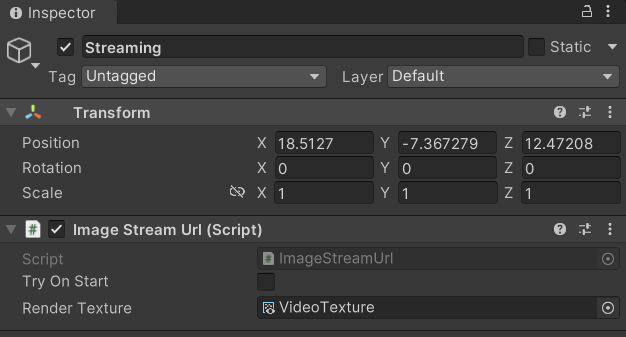
\includegraphics[width=0.75\linewidth]{figures/imagestreamurl.png}
   \caption{ImageStreamUrl en el GameObject Streaming}
   \label{figure:imagestreamurl}
\end{figure}


\subsubsection{Uso del Patrón Singleton en ImageStreamUrl}
Parece razonable que el ImageStreamUrl tenga que mantener su instancia y no poder ser borrada aunque cambiemos de escena para no perder la conexión con la cámara, así que le puse el patrón singleton para que solo existiera una sola instancia del mismo. Se le creó un GameObject único para que no afecte en la persistencia de otros GameObjects y que fuera legible y lógico semánticamente hablando. Ese GameObject se llama Streaming como se puede ver en la figura \ref{figure:imagestreamurl}. Este GameObject se encuentra en la escena principal, donde se encuentran los NeuroButtons.



Gracias a esta configuración, la Textura2D que modifica ImageStreamUrl puede ser utilizada en todas las escenas con la información completamente actualizada. La implementación de este proceso se puede observar en la figura \ref{figure:camera-works-pan-tilt-scene}.

\begin{figure}[!htb]
   \centering
    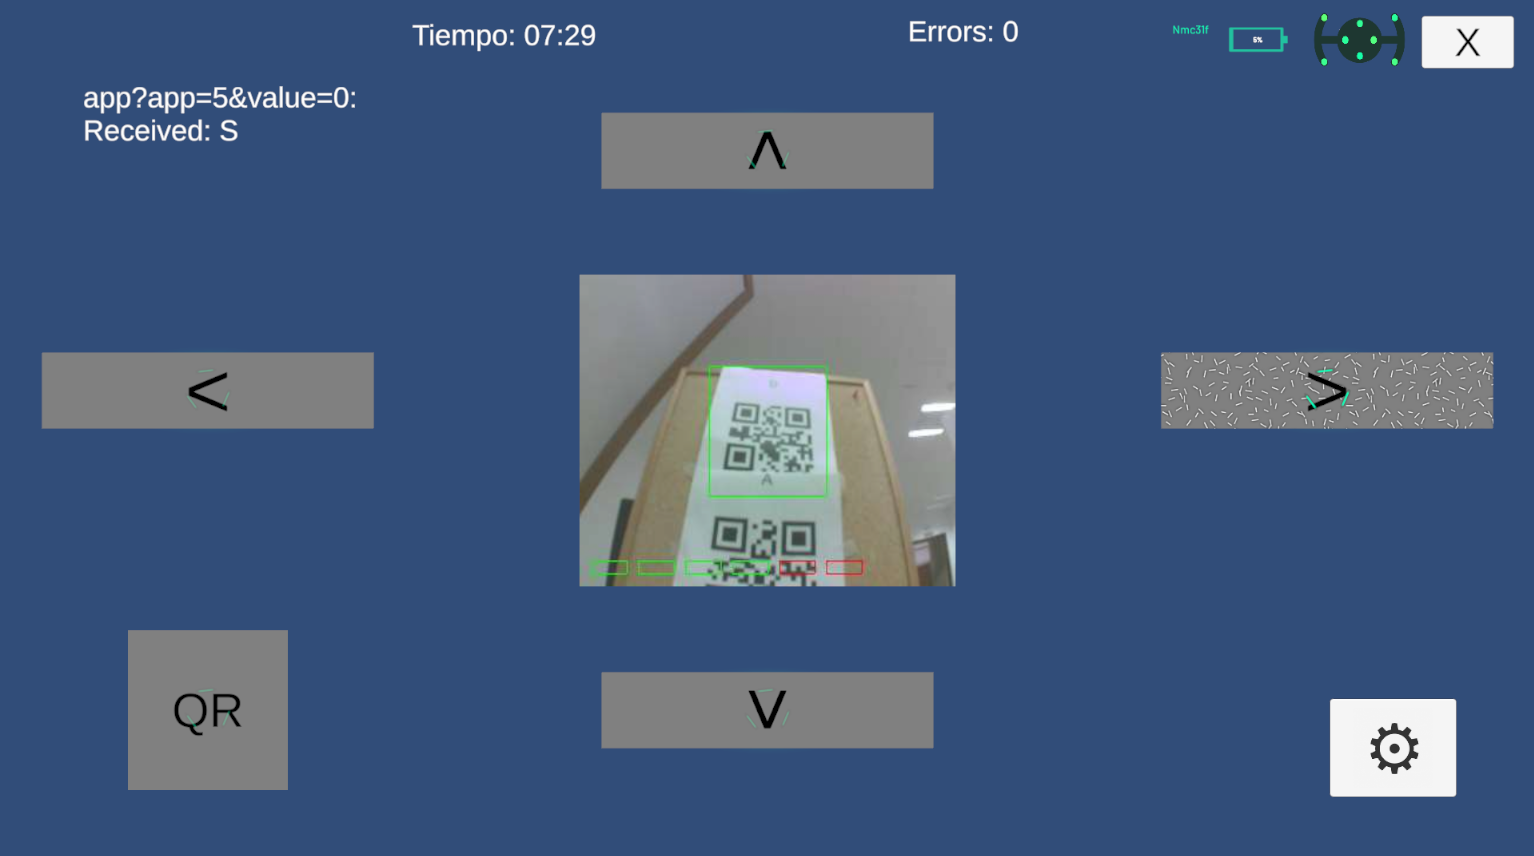
\includegraphics[width=0.8\linewidth]{figures/camera-works-pan-tilt-scene-current.png}
   \caption{Resultado final de la escena de control del Pan-Tilt}
   \label{figure:camera-works-pan-tilt-scene}
\end{figure}

\begin{figure}[!htb]
   \centering
    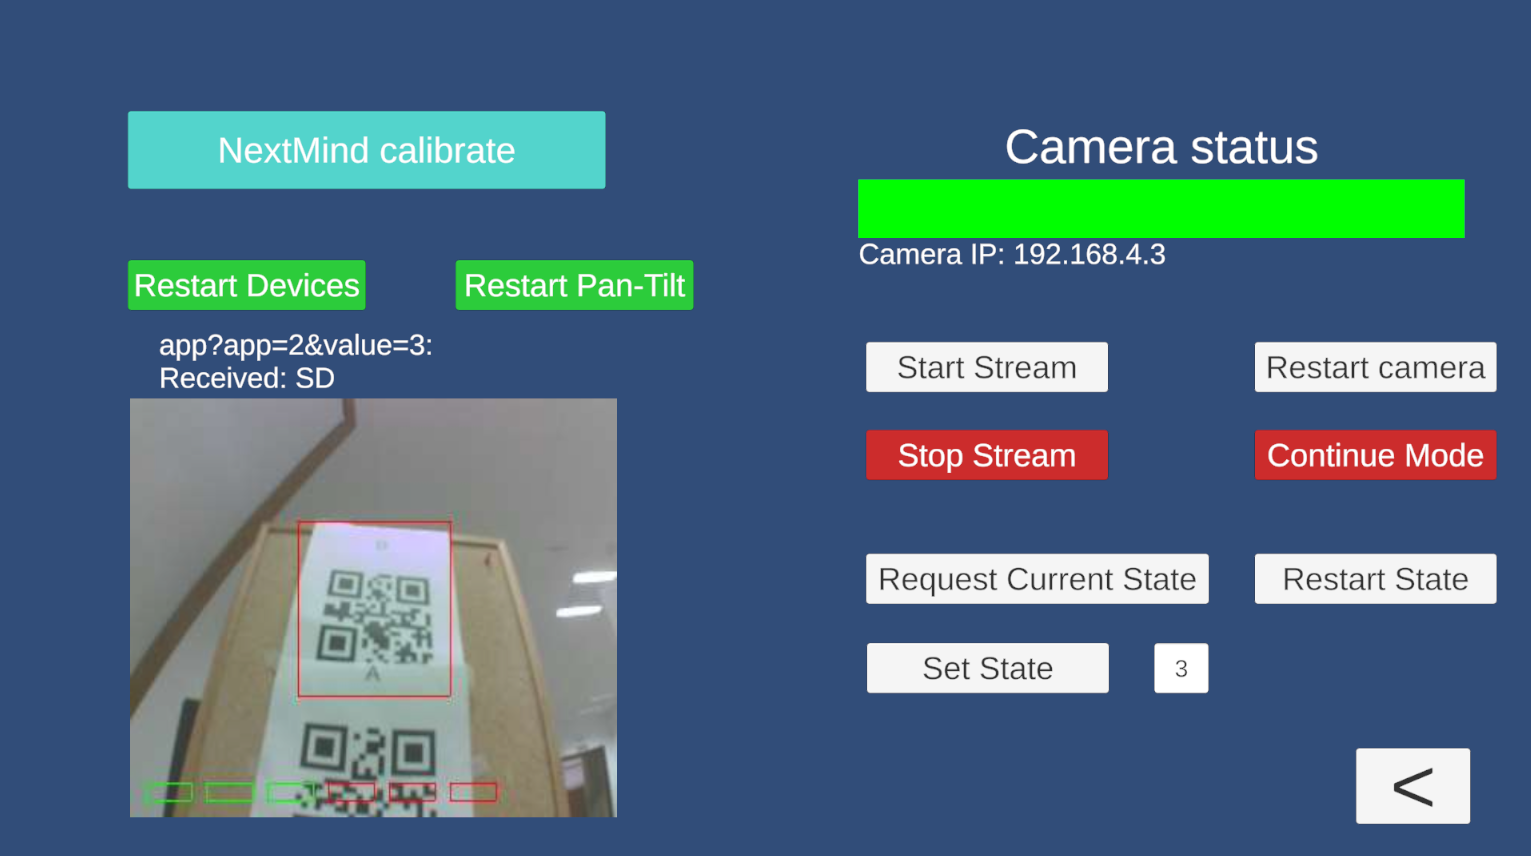
\includegraphics[width=0.8\linewidth]{figures/camera-works-configuration-scene-current.png}
   \caption{Resultado final de la escena de configuración del Pan-Tilt}
   \label{figure:camera-works-configuration-scene}
\end{figure}

\subsubsection{Asignación de CameraInfo y ErrorText: ImageStreamUrlUI}
Dado que el streaming es un objeto persistente, no se puede asignar directamente los valores de CameraInfo y ErrorText desde el inspector en función de la escena, ya que el streaming solo se encuentra en la escena principal y se perdería la referencia al objeto actual si lo asignamos de esa forma.



Para solucionar esto, se ha creado en ImageStreamUrl un método público llamado Initialize. Este método permite asignar los valores de CameraInfo y ErrorText, que son atributos privados, desde otro script que no sea persistente, es decir, que se pueda destruir y repetir en cada escena en la que se quiera mostrar el streaming. De esta forma, cada vez que nos movemos a una nueva escena, estos dos atributos se reasignan, y el objeto siempre sabe qué atributos escoger según la escena.



Se ha creado un nuevo script llamado ImageStreamUrlUI para manejar esta funcionalidad. Este script tiene como atributos públicos una instancia de CameraInfo y un ErrorText, los cuales son asignados a través del inspector. Este script ImageStreamUrlUI se añade al prefab de VideoCamera, lo que resulta en una mejoría de la comodidad de su uso.



De esta forma, el script ImageStreamUrlUI toma la instancia de ImageStreamUrl y, mediante el uso del método público Initialize, asigna los elementos CameraInfo y ErrorText en función de la escena actual (véase figura \ref{figure:imagestreamurlui-videocameraprefab})

\begin{figure}[!htb]
   \centering
    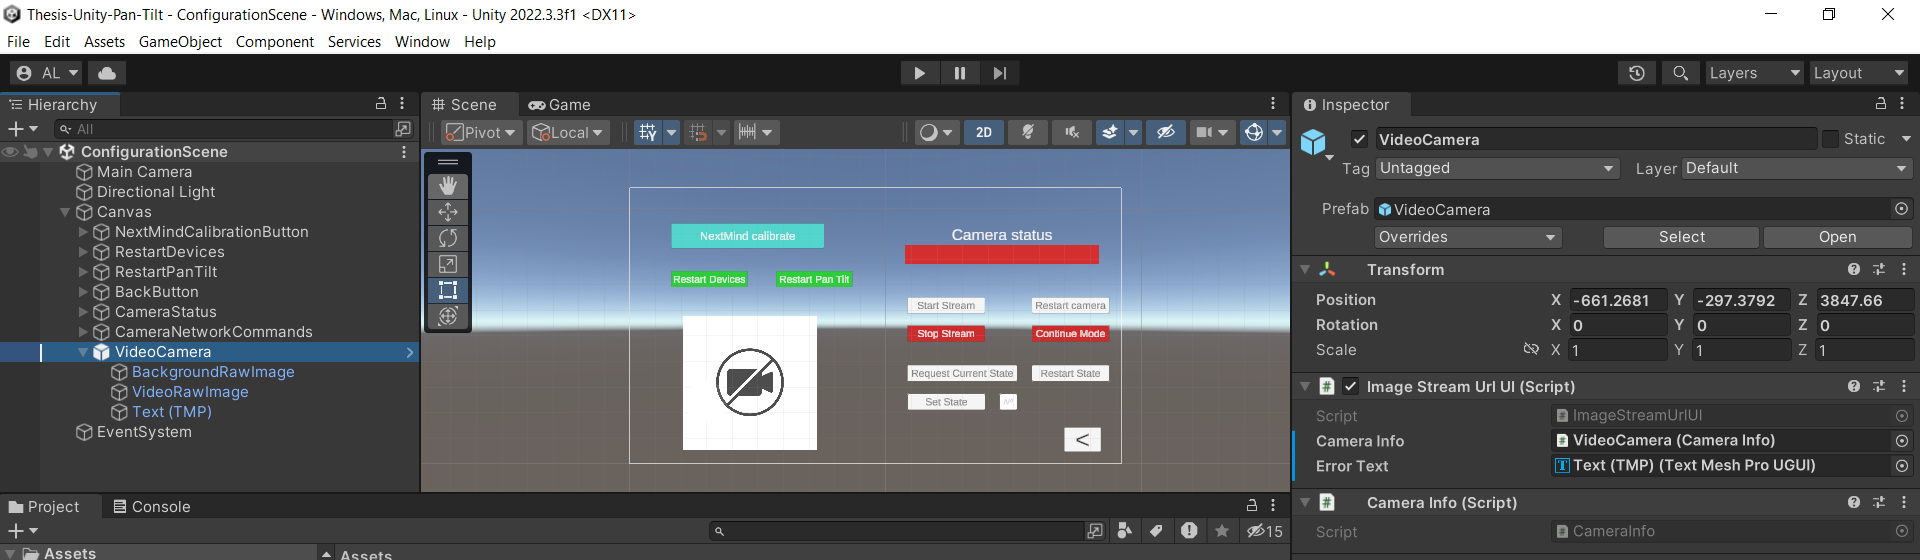
\includegraphics[width=1\linewidth]{figures/imagestreamurlui-videocameraprefab.png}
   \caption{ImageStreamUrlUI en el prefab VideoCamera}
   \label{figure:imagestreamurlui-videocameraprefab}
\end{figure}


\subsection{Botones de Control del Pan-Tilt}
En la escena de configuración quedan dos botones, uno llamado Restart Devices y otro llamado Restart Pan-Tilt.


El botón ``Restart devices'' aprovecha una peculiaridad en la gestión del WiFi, que actualmente se encuentra fuera del control de micro-ROS. Por lo tanto, no puede ser desconectado internamente, lo que da lugar a un error. Este punto será detallado más adelante en el texto. Cuando ocurre dicho error, se desencadena un reinicio total de todos los dispositivos.

Para implementar esta funcionalidad, recurrimos a un procedimiento previamente utilizado: empleamos el script ``Ros2Publish'', instanciado en un GameObject en esta escena. Luego, arrastramos ese GameObject al evento onClick correspondiente y seleccionamos la función pública apropiada.

Para obtener una comprensión más detallada de este proceso, se puede referir a la sección \ref{subsubsection:publicador}, donde se explica su funcionamiento.

Se publica el siguiente mensaje:
\begin{verbatim}
CON_/DIS
\end{verbatim}



En el Restart Pan-Tilt también es usando el mismo GameObject que tiene el Ros2Publish en esa escena. Esta vez se usa un comando 

Se publica el siguiente mensaje:
\begin{verbatim}
ACT_/Reset
\end{verbatim}










\section{Proyecto ESP-IDF: Pan-Tilt}

Además del repositorio de Unity, se maneja un repositorio aparte, ESP-IDF, que se emplea para la gestión del microcontrolador ESP32. Este repositorio se utiliza específicamente para controlar el mecanismo Pan-Tilt y la cámara, permitiendo un control eficiente y adaptativo de estos componentes.

\subsection{Configuración de Comunicación: Personalización del Transporte}

En este proyecto, la personalización del canal de comunicación se lleva a cabo mediante micro-ROS Transports, centrado especialmente en la UART (Universal Asynchronous Receiver-Transmitter) del ESP32. Este enfoque permite ajustar la comunicación a las necesidades específicas y características del hardware. Dado su papel crucial en la transmisión y recepción de datos, la UART es vital para la comunicación y control de otros dispositivos y sensores en el contexto del ESP32.



Para lograr esta personalización, se desarrolla un componente de transporte especializado. Este componente, basado en las funciones proporcionadas por micro-ROS Transports, gestiona la apertura, cierre, lectura y escritura de datos a través del puerto UART del ESP32.



El código para este componente se ha derivado de los ejemplos proporcionados en int32\_publisher\_custom\_transport\footnote{int32\_publisher\_custom\_transport: \url{https://github.com/micro-ROS/micro\_ros\_espidf\_component/tree/iron/examples/int32\_publisher\_custom\_transport}}. Sin embargo, se ha decidido convertirlo en un componente dedicado por su funcionalidad completa.



Gracias a la implementación de estas funciones, se logra establecer una comunicación personalizada utilizando la UART del ESP32 como medio de transporte. Este enfoque facilita la integración de este microcontrolador en sistemas que utilizan micro-ROS como middleware de comunicación.



El correcto despliegue de este componente requiere seguir las pautas establecidas en la sección \ref{subsection:componentcreation}.



Este componente se encarga de la inicialización del ESP32 y configura su modo de transporte.


\subsection{Gestión del Pan-Tilt: Creación de un Componente Dedicado}

Con el objetivo de controlar de manera eficaz y organizada los movimientos del sistema Pan-Tilt en el dispositivo, se desarrolló un componente específico. La estructura de este componente y la justificación de su creación se detallan en la sección \ref{subsection:componentcreation}, mientras que el código está disponible en los apéndices \ref{appendix:pantiltcontrollerheader} y \ref{appendix:pantiltcontroller}.



El componente dedicado a la gestión del Pan-Tilt se diseñó para asegurar un control preciso de la modulación de ancho de pulso (PWM), esencial para manejar correctamente los movimientos del sistema. Este aspecto del diseño del componente se explica en profundidad en la sección \ref{subsection:pwm}.



El componente se compone de varias partes, que se listan a continuación:

\begin{itemize}
    \item Constantes SERVO\_MIN\_DUTY, SERVO\_MAX\_DUTY, SERVO\_MIDDLE\_DUTY, SERVO\_MAX\_ANGLE y SERVO\_MIN\_ANGLE que definen los límites de los servomotores en términos de su ciclo de trabajo y los ángulos permitidos.
    \item Estructuras TimerState, ServoState y PanTiltState que almacenan el estado actual de los temporizadores y los servomotores.
    \item Funciones init\_horizontal\_servo, init\_vertical\_servo y init\_pwm\_timer, que inicializan los servomotores y el temporizador PWM. Incluyen además las funciones configure\_timer y configure\_servo, que configuran estos componentes utilizando la interfaz de control LEDC del ESP32.
    \item Funciones default\_pan\_tilt\_init, pan\_tilt\_init y pan\_tilt\_deinit para manejar el estado de la plataforma de pan-tilt.
    \item Funciones set\_horizontal\_angle y set\_vertical\_angle, que permiten establecer los ángulos de los servomotores horizontales y verticales, respectivamente.
    \item Funciones update\_timer\_state, 
    
    update\_horizontal\_servo\_state y update\_vertical\_servo\_state, que actualizan las estructuras de estado correspondientes.
    \item Finalmente, las funciones servo\_deinit y timer\_deinit, utilizadas para desactivar los servomotores y los temporizadores.
\end{itemize}

\subsubsection{Tests del Componente Pan-Tilt}

Para garantizar el correcto funcionamiento del componente Pan-Tilt, se han llevado a cabo una serie de pruebas. Estas pruebas ayudan a asegurar que los movimientos del sistema Pan-Tilt están bien controlados y que las funciones y estructuras que conforman el componente están trabajando según lo esperado.



El código de las pruebas se puede ver en el apéndice \ref{appendix:pantilttests}.



Las pruebas realizadas son las siguientes:

\begin{itemize}

\item{Prueba de límites máximos y mínimos de duty cycle: 
\
(TEST\_CASE(``Test max duty and min duty'', ``[pan\_tilt\_controller]'')) 
Esta prueba verifica que los límites de duty cycle de los servomotores se establecen correctamente.
}
\item{ Prueba de inicialización del Pan-Tilt \

(TEST\_CASE(``Test pan-tilt initializated'', ``[pan\_tilt\_controller]'')): \

esta prueba confirma que el sistema Pan-Tilt se inicializa correctamente.
}
\item{ Pruebas de ángulo horizontal y vertical \

(TEST\_CASE(``Test initial horizontal angle'', ``[pan\_tilt\_controller]'') \

y TEST\_CASE(``Test initial vertical angle'', ``[pan\_tilt\_controller]'')): \
estas pruebas verifican que los ángulos horizontales y verticales de los servomotores se establecen y se actualizan correctamente.
}
\item{ Prueba de incremento de movimiento \
(TEST\_CASE(``Test increment movement'', ``[pan\_tilt\_controller]'')): \
esta prueba verifica que el sistema Pan-Tilt puede cambiar su ángulo vertical con precisión, lo cual es importante para garantizar un movimiento suave y controlado.
}
\end{itemize}


Las pruebas se realizan utilizando la biblioteca Unity, que proporciona un marco para la creación de pruebas unitarias en C. Todas las pruebas pasaron con éxito, lo que indica que el componente Pan-Tilt está funcionando correctamente y puede controlar los movimientos del sistema con precisión.

\subsection{Gestión micro-ROS}
Para la gestión de micro-ROS dentro del ESP32 se ha creado una tarea específica (micro\_ros\_task).



La razón para dedicar una tarea a la gestión de micro-ROS es que este middleware necesita tiempo de procesador para gestionar las comunicaciones entre los diferentes nodos. Al dedicar una tarea a esta función, se garantiza que micro-ROS tiene el tiempo necesario para gestionar estas comunicaciones sin interferir con otras tareas que el microcontrolador pueda estar realizando.

\subsubsection{Suscriptor}
La función de callback del suscriptor es subscription\_callback. Esta función es bastante grande porque tiene que manejar una variedad de mensajes diferentes que podrían ser enviados al nodo del suscriptor.



La función de callback comienza por extraer los datos del mensaje recibido. Si el mensaje es demasiado largo, se imprime un error y la función se detiene.



A continuación, la función de callback extrae el comando y los datos del mensaje y los publica en otro tema.



Finalmente, la función de callback ejecuta diferentes acciones dependiendo del comando y los datos recibidos. Estas acciones pueden incluir inicializar la conexión WiFi como punto de acceso, desconectar la conexión WiFi, establecer los ángulos de los servos y más.

\subsubsection{Publicador}
En este proyecto, el publicador se inicializa en la función micro\_ros\_task, mediante el uso de la función rclc\_publisher\_init\_default. El publicador se configura para enviar mensajes del tipo std\_msgs\_\_msg\_\_Header al tema ``/freertos\_header\_log''.



Posteriormente, el publicador se emplea en distintas secciones del código para la transmisión de diversos mensajes. Específicamente, se utiliza en la función de devolución de llamada del suscriptor para enviar comandos y datos recibidos como registros.



Además, el publicador juega un papel importante en la gestión de conexiones WiFi. Por ejemplo, la función wifi\_event\_handler\_sap maneja diferentes eventos que pueden suceder en la red Soft Access Point (SAP). En el evento de que una estación se conecte y su MAC coincida con la MAC objetivo (la MAC de la cámara) el publicador envía un mensaje con la dirección IP de la estación recién conectada.



En caso de desconexión de una estación, el publicador informa si la estación desconectada es la estación objetivo. Si se asigna una IP a una estación, el publicador notifica la dirección IP asignada, especificando si se ha asignado a la estación objetivo.



Finalmente, durante el proceso de inicialización de la red SAP, la función wifi\_init\_softap utiliza el publicador para informar de los diversos estados del proceso, incluyendo el inicio, cualquier error durante la inicialización y la finalización del proceso.

\subsection{Manejo de la Conexión WiFi}

El ESP32 se configura como un Soft Access Point (SAP) (consulte la sección \ref{section:generalenvironment}), creando una red WiFi a la que se pueden conectar otros dispositivos. La finalidad de esta red es facilitar la comunicación entre la cámara y los demás nodos del sistema. El ESP32 publica información sobre los eventos de la red a través de un tema en micro-ROS, como la conexión y desconexión de estaciones, así como la asignación de direcciones IP a las mismas.



El manejador de eventos WiFi, la función \texttt{wifi\_event\_handler\_sap}, se invoca cuando ocurren eventos específicos en la conexión WiFi. Dependiendo del tipo de evento, la función realiza acciones distintas:

\begin{itemize}
    \item Cuando una estación se conecta al SAP, se desencadena el evento
    
    \texttt{WIFI\_EVENT\_AP\_STACONNECTED}. Aquí, se obtiene y publica la dirección MAC de la estación conectada.
    \item El evento \texttt{WIFI\_EVENT\_AP\_STADISCONNECTED} se activa cuando una estación se desconecta del SAP. En este escenario, se publica un mensaje informando de la desconexión. Si la estación desconectada corresponde a la \texttt{target\_mac}, se envía un mensaje adicional notificando que la estación objetivo se ha desconectado, y se marca la variable \texttt{sap\_ip\_target\_assigned} como false.
    \item Al asignarse una dirección IP a una estación conectada al SAP, se genera el evento \texttt{IP\_EVENT\_AP\_STAIPASSIGNED}. Si la estación a la que se le ha asignado la IP coincide con la \texttt{target\_mac}, se guarda la IP asignada en la variable \texttt{sap\_ip\_target} y se configura \texttt{sap\_ip\_target\_assigned} como true. Luego, se publica un mensaje notificando que la estación objetivo ha obtenido una dirección IP.
\end{itemize}

Las funciones \texttt{get\_camera\_ip} y \texttt{get\_target\_ip} se utilizan para recuperar la dirección IP de la estación objetivo y verificar si a dicha estación se le ha asignado una IP, respectivamente.



Finalmente, la función \texttt{wifi\_init\_softap} se encarga de la inicialización del SAP. Configura el SAP con los parámetros establecidos en la estructura \texttt{wifi\_config\_t}, registra el controlador de eventos \texttt{wifi\_event\_handler\_sap} para los eventos WiFi y el evento \texttt{IP\_EVENT\_AP\_STAIPASSIGNED}. Tras la configuración del SAP, se inicia el WiFi y se envía un mensaje que indica la finalización de la inicialización del SAP.



\subsubsection{Control de la Cámara a través de WiFi}

El sistema de control de la cámara debe estar diseñado para establecer una conexión automática a la red WiFi generada por el ESP32. La cámara tiene preconfigurada lacredenciales de la red WiFi del ESP32, lo que permite que se conecte de manera automática en cuanto se detecta la presencia de la red WiFi. Este enfoque asegura una conexión estable y confiable entre la cámara y el ESP32, facilitando el control y la comunicación sin necesidad de configuraciones adicionales.


\section{Puesta en marcha del sistema}

En esta sección se describirán las acciones necesarias para poner en marcha el sistema en un entorno Windows, haciendo uso del subsistema Windows para ejecutar un agente Microros conectado al dispositivo por medio de una conexión USB-Serial.


\subsection{Actuaciones en Powershell de Windows}

Para poner en marcha el proyecto primero hay que montar el setup de ROS2 en Powershell de la siguiente forma:

\begin{verbatim}
C:\dev\ros2\_humble\local\_setup.ps1
\end{verbatim}

Y abrir el proyecto de Unity en la misma Powershell

\begin{verbatim}
unity.exe -projectPath "D:\Unity\Unity Projects\Thesis-Unity-Pan-Tilt\"
\end{verbatim}

Luego usar el programa usbipd para atar los puertos correspondientes a WSL2 (véase sección \ref{WLS-considerations})
En este paso hay que asegurarse de que ya estamos conectados al WiFi del ESP32 (véase la figura \ref{figure:usbipd-in-the-lan})

\begin{figure}[!htb]
   \centering
    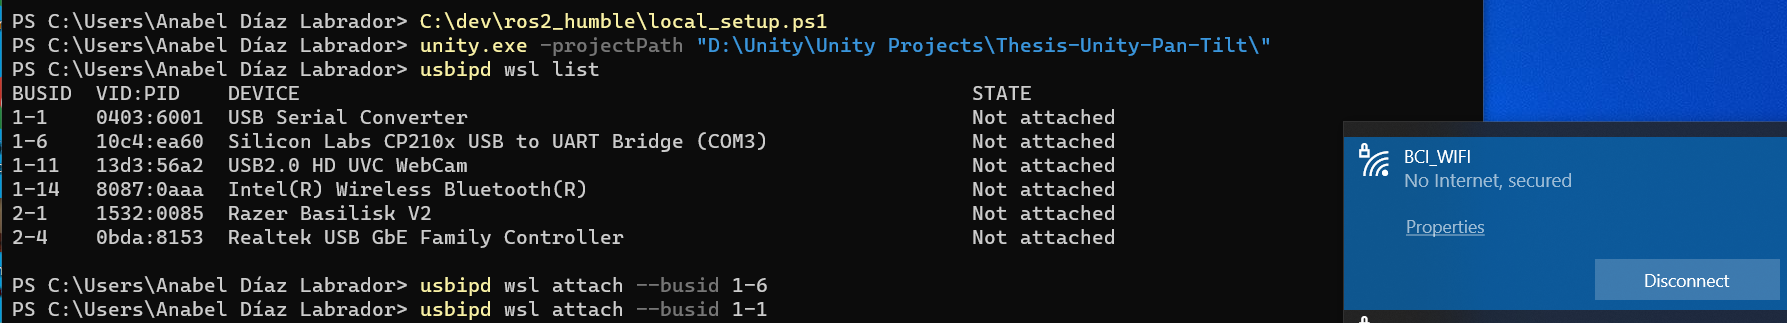
\includegraphics[width=0.8\linewidth]{figures/usbipd-in-the-lan.png}
   \caption{Preparación del proyecto en Windows}
   \label{figure:usbipd-in-the-lan}
\end{figure}

El comando para atar el puerto a WSL2 con usbipd es:

\begin{verbatim}
usbipd wsl attach --busid BUSID
\end{verbatim}

Donde BUSID es el busid correspondiente.

\subsection{Actuaciones en Ubuntu sobre WSL2}

\subsubsection{Agente de micro-ROS}

En una terminal de WSL2 hay que dar permisos a los puertos, por ejemplo si hemos atado el microcontrolador y la cámara (esta \'ultima solo en caso de que sea necesario su monitorizaci\'on) sería así:

\begin{verbatim}
sudo chmod 777 /dev/ttyUSB0
sudo chmod 777 /dev/ttyUSB1
\end{verbatim}

Se realiza ahora un source install/setup.bash del repositorio del agente de microros (véase el apéndice \ref{section:microrosagent}), para hacer que esta aplicaci\'on est\'e disponible para ROS2.

Finalmente, ejecutamos el agente de micro-ROS poniendo el puerto correspondiente:

\begin{verbatim}
ros2 run micro_ros_agent micro_ros_agent serial --dev /dev/ttyUSB0
\end{verbatim}


\subsubsection{Monitorizaci\'on de la cámara}

En otra terminal de WSL2 se necesita establecer como entorno de desarrollo ``esp-idf v4'' haciendo un source al script de exportaci\'on de esta versi\'onde la toolchain (v\'ease  \ref{section:cameraenvironmentinstallation}) 

\begin{verbatim}
get_idf4
\end{verbatim}

Primer es necesario compilar el firmware e introducirlo en el microcontrolador

\begin{verbatim}
idf.py build
idf.py -p /dev/ttyUSB1 flash
\end{verbatim}

Luego se puede monitorear de la siguiente manera:

\begin{verbatim}
idf.py -p /dev/ttyUSB1 monitor
\end{verbatim}


\section{Funcionamiento del prototipo}
\label{section:prototype-working}
El sistema presenta una interfaz intuitiva y directa. Su funcionamiento sigue un esquema de ``apunta y dispara'', donde el usuario debe centrar el código QR en un cuadrado designado como punto de mira en la interfaz de la cámara. Seis rectángulos ubicados en la parte inferior del HUD de la cámara se iluminan en verde al detectar códigos QR.



Incorpora cuatro NeuroButtons (véase sección \ref{subsubsection:add-neurotag}) que controlan el movimiento del sistema Pan-Tilt en cuatro direcciones: arriba, abajo, izquierda y derecha. El HUD de la cámara, ubicado centralmente, alberga un cuadrado que permanece constantemente en rojo, cambiando a verde cuando se detecta exitosamente un código QR. Se puede ver prototipo entero conectado y montado en la figura \ref{figure:prototipo-working}.

\begin{figure}[!htb]
   \centering
    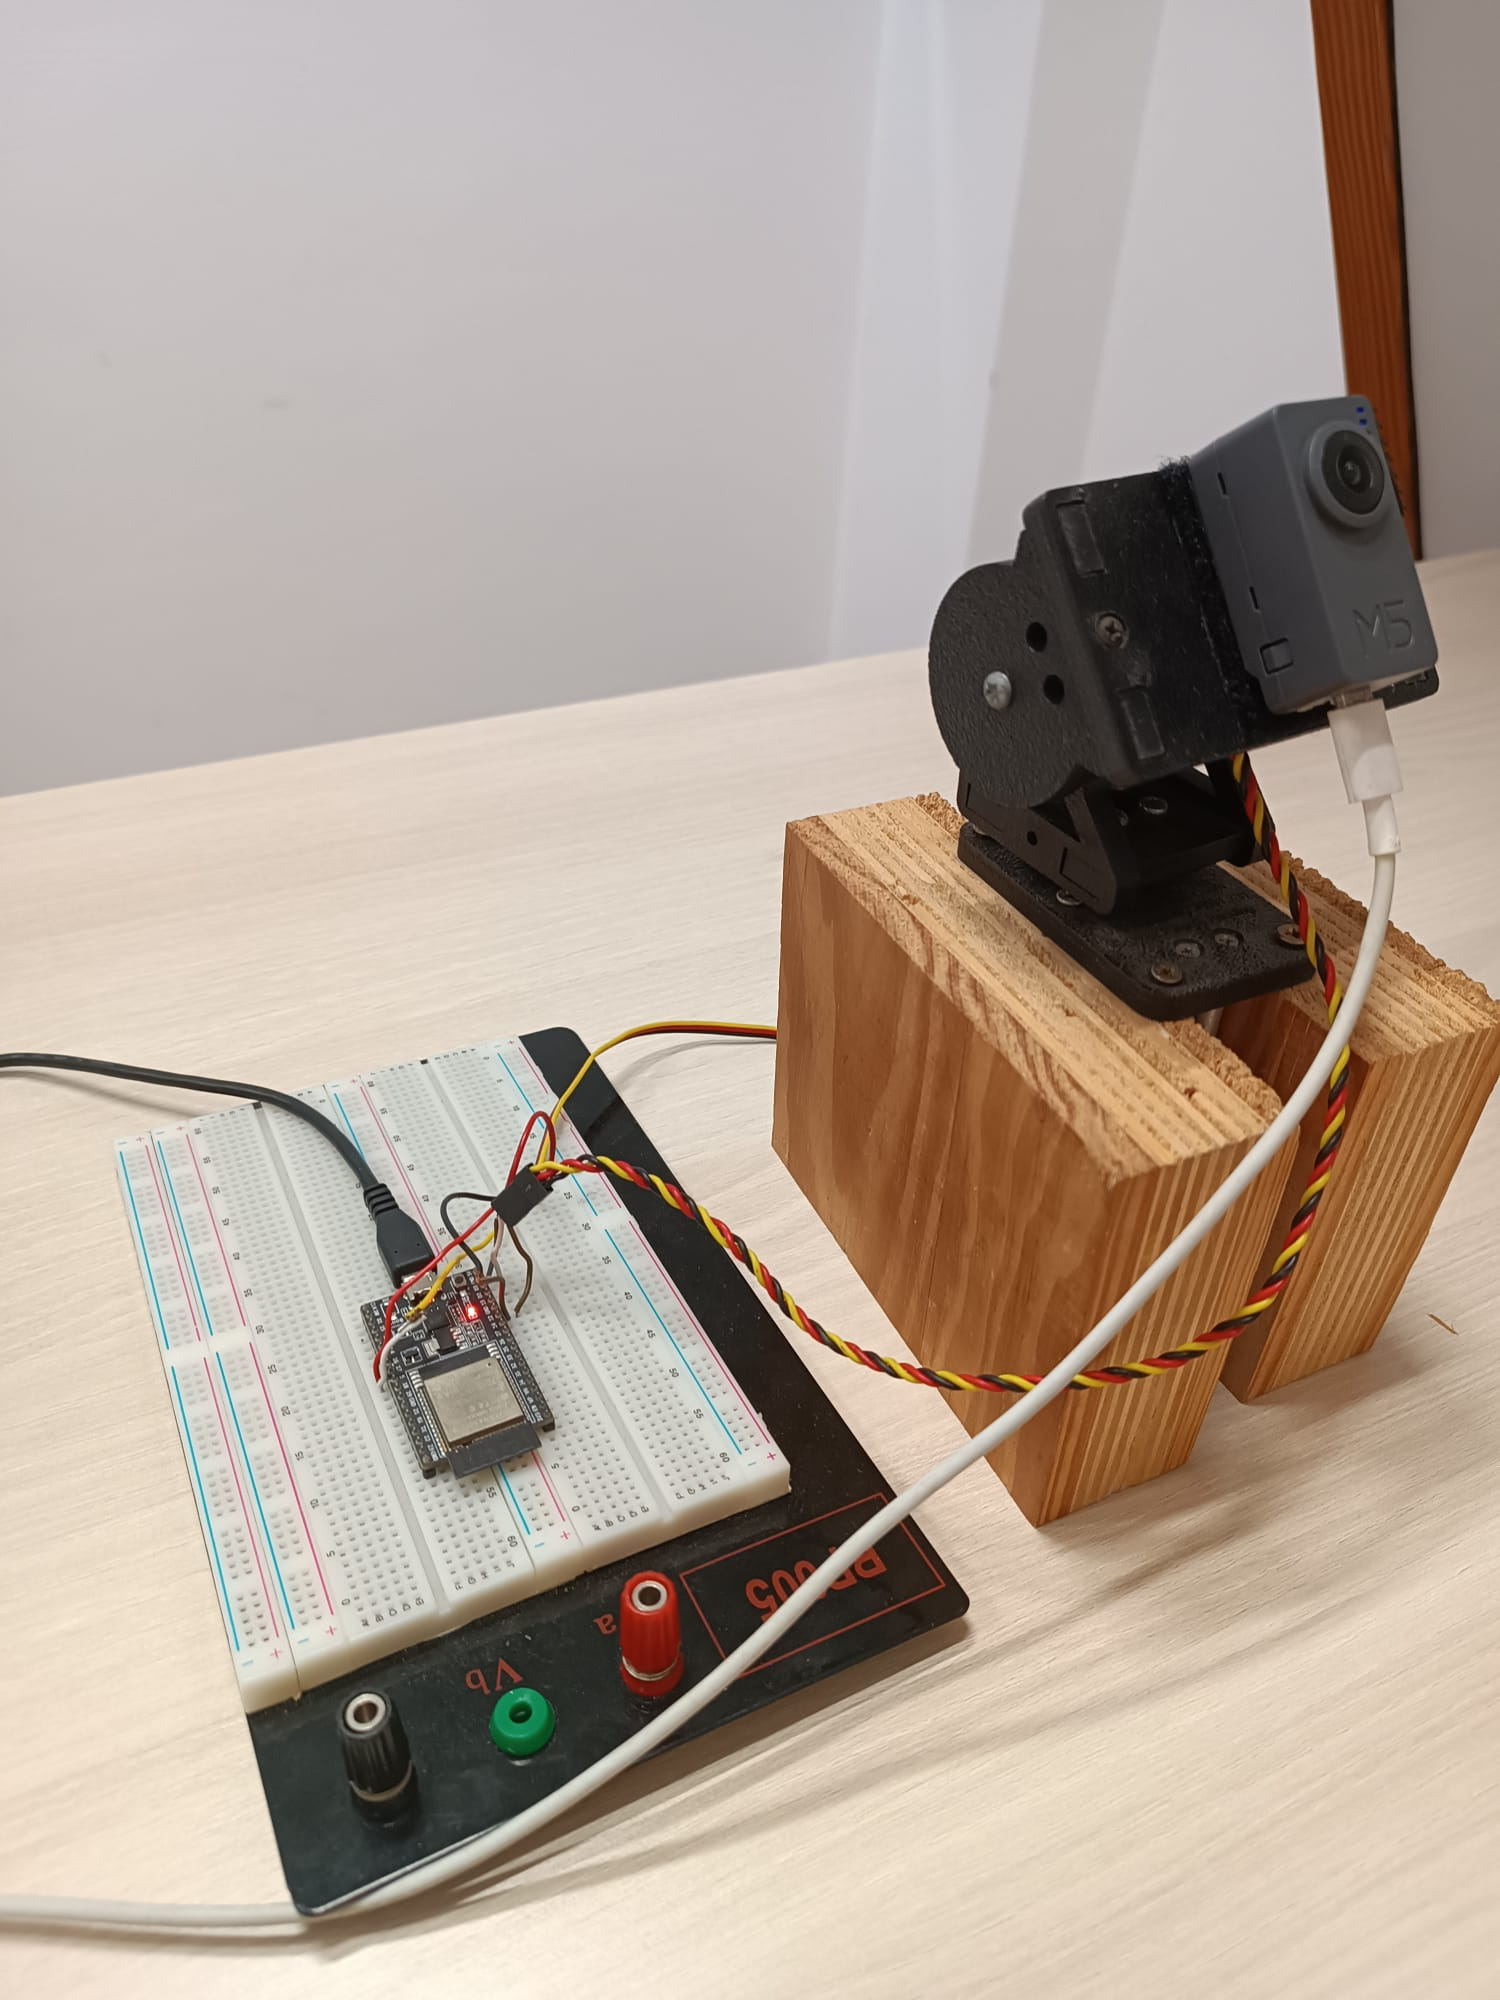
\includegraphics[width=0.35\linewidth]{figures/prototipo.jpg}
   \caption{Prototipo montado y conectado}
   \label{figure:prototipo-working}
\end{figure}

%%%%%%%%%%%%%%%%%%%%%%%%%%%%%%%%%%%%%%%%%%%%%%%%%%%%%%%%%
\newpage{\pagestyle{empty}}
\thispagestyle{empty}

\chapter{\LARGE Analisis de la experimentación y resultados obtenidos}
\label{chapter:analysisTestAndResults}

En este capítulo se abordará la evaluación del sistema desde dos perspectivas distintas.



En primer lugar, se realizará una evaluación del sistema Pan-Tilt, centrando nuestra atención en la experiencia del usuario. Se analizarán diferentes aspectos, como la facilidad de uso, la interacción y la respuesta del sistema a los comandos del usuario.



En segundo lugar, se enfoca en la flexibilidad de la interfaz, evaluando su capacidad para adaptarse a otro sistema. Específicamente, se estudiará su adaptación a un robot móvil, que incorporará un nodo de micro-ROS inalámbrico. Este nodo operará a través del protocolo UDP.

\section{Detalles de las pruebas realizadas}

Siguiendo la metodología empírica descrita en la sección \ref{researchmethodology}, este capítulo est\'a dedicado a proporcionar un panorama más detallado de las pruebas realizadas con los participantes. Las pruebas se llevaron a cabo en la Escuela Superior de Ingeniería y Tecnología (ESIT) de la Universidad de La Laguna, donde 16 participantes experimentaron con la aplicación de control Pan-Tilt en diversas condiciones de iluminación. Tras un periodo de calibración del BCI, los participantes afrontaron una prueba de diez minutos para recorrer un circuito de códigos QR (véase figura \ref{figure:entorno-prueba}). Se recopilaron datos sobre fallas del BCI, tiempos de calibración y de recorrido, los cuales han resultado esenciales para el análisis en profundidad presentado en las siguientes secciones.



Hay que tener en cuenta que la muestra recogida es bastante pequeña. 



La prueba implica la navegación a través de un circuito diseñado con códigos QR, utilizando un sistema Pan-Tilt equipado con una cámara. Los participantes debían completar el recorrido en un tiempo no superior a 10 minutos. La prueba se ejecuta dentro de una aplicación Unity, la cual incorpora una serie de NeuroTags para la manipulación del movimiento del sistema Pan-Tilt. El funcionamiento del prototipo se detalla en la sección \ref{section:prototype-working} y se visualiza en la figura \ref{figure:camera-works-pan-tilt-scene}.


\begin{figure}[!htb]
   \centering
    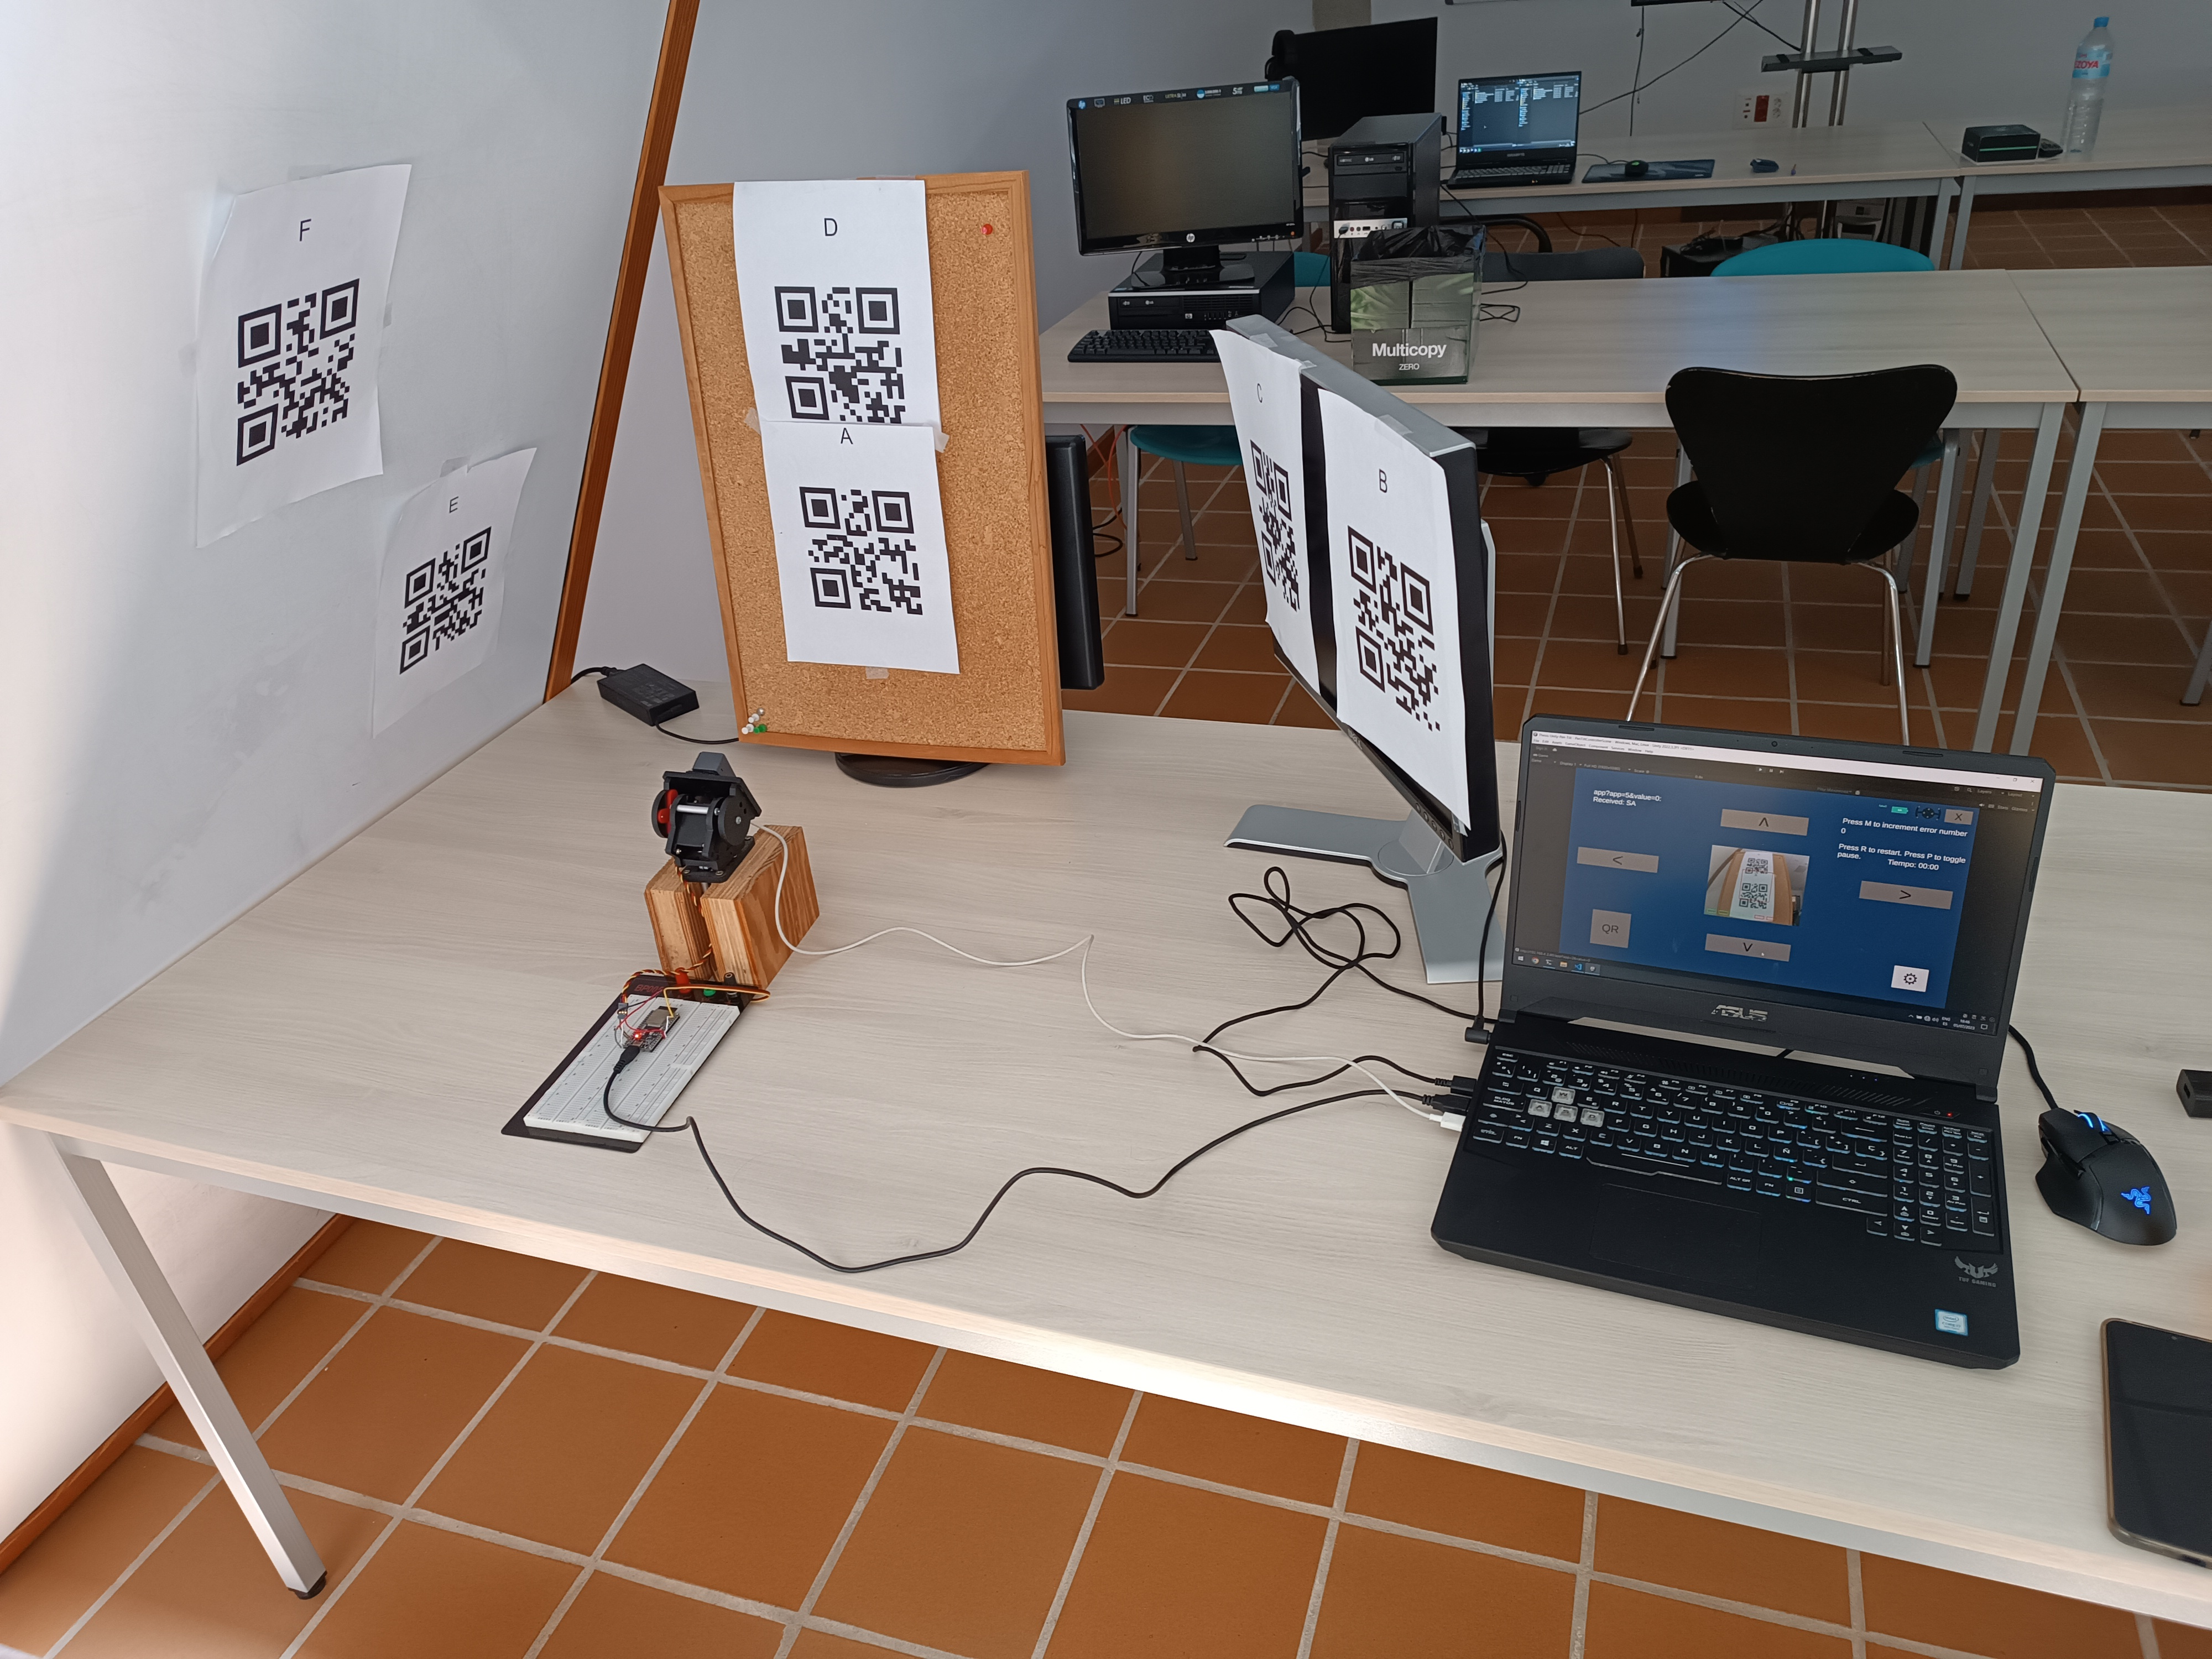
\includegraphics[width=0.7\linewidth]{figures/entorno-prueba.jpg}
   \caption{Circuito de QR}
   \label{figure:entorno-prueba}
\end{figure}

\begin{figure}[!htb]
   \centering
    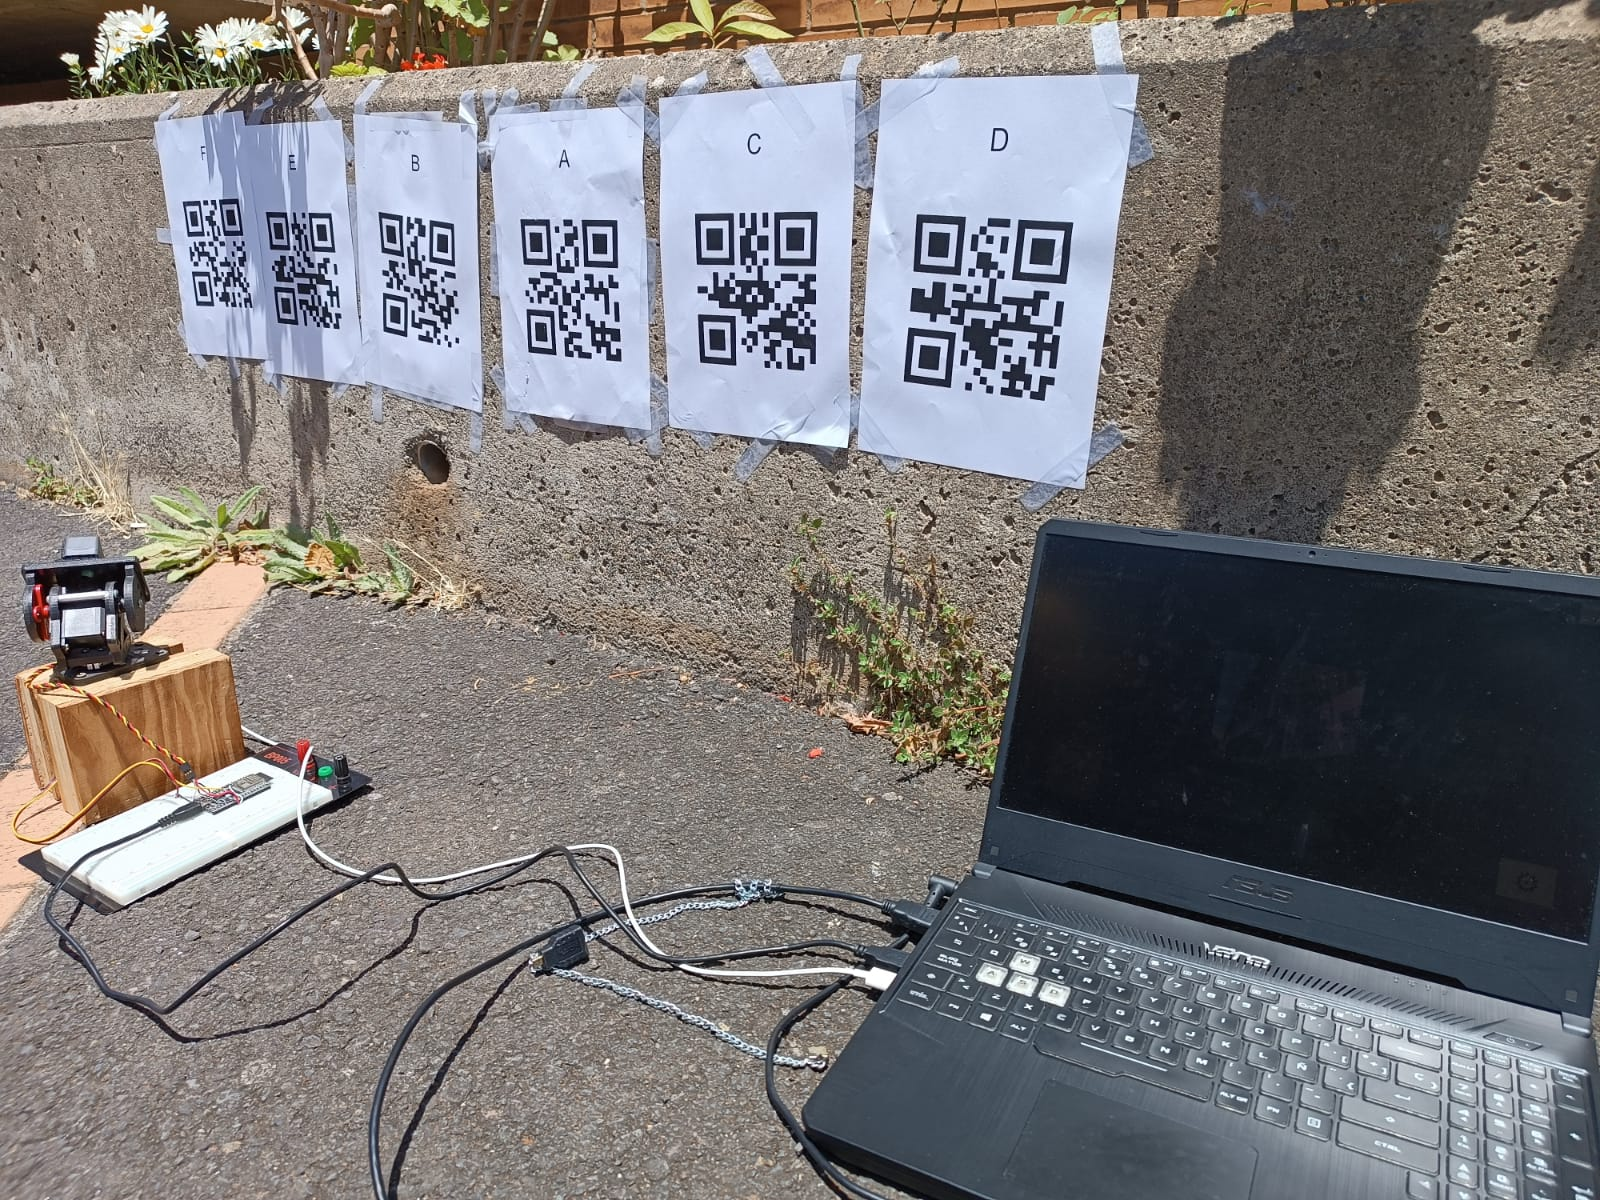
\includegraphics[width=0.7\linewidth]{figures/entorno-prueba-exterior.jpg}
   \caption{Circuito de QR en el exterior}
   \label{figure:entorno-prueba-exterior}
\end{figure}


\begin{figure}[!htb]
   \centering
    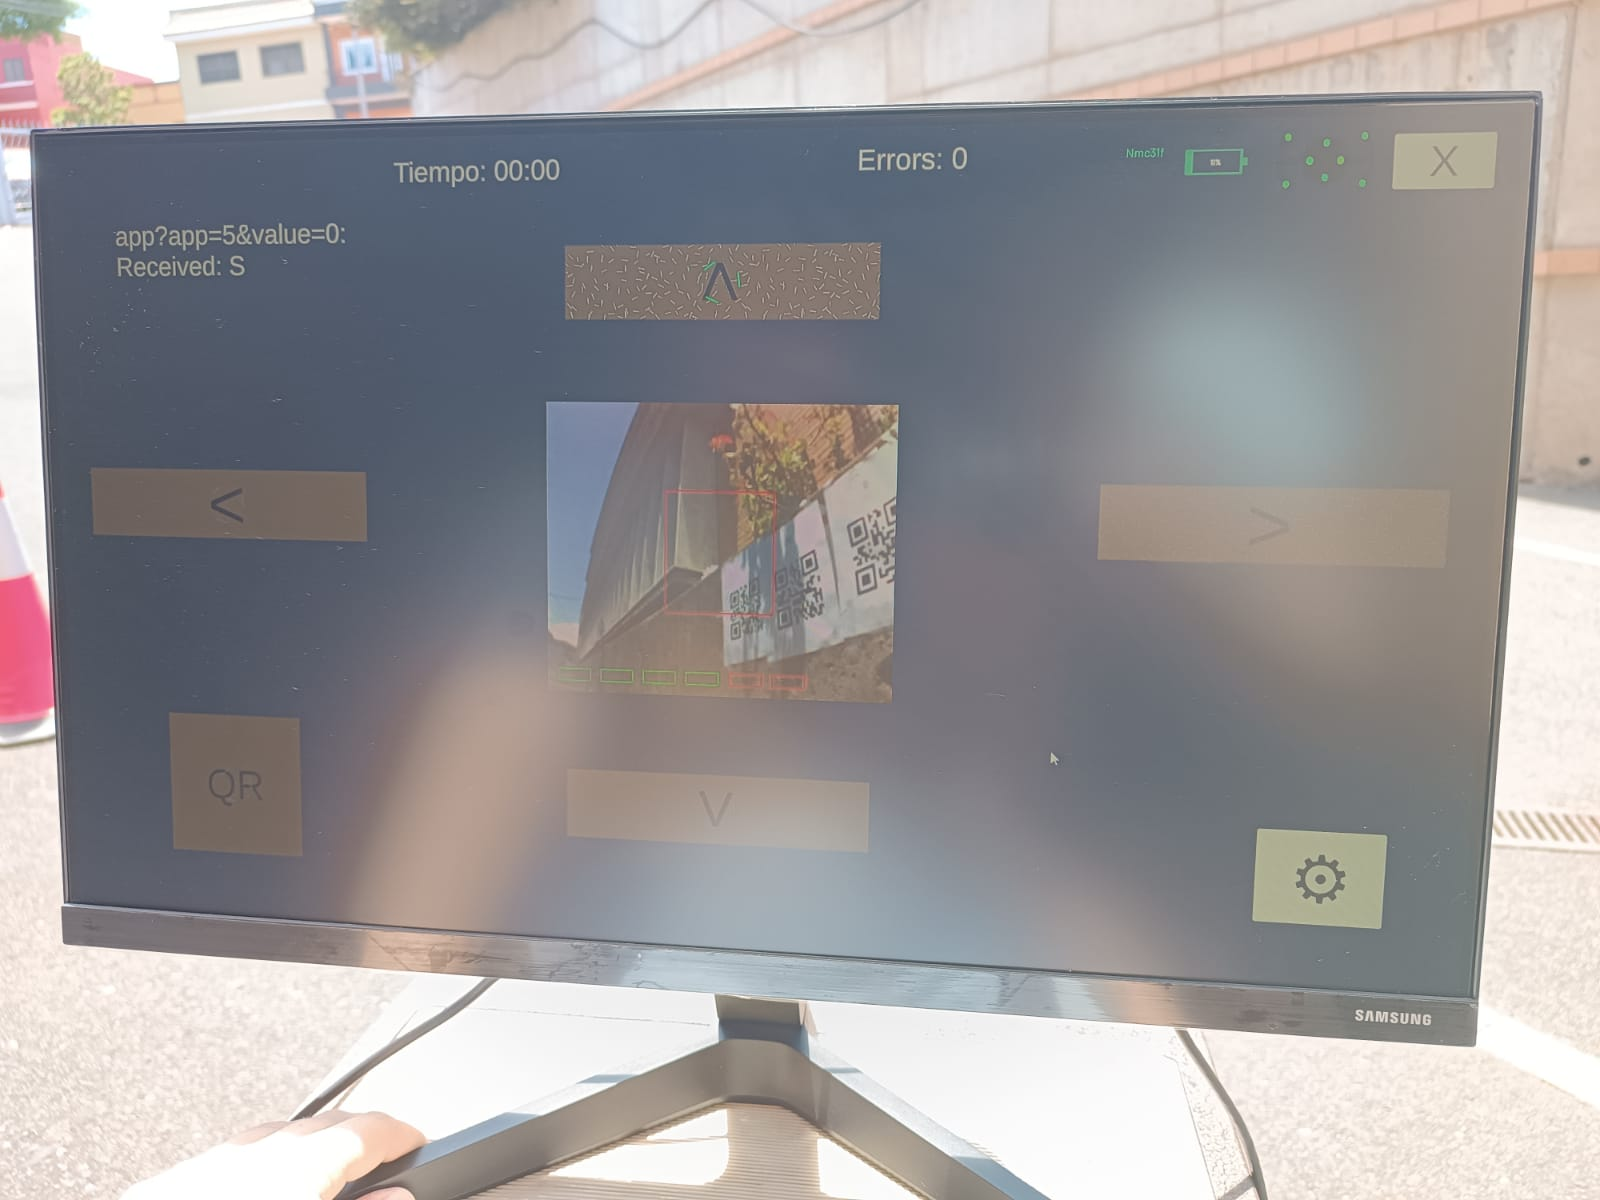
\includegraphics[width=0.6\linewidth]{figures/aplicacion-exterior.jpg}
   \caption{Prototipo Unity en el exterior}
   \label{figure:aplicacion-exterior}
\end{figure}



\section{Presentación de los datos obtenidos}
Los datos obtenidos de los 16 participantes se presentan en la tabla \ref{tab:relevantData}. Esta incluye variables como el tipo y la longitud del pelo, la nota de calibración, la luminosidad durante el uso del dispositivo y el tiempo total de uso de la interfaz cerebro-computadora (BCI).



La longitud y el tipo de pelo se recogieron debido a su potencial impacto en la capacidad del dispositivo NextMind de leer correctamente las señales cerebrales. Este aspecto es esencial para comprender las limitaciones de la interfaz en poblaciones con diferentes tipos de cabello y longitud.



Se ha dado especial importancia a la luminosidad, considerando que el estudio está orientado hacia el uso del dispositivo en exteriores. La luz ambiental podría afectar la precisión de la interfaz, posiblemente debido a los reflejos en la superficie del dispositivo o la alteración de las señales que este intenta leer.



La nota de calibración, que es una medida de cuán precisamente se ajustó el dispositivo a las necesidades individuales del usuario, se ha correlacionado con el número de errores cometidos durante el uso y el tiempo total de uso del BCI (Tiempo BCI). Esta relación es clave para evaluar el impacto de una calibración adecuada en el rendimiento del dispositivo.



El tiempo total de uso del BCI (Tiempo BCI) y el número de errores que el usuario cometió mientras utilizaba la interfaz se registraron para determinar la efectividad y la facilidad de uso del dispositivo.



Por último, se consideró si los usuarios pudieron completar las pruebas asignadas en el tiempo establecido. Si no se podía realizar la prueba, se les asignaba el tiempo máximo posible de 10 minutos, proporcionando una medida de la duración máxima de la prueba en las circunstancias más desfavorables.


\begin{table}[!htb]
\centering
\resizebox{1\textwidth}{!} {
\begin{tabular}{|c|c|c|c|c|c|c|}
\hline
\begin{tabular}[c]{@{}c@{}}Longitud\\ del\\ pelo\end{tabular} & \begin{tabular}[c]{@{}c@{}}Tipo\\ de\\ pelo\end{tabular} & \begin{tabular}[c]{@{}c@{}}Nota\\ de\\ Calibración\end{tabular} & Luminosidad & \begin{tabular}[c]{@{}c@{}}Tiempo\\ BCI\end{tabular} & \begin{tabular}[c]{@{}c@{}}Número\\ de\\ errores\end{tabular} & \begin{tabular}[c]{@{}c@{}}¿Pudo realizar la prueba?\end{tabular} \\ \hline
Mediano/Corto                                                 & Rizado                                                   & 2                                                               & Baja        & 05:50                                                & 4                                                             & Sí                                                           \\ \hline
Rapado/Calvo                                                  & Lacio                                                    & 4                                                               & Media       & 06:32                                                & 5                                                             & Sí                                                           \\ \hline
Mediano/Corto                                                 & Rizado                                                   & 3                                                               & Media       & 05:05                                                & 4                                                             & Sí                                                           \\ \hline
Rapado/Calvo                                                  & Lacio                                                    & 1                                                               & Baja        & 10:00                                                & -                                                             & No                                                           \\ \hline
Largo                                                         & Rizado                                                   & 1                                                               & Baja        & 10:00                                                & -                                                             & No                                                           \\ \hline
Rapado/Calvo                                                  & Lacio                                                    & 5                                                               & Baja        & 03:51                                                & 0                                                             & Sí                                                           \\ \hline
Largo                                                         & Lacio                                                    & 3                                                               & Baja        & 05:26                                                & 3                                                             & Sí                                                           \\ \hline
Mediano/Corto                                                 & Ondulado                                                 & 2                                                               & Media       & 10:00                                                & -                                                             & No                                                           \\ \hline
Rapado/Calvo                                                  & Lacio                                                    & 3                                                               & Media       & 07:45                                                & 2                                                             & Sí                                                           \\ \hline
Rapado/Calvo                                                  & Lacio                                                    & 2                                                               & Media       & 04:11                                                & 0                                                             & Sí                                                           \\ \hline
Largo                                                         & Rizado                                                   & 4                                                               & Media       & 03:50                                                & 0                                                             & Sí                                                           \\ \hline
Mediano/Corto                                                 & Ondulado                                                 & 5                                                               & Baja        & 02:08                                                & 0                                                             & Sí                                                           \\ \hline
Largo                                                         & Lacio                                                    & 3                                                               & Media       & 03:39                                                & 1                                                             & Sí                                                           \\ \hline
Mediano/Corto                                                 & Lacio                                                    & 3                                                               & Media       & 04:14                                                & 2                                                             & Sí                                                           \\ \hline
Mediano/Corto                                                 & Lacio                                                    & 3                                                               & Media       & 04:58                                                & 5                                                             & Sí                                                           \\ \hline
Largo                                                         & Rizado                                                   & 2                                                               & Media       & 05:19                                                & 2                                                             & Sí                                                           \\ \hline
\end{tabular}
}
\caption{Datos obtenidos en las pruebas para los 16 participantes}
\label{tab:relevantData}
\end{table}


\begin{figure}[!htb]
   \centering
    \includegraphics[width=0.7\linewidth]{figures/grafica-Calibración y Entorno de la prueba.png}
   \caption{Gráfica con la calibración y el entorno de la prueba}
   \label{figure:calibrationandtestenvironment}
\end{figure}

\begin{figure}[!htb]
   \centering
    \includegraphics[width=0.7\linewidth]{figures/grafica-Calibración y pudo realizar la prueba.png}
   \caption{Gráfica con la calibración y si pudo realizar la prueba}
   \label{figure:calibrationanddothetest}
\end{figure}

\begin{figure}[!htb]
   \centering
    \includegraphics[width=0.7\linewidth]{figures/grafica-Tiempo transcurrido y Calibración.png}
   \caption{Gráfica con el tiempo transcurrido y la calibración}
   \label{figure:timeelapsedandcalibration}
\end{figure}

\begin{figure}[!htb]
   \centering
    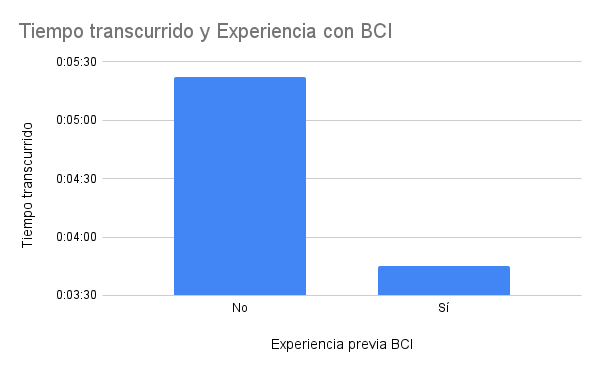
\includegraphics[width=0.7\linewidth]{figures/grafica-Tiempo transcurrido y Experiencia con BCI.png}
   \caption{Gráfica con el tiempo transcurrido y si tenía experiencia previa con el BCI}
   \label{figure:timeelapsedandpreviousexperience}
\end{figure}

\begin{figure}[!htb]
   \centering
    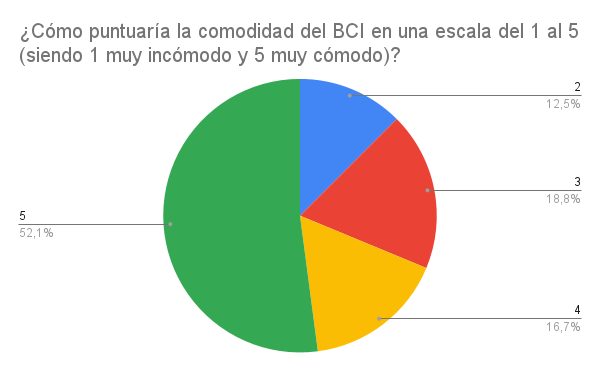
\includegraphics[width=0.7\linewidth]{figures/grafica-¿Cómo puntuaría la comodidad del BCI en una escala del 1 al 5 (siendo 1 muy incómodo y 5 muy cómodo)_.png}
   \caption{Comodidad del BCI}
   \label{figure:comfortableexperience}
\end{figure}


\section{Análisis de los datos}
A pesar de que la muestra es relativamente pequeña, se pueden extraer conclusiones significativas.



Primero, se observó que el cabello no parece influir en la calibración ni en la destreza general del BCI.



En los entornos interiores, la variación entre las calibraciones es mínima, como se puede ver en la Figura \ref{figure:calibrationandtestenvironment}.



Por otro lado, se realizaron pruebas en exteriores bajo las peores condiciones, en pleno sol a mediodía. Los resultados fueron sorprendentes. Si la persona es capaz de ver el estímulo visual (NeuroTags), el NextMind es capaz de reconocerlo sin demasiada dificultad. Se probó con el tutor, quien suele obtener un 5 en la calibración: obtuvo un 4 en la prueba y presentó tiempos de respuesta similares a los obtenidos en interiores.



El tipo de pantalla utilizada al aire libre es un factor que influye considerablemente en los resultados. Se observaron diferencias notables al utilizar pantallas más oscuras, como la mostrada en la figura \ref{figure:entorno-prueba-exterior}, en comparación con pantallas de brillo alto\ref{figure:aplicacion-exterior}. Entre las dos pantallas LCD evaluadas, la que presentaba mayor brillo incorporaba tecnología IPS, a diferencia de la otra. Además, es relevante mencionar que el brillo de las pantallas LCD puede verse afectado por la degradación con el paso del tiempo, teniendo en cuenta que ambas pantallas son LCD, una es nueva mientras que la otra tiene ya 4 años de uso, lo cual podría explicar algunas de las diferencias observadas.



La pantalla utilizada finalmente para la prueba en exterior fue un monitor SAMSUNG F24T350FHU dada por el profesorado.



Además, se encontró que cuanta más calibración se realice, más probabilidades hay de completar la prueba con éxito. Incluso con una calificación de 2, se consideró posible realizar la prueba. Solo en 1 de los 16 casos, la prueba no se pudo realizar con una calibración de 2. Ver Figura \ref{figure:calibrationanddothetest}.



Se observa una correlación aparente entre el tiempo de realización de la prueba y la calificación de calibración: a mayor calificación, menor tiempo necesario para completar la prueba (Figura \ref{figure:timeelapsedandcalibration}).



Es relevante señalar que si los participantes tienen experiencia previa con el uso de BCI, tienden a completar la prueba en menos tiempo (Figura \ref{figure:timeelapsedandpreviousexperience}).



Incluso durante la prueba, se observó una mejora continua en los participantes, independientemente de si su calificación de calibración inicial no era de 4 o 5.



También se consultó a los usuarios sobre su percepción de la comodidad del BCI. Como se aprecia en el gráfico \ref{figure:comfortableexperience}, la mayoría de los usuarios, más del 50\%, calificaron su experiencia como "Muy cómoda", asignándole un 5, el puntaje máximo. En contraste, solo un pequeño grupo, el 12,5\%, le dio un 2, señalando una experiencia de comodidad reducida. Es importante resaltar que ningún usuario otorgó la puntuación mínima de 1, que representaría una experiencia "Muy incómoda".

\section{Adaptación a un nuevo sistema}

La aplicación de Unity ha sido eficientemente adaptada a un nuevo dispositivo: un robot móvil. Este proceso ha puesto de relieve la notable adaptabilidad de la aplicación. Esta capacidad quedó patente cuando logramos recrear una nueva interfaz desde cero, reutilizando los scripts y prefabs existentes, en un plazo de menos de dos horas.



El entorno donde se llevó a cabo esta prueba se puede observar en la figura \ref{figure:entorno-prueba-robot}.

\begin{figure}[!htb]
   \centering
    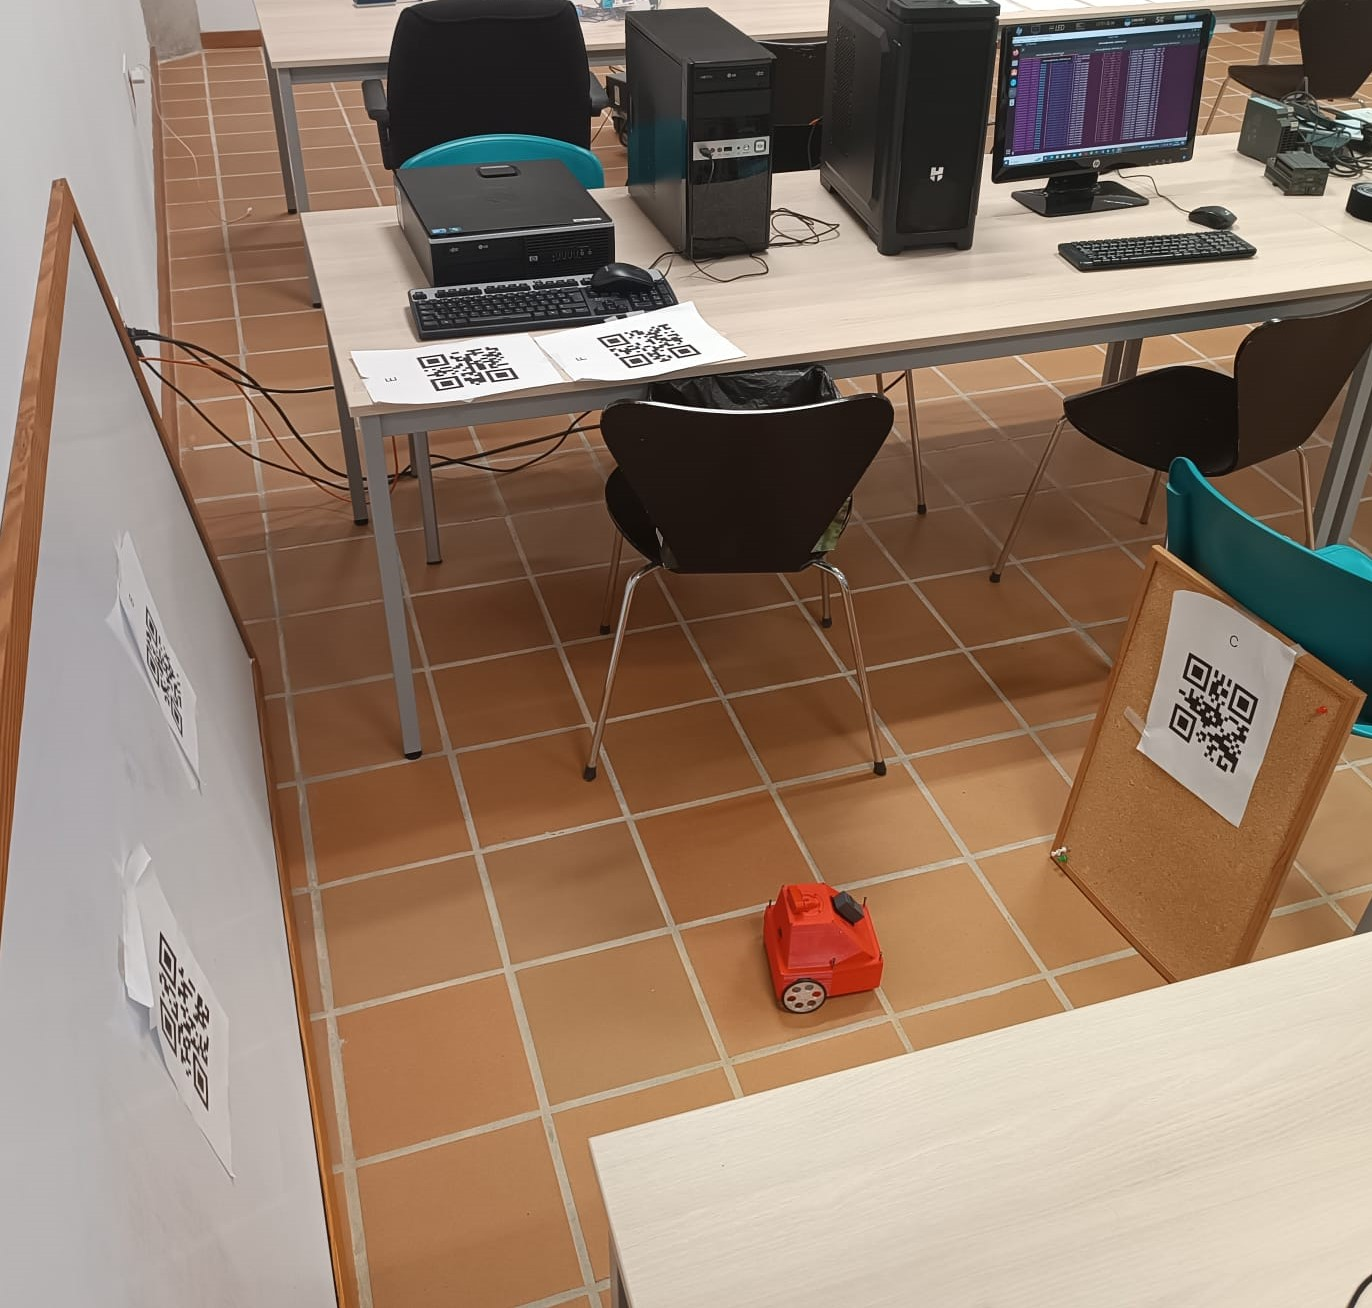
\includegraphics[width=0.6\linewidth]{figures/entorno-prueba-robot.jpg}
   \caption{Entorno de la prueba del robot}
   \label{figure:entorno-prueba-robot}
\end{figure}


\section{Conclusiones}

Este estudio revela la efectividad y versatilidad de NextMind en diversas condiciones y contextos. El dispositivo NextMind demuestra ser un BCI accesible para una amplia variedad de usuarios, sin ser afectado por factores como la presencia de cabello. Muestra una robustez considerable, funcionando de manera efectiva tanto en ambientes interiores como exteriores. Adicionalmente, el rendimiento del dispositivo parece ser casi inmune a las variaciones de luz ambiental, lo cual es un hallazgo que puede orientar el desarrollo futuro de dispositivos BCI. Además, la eficiencia de NextMind tiende a mejorar con una calibración de mayor precisión y con la experiencia previa con dispositivos BCI, lo que destaca la importancia de familiarizarse con esta tecnología. En términos de comodidad, más del 50\% de los usuarios encontraron que NextMind era "Muy cómodo", lo que sugiere una alta aceptabilidad y potencial para su uso continuado.



Para concluir, la interfaz ha demostrado una notable capacidad para adaptarse a diversos contextos y sistemas. Esta flexibilidad refuerza su utilidad, al permitir que se aplique de manera efectiva en una amplia gama de situaciones, haciendo que la interfaz sea una herramienta versátil y eficiente en el campo de la robótica.



%%%%%%%%%%%%%%%%%%%%%%%%%%%%%%%%%%%%%%%%%%%%%%%%%%%%%%%%%
\newpage{\pagestyle{empty}}
\thispagestyle{empty}

\chapter{\LARGE Problemas y dificultades encontradas}
\label{chapter:challengesanddifficulties}

\section{Compatibilidad de versiones}
Dentro del complejo escenario de trabajo que implica la utilización de múltiples herramientas, librerías y tecnologías que no han sido diseñadas a la medida para su integración, emergen frecuentes problemas de incompatibilidad de versiones. Este entorno puede producir desafíos significativos, particularmente cuando las versiones no son compatibles entre sí, generando problemas y retrasos en el desarrollo. Uno de los casos más destacados de esta situación fue el relacionado con UnityRoboticsHub, que se detalla al final de este cap\'itulo.

\section{Chocolatey}
Durante el intento de instalaci\'on de ROS2 para Windows surgieron algunos obstáculos Tras numerosas dificultades, se identificó que la raíz del problema se encontraba en Chocolatey, la herramienta de gestión de paquetes utilizada. La dificultad surgió debido a que Chocolatey no desinstalaba correctamente los paquetes. Este inconveniente requirió una solución manual, que implicó la eliminación de los paquetes directamente en el editor de registros de Windows. Esta tarea, aunque solucionó el problema, destacó la necesidad de herramientas de gestión de paquetes más eficientes y confiables.

\section{Configuración del WiFi: usbipd}
Uno de los desafíos surgió en la configuración del WiFi utilizando usbipd. La dificultad principal se centró en la falta de conciencia de la necesidad de una red estable. El WiFi del ESP32 solo era visible mientras el agente de microros estaba en funcionamiento. Además, se observó que al conectarse al WiFi del ESP32, este se desconectaba y el WiFi se apagaba nuevamente. La causa de este problema radicaba en que la gestión del WiFi se realizaba dentro de la tarea de microros en el microcontrolador. Al cambiar de red, usbipd desconectaba los puertos, provocando problemas en Linux con la existencia de puertos simulados. Esto ocasionaba que el agente de microros dejara de funcionar y, por consiguiente, la tarea de microros dejara de ejecutarse, terminando con la gestión del WiFi.



La solución a este problema consistió en colocar la gestión del WiFi fuera de la tarea de microros. Sin embargo, esto conllevó la desventaja de que el WiFi ya no podía ser controlado desde ROS2.

\section{Inclusi\'on de im\'agenes de la cámara en Unity}
El proceso de introducir la imagen de la cámara en Unity también presentó numerosos problemas. La fuente de la dificultad residía en que se estaba transmitiendo un flujo constante de paquetes MJPEG, que son imágenes. Inicialmente, se intentó utilizar assets de videos y assets de gestión de HTTP en Unity, pero estos enfoques no dieron resultados satisfactorios. La única solución viable consistió en dividir los paquetes y procesarlos para que Unity pudiera visualizarlos a medida que llegaban. Gracias al código abierto que se encontró, fue posible implementar esta parte del proyecto.

\section{Trabajo de cambios}
En términos generales, este proyecto ha estado caracterizado por la necesidad de realizar muchos cambios y adaptaciones en función de las circunstancias que surgían. Aunque este proceso ha sido desafiante, al final se han podido superar todas las adversidades, demostrando la capacidad de adaptación y resiliencia frente a las dificultades.


\section{Imposibilidad de usar ciertos dispositivos}
Inicialmente, se contempló la posibilidad de utilizar una silla de ruedas, lo que llevó a adaptar una interfaz específica para este propósito. Sin embargo, este plan tuvo que ser desechado debido a la falta de disponibilidad de sillas de ruedas robotizadas funcionales en la universidad. Posteriormente, se intentó utilizar un robot, pero este enfoque también resultó fallido debido a problemas en su sistema electrónico.


\section{La persistencia de datos en Unity}
El manejo de la persistencia de datos en Unity presentó una serie de desafíos significativos. Uno de los principales problemas radicó en entender cómo funcionaban los cambios de escena dentro de esta plataforma. En ocasiones, estos cambios resultaban en fallos inesperados y difíciles de rastrear. Adicionalmente, hubo dificultades al tratar de mantener ciertos elementos persistentes, ya que en algunos casos se mantenían más elementos de los planificados. Estos problemas se originaron por una comprensión insuficiente de cómo funciona la persistencia en Unity y cómo se debe manejar un script dentro de un GameObject de forma correcta. A pesar de la cantidad considerable de tiempo perdido en estos asuntos, finalmente se logró obtener un resultado satisfactorio.
\section{Experiencia con Unity-Robotics-Hub}

Unity-Robotics-Hub fue la primera librería que se evaluó para ser utilizada para integrar ROS2 en Unity. Esta librería mostraba signos de robustez y de amplia utilización, lo cual indicaba que podía ser una opción viable.



No obstante, se encontraron serios problemas, ya que la librería presentaba fallos desde las versiones tempranas del código. Existe la posibilidad de que estos problemas se deban a algún tipo de incompatibilidad con la SDK de NextMind.



Se intentaron múltiples soluciones, como la modificación completa del código y el análisis de los registros de Unity. También se probaron las implementaciones de NextMind SDK y UnityRoboticsHub de manera independiente, observando que funcionaban correctamente por separado, pero no conjuntamente.



Es una lastima que Unity-Robotics-Hub no haya funcionado de manera óptima, ya que, a pesar de funcionar a través de un intermediario, el código resultante era más legible y la carga para Unity no era tan elevada como con la implementación actual, que debe manejar ROS2 en su totalidad, generando nodos dentro de Unity.


%%%%%%%%%%%%%%%%%%%%%%%%%%%%%%%%%%%%%%%%%%%%%%%%%%%%%%%%%
\newpage{\pagestyle{empty}}
\thispagestyle{empty}

\chapter{\LARGE Conclusiones y líneas futuras}
\label{chapter:Resultados}

\section{Conclusión}


\section{Líneas futuras}


%%%%%%%%%%%%%%%%%%%%%%%%%%%%%%%%%%%%%%%%%%%%%%%%%%%%%%%%%
\newpage{\pagestyle{empty}}
\thispagestyle{empty}

\chapter{\LARGE Summary and Conclusions}
\label{chapter:Conclusiones}

\section{Conclusions}

In this section, we will discuss the conclusions.

Firstly, I have to highlight that all objectives have been met, although not everything went as expected.

\subsection{Prototype development}
As pointed out in chapter \ref{chapter:challengesanddifficulties}, the need to learn ROS from scratch represented a significant commitment of time and autonomous effort for understanding and assimilating information. Additionally, I had no previous experience programming in Unity, which also implied a learning process from scratch. Regarding specific programming on the ESP32, although it was unknown territory, I benefited from previous knowledge acquired in a degree course called Embedded Systems, which provided a solid foundation for general programming in microcontrollers. This was particularly useful during the programming of the pan-tilt from the microcontroller with respect to PWM, a task that, although it required some research, was simpler thanks to the skills acquired in that subject. Of all aspects of the project, what presented the least complications was the operation of the Neurotags and the NextMind system itself.

In terms of my personal perception of the tools used, I found ROS fascinating and it is a tool I would like to continue using in the future. My experience with Unity, on the other hand, was not as positive due to its logging and error management system, which I consider complicated to locate faults. As for ESP-IDF, it provided me with a satisfactory experience, perceiving it as a more modular structure than a micro-ROS project for Freertos microcontroller programming.

\subsection{Interpretation of data and conclusions obtained}
 
The results of the study point to the effectiveness and adaptability of NextMind in different environments and situations. As a BCI, it is accessible and resilient, not being influenced by aspects such as the presence of hair. Its efficient performance, both indoors and outdoors, and its resistance to variations in ambient light, open up new possibilities for future advances in BCI devices. It was observed that precise calibration and prior experience with BCIs improve its efficiency, underlining the need for familiarization with the technology. As for comfort, most users rated NextMind positively, indicating its potential for extended use.

\section{Future lines}

\subsection{Prototype improvements}

With a view to continuing the development and improvement of the project, various possible actions and modifications have been identified to improve its operation and expand its utility.

\begin{itemize}

\item \textbf{Improve the camera}: The camera's resolution could be improved to more clearly capture the QR codes. A more powerful camera would contribute to improving the effectiveness and precision in the detection of the codes.

\item \textbf{Implement an undo state function}: It would be useful to incorporate a function in the prototype to quickly reverse the state of the camera within the QR detection, for example, through a button or a key on the keyboard that allows removing a state in a simple way.

\item \textbf{Improvements in calibration and adjustment of the device}: According to the opinions collected, the device in general is not difficult to put on, but some people with certain types of hair may have difficulties. Therefore, options could be explored to facilitate its adjustment. In addition, it could be beneficial to have an alternative method for calibration in case of failure.

\item \textbf{Incorporate acoustic feedback}: Some users, apparently, were so focused on the stimulus that they did not notice the visual feedback provided by the NeuroTag. To facilitate the user's perception, an additional acoustic stimulus could be added to the visual one.

\item \textbf{Expand controls with NeuroButtons}: It would be convenient to implement numbered NeuroButtons from 1 to 5, where each number represents a specific amount of automatic movements that the Pan-Tilt system can perform.

\item \textbf{Explore more devices}: The application of the BCI can be expanded to other devices, such as a robotic chair or a robot, which would open new possibilities for remote control of various devices through the brain-computer interface.

\end{itemize}


\subsection{Research improvements}

\begin{itemize}
\item \textbf{Expand the sample}: A larger sample will allow for more representative and reliable results in tests, and more accurate conclusions can be drawn.

\item \textbf{Explore the impact of ambient noise}: Considering that this prototype is designed for outdoor use, it would be interesting to study how difficulty concentrating in noisy environments can affect the performance of NextMind. This could involve conducting more tests in these contexts.

\item \textbf{Investigate the effect of ADHD}: Studying the effects of Attention Deficit Hyperactivity Disorder (ADHD) on the use of NextMind can provide useful insights as concentration is vital in this BCI.

\item \textbf{Study the adaptation to the device in people with visual conditions}: 
During the tests, certain patterns were found, although not enough, between visual conditions and score in calibration. The study of how people with different visual conditions (myopia, astigmatism, hypermetropia, etc.) adapt to the use of NextMind could be interesting.

\item \textbf{Analyze the effect of prolonged training}:

 Investigate if the effectiveness of the device can improve with practice and prolonged training and determine the time needed to observe significant improvements. As during the tests, clear indications were seen that having previous experience in the use of BCI resulted in better mastery of it.

\item \textbf{Study the effect of fatigue}: Investigate how fatigue or mental tiredness can affect the performance of NextMind. This could help determine how long it can be effectively used before fatigue begins to affect performance.

\end{itemize}

%%%%%%%%%%%%%%%%%%%%%%%%%%%%%%%%%%%%%%%%%%%%%%%%%%%%%%%%%
\newpage{\pagestyle{empty}}
\thispagestyle{empty}

\chapter{\LARGE Presupuesto}
\label{chapter:presupuesto}


\section{Presupuesto}

\begin{table}[htb]
\centering
\resizebox{\textwidth}{!}{%
\begin{tabular}{l|l|l|l|}
\hline
\multicolumn{1}{|l|}{Concepto}                                                                                                          & Coste por horas & Horas & Coste total \\ \hline
\multicolumn{1}{|l|}{Documentación}                                                                                                     & 20              & 60    & 1200€       \\ \hline
\multicolumn{1}{|l|}{Diseño de la base de datos}                                                                                        & 20              & 50    & 1000€       \\ \hline
\multicolumn{1}{|l|}{Implementación de mejoras en la interfaz de usuario}                                                               & 20              & 90    & 1800€       \\ \hline
\multicolumn{1}{|l|}{Implementación de mejoras en la API}                                                                               & 20              & 70    & 1400€       \\ \hline
\multicolumn{1}{|l|}{\begin{tabular}[c]{@{}l@{}}Implementación de la base de datos y \\ adaptación del servicio de docker\end{tabular}} & 20              & 40    & 800€        \\ \hline
\multicolumn{1}{|l|}{\begin{tabular}[c]{@{}l@{}}Desarrollo de funcionalidades para\\ administradores (Script y panel)\end{tabular}}     & 20              & 35    & 700€        \\ \hline
                                                                                                                                        & Total           & 345   & 6900€       \\ \cline{2-4} 
\end{tabular}%
}
\caption{Presupuesto del proyecto}
\end{table}



%%%%%%%%%%%%%%%%%%%%%%%%%%%%%%%%%%%%%%%%%%%%%%%%%%%%%%%%%
\newpage{\pagestyle{empty}}
\thispagestyle{empty}

\chapter{\LARGE Bibliografía}
\label{chapter:Bibliografía}

%
%
\begingroup
\renewcommand{\section}[2]{}
\renewcommand{\chapter}[2]{}
\bibliographystyle{apalike}
\bibliography{memtfg.bib}
\endgroup

%%%%%%%%%%%%%%%%%%%%%%%%%%%%%%%%%%%%%%%%%%%%%%%%%%%%%%%%%%

%\begin{thebibliography}{X}
% Aquí figurará la bibliografía
%\end{thebibliography}

%%%%%%%%%%%%%%%%%%%%%%%%%%%%%%%%%%%%%%%%%%%%%%%%%%%%%%%%%

\newpage{\pagestyle{empty}\cleardoublepage}
\thispagestyle{empty}

\begin{appendix}

\chapter{\LARGE Preparación del entorno de desarrollo}
\label{appendix:1}
En este apéndice, se detallará la configuración del entorno de desarrollo utilizado para este proyecto. El ecosistema de desarrollo se compone principalmente de Unity, el middleware ROS, y la librería Ros2ForUnity. Se explicarán los pasos necesarios para instalar y ajustar cada uno de estos componentes para asegurar un funcionamiento óptimo. Por último se explicará el funcionamiento y la experiencia tenida con otra librería llamada Unity-Robotics-Hub.


\section{NextMind SDK}

\subsection{Requerimientos del SDK}
Para poder usar el SDK de NextMind es importante tener en cuenta que tiene una serie de requerimientos que se muestran a continuación:

\subsubsection{Requisitos mínimos de hardware}
\begin{itemize}
  \item Soporte Bluetooth LE (4.0)
  \item Gráficos - DX9 shader model 2.5, equivalente a Intel HD 2500
  \item CPU - Intel i5-4590, equivalente a AMD FX 8350
  \item RAM - 8 GB
\end{itemize}

\subsubsection{Compatibilidad de software}
\begin{itemize}
  \item Última versión probada: Unity - 2022LTS
  \item Versión oficial soportada: Unity - 2020LTS, 2019LTS
  \item Plataformas - Windows 10 de 64 bits, Apple macOS de 64 bits (Mojave, Catalina, Big Sur)
  \item Software probado y aprobado - Oculus Rift, Oculus Quest 1 y 2, HTC Vive y Pro, HoloLens 1
  \item Compatibilidad de software verificada - Valve Index, HoloLens 2
\end{itemize}

\subsection{Instalación del SDK}

La instalación del NextMind SDK es un proceso sencillo que se realiza a través de la plataforma Unity. En primer lugar, es necesario descargar el SDK desde el sitio web oficial de NextMind o directamente desde el Unity Asset Store. Tras la descarga, el SDK puede ser importado al proyecto de Unity utilizando el menú ``Assets''.

\subsection{Desarrollo con el SDK}

Con el SDK correctamente instalado, ahora se puede comenzar a desarrollar aplicaciones que interactúan con el dispositivo NextMind. La documentación del SDK proporciona una serie de tutoriales y ejemplos que pueden ayudar a comenzar.
\section{ROS 2}
La librería Ros2ForUnity requiere la instalación de ROS 2 en Windows (Windows 10), así como en el Subsistema de Windows para Linux (WSL), específicamente Ubuntu 22.04.2 LTS. Aunque no todas las librerías exigen la instalación de ROS2 en Windows, para Ros2ForUnity es imprescindible si tenemos Unity en Windows, como es el caso.

\subsection{Instalación de ROS 2 en Ubuntu}
Se optó por la versión Humble de ROS 2 para Ubuntu, siguiendo las instrucciones proporcionadas en la documentación oficial\footnote{ROS Humble Installation Ubuntu: \url{https://docs.ros.org/en/humble/Installation/Alternatives/Ubuntu-Development-Setup.html}}. Después de la instalación, se llevaron a cabo varias pruebas para confirmar que todo funcionaba correctamente, como se puede ver en la Figura \ref{figure:ros2-examples-installation-Ubuntu}.

\begin{figure}[ht]
   \centering
    \includegraphics[width=0.8\linewidth]{figures/prueba instalación ros2.png}
   \caption{Ejemplos de funcionamiento de la instalación de ROS 2 Ubuntu}
   \label{figure:ros2-examples-installation-Ubuntu}
\end{figure}

\subsection{Instalación de ROS 2 en Windows 10}
Para instalar ROS 2 en Windows 10, se siguió la documentación oficial de ROS 2 Humble\footnote{ROS Humble Installation Windows: \url{https://docs.ros.org/en/humble/Installation/Alternatives/Windows-Development-Setup.html}}. Se recomienda realizar la instalación desde la PowerShell con privilegios de administrador. Dado que el comando ``call'' no está disponible en PowerShell, se sustituyó por:

\begin{verbatim}
C:\dev\ros2\_humble\local\_setup.ps1
\end{verbatim}



Es importante tratar con cuidado a Chocolatey, ya que puede tener dificultades para desinstalar completamente los paquetes que instala. Si se produce un error, será necesario eliminar los paquetes manualmente a través del editor de registros de Windows.



Finalmente, es crucial prestar atención a las versiones de .Net y al Visual Studio 2019. Visual Studio 2019, se debe asegurar que no se instalan las herramientas C++ CMake, deseleccionándolas en la lista de componentes a instalar.

\section{ESP-IDF}
Para poder instalar el ESP-IDF release 5.1 de Linux en ESP32, se necesita instalar el siguiente software:

\begin{itemize}
  \item Conjunto de herramientas de compilación para el ESP32.
  \item Herramientas de construcción: CMake y Ninja, para construir una aplicación completa para ESP32.
  \item ESP-IDF, que contiene esencialmente la API (bibliotecas de software y código fuente) para ESP32, así como scripts para operar el conjunto de herramientas.
\end{itemize}

\subsection{Instalación de ESP-IDF}
La instalación del ESP-IDF se debe llevar a cabo siguiendo las instrucciones de su documentación oficial\footnote{ESP-IDF Get Started Guide: \url{https://docs.espressif.com/projects/esp-idf/en/latest/esp32/get-started/}}. La versión instalada en este proyecto es la release 5.1.



Aunque la documentación del ESP-IDF proporciona instrucciones de instalación para varios sistemas operativos, en este proyecto se decidió instalarlo en Linux. Esta decisión se tomó en las etapas iniciales del proyecto, incluso antes de considerar el uso de ROS 2 en Windows. En consecuencia, toda la gestión del ESP32 se realiza desde Linux, aprovechando la instalación existente de ROS 2 en la WSL.



Además, cabe destacar que micro-ROS no proporciona instrucciones para su instalación en Windows y no se puede garantizar que el proceso de compilación funcione correctamente en ese sistema operativo. Esto también influenció la elección de utilizar Linux para el desarrollo del proyecto.

\subsection{Consideraciones con la WSL}
\label{WLS-considerations}
Es importante tener en cuenta que los puertos USB están gestionados por el sistema operativo Windows. Para hacerlos accesibles desde la WSL, se utilizó el programa usbipd\footnote{USBIPD-WIN project: \url{https://learn.microsoft.com/en-us/windows/wsl/connect-usb}} en Windows. Primero, se listan los puertos USB conectados para obtener el BUSID con el siguiente comando:

\begin{verbatim}
usbipd wsl list
\end{verbatim}

Luego, se ejecuta el siguiente comando para ``atar'' el puerto USB a la WSL:

\begin{verbatim}
usbipd wsl attach --busid (busid)
\end{verbatim}

Los puertos en sistemas Linux se ubican en el directorio \textbf{/dev/} y suelen tener nombres del tipo \texttt{ttyUSBX}, donde X es un número entero positivo.



Es necesario otorgar permisos de lectura y escritura al puerto para su uso. Para ello, se puede utilizar el siguiente comando:

\begin{verbatim}
sudo chmod a+rw /dev/ttyUSBX
\end{verbatim}

En este comando, es importante reemplazar \texttt{ttyUSBX} con el nombre del puerto que se desea utilizar.

\subsection{Creación de componentes}
\label{subsection:componentcreation}

\textbf{Requisitos para la creación componentes:}
\begin{enumerate}
\item \textbf{Modularidad:} Ser una unidad funcionalmente independiente y cohesiva.
\item \textbf{Reutilización:} Ser capaz de utilizarse en diferentes contextos y proyectos.
\item \textbf{Interfaz bien definida:} Especificar cómo interactuar con el componente.
\item \textbf{Encapsulación:} Ocultar los detalles internos de implementación y proporcionar una interfaz de alto nivel.
\item \textbf{Independencia:} No depender directamente de otros componentes.
\item \textbf{Coherencia y cohesión:} Tener una estructura y diseño coherentes, así como una funcionalidad interna relacionada.
\item \textbf{Testeabilidad:} Ser fácil de probar de forma unitaria y escribir pruebas automatizadas.
\item \textbf{Documentación:} Estar debidamente documentado con información relevante.
\end{enumerate}

En el contexto de ESP-IDF, añadir un componente es tan sencillo como ponerlo en el directorio de components.

Para que se añada correctamente hay que añadir en el CMakeLists.txt de fuera lo siguiente:

\begin{lstlisting}[label={lst:CMakeLists-extern-ESP-IDF}, caption=CMakeLists del repositorio ESP-IDF]
cmake_minimum_required(VERSION 3.5)

set (EXTRA_COMPONENT_DIRS "components/")

include($ENV{IDF_PATH}/tools/cmake/project.cmake)
project(pan-tilt-esp32)
\end{lstlisting}

Luego dentro de cada componente hay que tener otro CMakeLists.txt con lo siguiente:
\begin{lstlisting}[label={lst:CMakeLists-component-ESP-IDF}, caption=CMakeLists del componente ESP-IDF]
idf_component_register(
    SRCS "script1.c" "script2.c"
    INCLUDE_DIRS "."
    REQUIRES <alguna dependencia>
)
\end{lstlisting}

También se le puede añadir un directorio de test para testear el componente usando U-TTS.



Dentro de ese directorio debe haber otro CMakeLists.txt:
\begin{lstlisting}[label={lst:CMakeLists-component-tests}, caption=CMakeLists de los tests del componente]
idf_component_register(SRC_DIRS "."
                    INCLUDE_DIRS "."
                    REQUIRES <nombre del componente> unity)
\end{lstlisting}

Luego al mismo nivel en el directorio debe haber un fichero con los tests incluyendo la librería de U-TTS y el nombre del componente a testear:

\begin{verbatim}
#include "unity.h"
\end{verbatim}



\subsection{Componente de micro-ROS}
\label{subsection:microroscomponent}

Como se mencionó anteriormente, en el marco de trabajo con ESP-IDF, MicroROS se añade como un componente\footnote{Micro-ROS Component: \url{https://github.com/micro-ROS/micro_ros_espidf_component}}. Este componente ha sido validado en las versiones ESP-IDF v4.3, v4.4 y v5.0, siendo compatible con ESP32, ESP32-S2, ESP32-S3 y ESP32-C3.

\subsubsection{Dependencias}

Para el correcto funcionamiento de este componente, es necesario instalar \textbf{colcon} y otros paquetes de Python 3 dentro del entorno virtual de IDF, para la construcción de paquetes de micro-ROS:

\begin{verbatim}
. $IDF_PATH/export.sh
pip3 install catkin_pkg lark-parser empy colcon-common-extensions
\end{verbatim}

\subsubsection{Middlewares disponibles}

El componente de micro-ROS permite trabajar con dos middlewares diferentes:

\begin{itemize}
\item \textbf{eProsima Micro XRCE-DDS:} Este es el middleware predeterminado de micro-ROS. XRCE-DDS es un protocolo diseñado para permitir comunicaciones eficientes y efectivas entre clientes y agentes en sistemas embebidos, siendo por tanto adecuado para entornos con recursos limitados.

\item \textbf{EmbeddedRTPS:} Se trata de una implementación experimental de un middleware RTPS compatible con ROS 2. El middleware RTPS (Real-Time Publish-Subscribe) es un protocolo de capa de middleware que proporciona comunicación en tiempo real en redes de área amplia. Este middleware se utiliza en sistemas distribuidos y entornos de tiempo real.
\end{itemize}

Para seleccionar uno de estos middlewares, se debe usar el comando \textbf{idf.py menuconfig} y acceder a \textbf{micro-ROS Settings > micro-ROS middleware}.



En el presente proyecto, se optó por el uso del middleware predeterminado, eProsima Micro XRCE-DDS.

\subsubsection{Instalación del componente}

El componente de MicroROS puede incorporarse al proyecto ESP-IDF clonando directamente el repositorio correspondiente en el directorio \textbf{components}. Es importante destacar que la rama a clonar del repositorio debe coincidir con la versión de ROS2 que se está utilizando. En el contexto de este proyecto, dado que se está utilizando ROS2 Humble, se ha clonado la rama ``Humble'' del repositorio.



En caso de enfrentar dificultades durante el proceso de compilación, es recomendable verificar que se está operando en un entorno de shell limpio, es decir, sin que el script de configuración de ROS 2 esté en funcionamiento.

\subsection{Guía de uso}
\label{subseccion:usageespidf}
Esta sección presenta una guía paso a paso para poner en marcha el proyecto:

\begin{itemize}
\item Ejecutar el comando \texttt{idf.py set-target esp32} para seleccionar el microcontrolador ESP32 como objetivo.
\item Configurar el proyecto ejecutando \texttt{idf.py menuconfig}.
\item Construir el proyecto con \texttt{idf.py build}.
\item Conectar el dispositivo y luego cargar el proyecto en el dispositivo con el comando \texttt{idf.py -p PORT flash}, sustituyendo \texttt{PORT} por el puerto correspondiente del dispositivo.
\item Monitorear la salida de la aplicación con \texttt{idf.py -p PORT monitor}.
\end{itemize}

Es importante reemplazar \texttt{PORT} con el puerto apropiado para su sistema teniendo en cuenta lo visto en el apartado \ref{WLS-considerations}.


\section{Agente de micro-ROS}
\label{section:microrosagent}

El agente de micro-ROS es un componente fundamental del framework de micro-ROS. Sirve de intermediario entre los nodos de micro-ROS en el microcontrolador y los nodos de ROS2 en el sistema del ordenador. En este caso particular, se ejecutará micro-ROS en Linux a través de la WSL. Para lograr esto, utiliza la implementación eProsima Micro XRCE-DDS del protocolo DDS para conectar las funcionalidades de micro-ROS con las funcionalidades más extensas de ROS2 \cite{MicroXRCE-DDS2023}.

Existen varias formas de ejecutar el agente de micro-ROS, dos de las cuales se detallan a continuación:

\subsection{Usando un repositorio de micro-ROS}

Una opción para ejecutar el agente de micro-ROS es a través de un repositorio de micro-ROS. La instalación de dicho repositorio se realiza de manera sencilla siguiendo los primeros pasos del tutorial oficial de micro-ROS\footnote{First micro-ROS Application on Linux: \url{https://micro.ros.org/docs/tutorials/core/first_application_linux/}}.

Para ejecutar el agente, se utiliza la utilidad \textit{micro\_ros\_agent} incluida en el repositorio:

\begin{verbatim}
ros2 run micro_ros_agent micro_ros_agent [transport] [options]
\end{verbatim}

El parámetro [transport] especifica el tipo de transporte utilizado para la comunicación (por ejemplo, udp, serial, etc.). Los [options] son argumentos adicionales específicos del tipo de transporte seleccionado.

Por ejemplo, el siguiente comando utiliza una comunicación serial a través del dispositivo \texttt{/dev/ttyUSB0}:

\begin{verbatim}
ros2 run micro_ros_agent micro_ros_agent serial /dev/ttyUSB0
\end{verbatim}

Para ejecutar cualquier comando de ROS2, es necesario inicializar previamente el entorno de ROS2.

\subsection{Uso de Docker para ejecutar el agente de micro-ROS}

Alternativamente, es posible utilizar Docker para ejecutar el agente de micro-ROS. Inicialmente, se debe iniciar el daemon de Docker con el siguiente comando:

\begin{verbatim}
sudo dockerd
\end{verbatim}

Posteriormente, hay que ejecutar el agente de micro-ROS utilizando el siguiente comando:

\begin{verbatim}
sudo docker run -it --rm -v /dev:/dev --privileged --net=host
microros/micro-ros-agent:humble serial --dev /dev/ttyUSB0 -v6
\end{verbatim}

Este comando ejecuta el agente de micro-ROS dentro de un contenedor Docker, otorgándole acceso a los dispositivos del sistema anfitrión y configurando la red del contenedor para utilizar la red del sistema anfitrión. En este caso, se está utilizando el agente de micro-ROS para la versión ``humble'' de ROS, utilizando una conexión serial a través del dispositivo \texttt{/dev/ttyUSB0}.

\begin{figure}[ht]
   \centering
    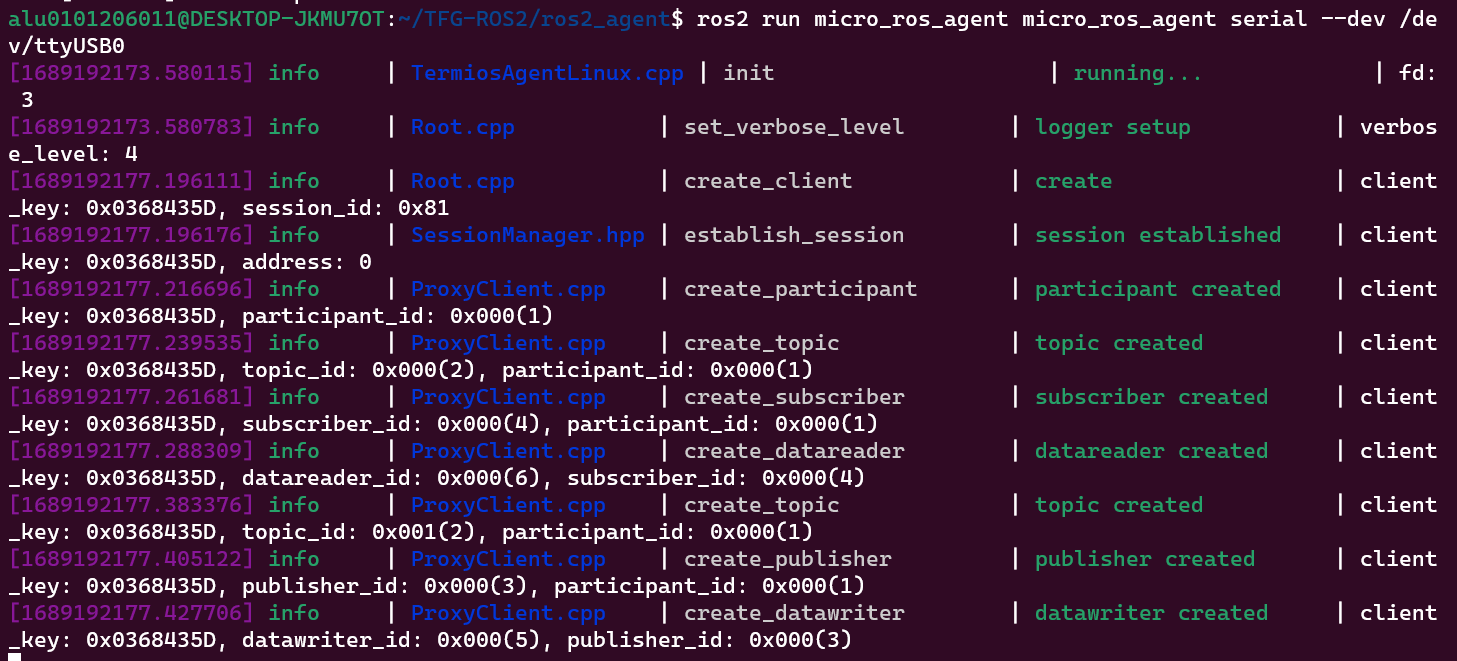
\includegraphics[width=1\linewidth]{figures/ros-agent.png}
   \caption{Ejecución del agente de micro-ROS}
   \label{figure:microrosagent}
\end{figure}


\subsection{Consideraciones adicionales}

El funcionamiento de micro-ROS depende de la ejecución de un programa agente que expone los nodos de ROS2 creados en un microcontrolador de modo que sean visibles para toda la red accesible por ROS2. El agente micro-ROS puede comunicarse con el dispositivo micro-ROS de dos formas: por comunicación serial o mediante el protocolo UDP. En el primer caso, la comunicación entre el programa micro-ROS en el dispositivo y el agente no es problemática porque el programa conecta directamente con el agente con el sistema serial. Sin embargo, si se usa UDP por ejemplo en una red wifi, hay que proporcionar al programa micro-ROS, la dirección y el puerto del agente dentro de esa red. El problema radica en que el subsistema windows de linux no es accesible directamente utilizando la IP asignada por Windows a la interfaz de red virtual creada para WSL. Se puede crear una pasarela para comunicarse con una aplicación en WSL mediante la herramienta netfs, pero bajo el protocolo TCP, y no funciona en la actualidad para el protocolo UDP. La solución para no depender de un ordenador adicional bajo linux, pasaría por utilizar una máquina virtual Virtual box en Windows para ejecutar el agente, ya que este sistema sí admite la creación de un puente con el interfaz de red wifi.

\section{Ros2ForUnity}
\label{ros2forunity}

Ros2ForUnity es una librería de Unity que permite crear nodos de ROS 2 con código C\# de Unity.


\subsection{Instalación de Ros2ForUnity}
Para instalar la librería se han seguido los documentos markdown del repositorio de GitHub del proyecto \footnote{Ros2ForUnity Windows Installation: \url{https://github.com/RobotecAI/ros2-for-unity/blob/develop/README-WINDOWS.md}}. En este proyecto se ha comprobado su funcionamiento hasta el commit:

\begin{verbatim}
3f548920bc4c33e178707a888d01592905bef1e9
\end{verbatim}



Hay que prestar especial atención a los prerequisitos y a los avisos importantes que se señalizan dentro del ``README-WINDOWS.md'' del repositorio. Y en ejecutar la Powershell en modo administrador.



Al momento de construir el proyecto Ros2ForUnity, es necesario seleccionar la versión ``overlay''. Esta elección se debe a que la versión ``standalone'' proporciona una instancia única de ROS dentro de Unity, que no corresponde al comportamiento deseado para este proyecto.



Ahora hay dos opciones para instalar el asset en Unity. Ejecutar el comando siguiente para crear un package e instalarlo en Unity de manera habitual:

\begin{verbatim}
create\_unity\_package.ps1
\end{verbatim}

O copiar y pegar en los assets del proyecto de Unity el directorio que se encuentra en \textbf{install/asset/}.

\subsection{Uso de Ros2ForUnity con ROS2}

Una vez instalado Ros2ForUnity en Unity, es importante recordar que se debe iniciar Unity a través de la terminal después de iniciar ROS2. Esto se debe a que Ros2ForUnity necesita acceso a la instancia de ROS2 que se ejecuta en el sistema para funcionar correctamente.

Primero, se debe iniciar ROS2. Si estás utilizando ROS2 Humble en Windows, puedes hacerlo ejecutando el siguiente comando en PowerShell:

\begin{verbatim}
C:\dev\ros2_humble\local_setup.ps1
\end{verbatim}

Asegúrate de que tu terminal esté en el directorio que contiene tu script de configuración de ROS2 local antes de ejecutar este comando.

Después de haber iniciado ROS2, puedes abrir tu proyecto de Unity a través de la terminal utilizando el comando unity con la opción -projectPath seguido de la ruta a tu proyecto:

\begin{verbatim}
unity.exe -projectPath "D:\Unity\Unity Projects\Thesis-Unity-Pan-Tilt"
\end{verbatim}

Con ROS2 en funcionamiento y Unity abierto de esta manera, deberías ser capaz de utilizar Ros2ForUnity para crear nodos de ROS2 con el código C\# de Unity.


\subsection{Consideraciones}

Es necesario asignar a la variable de entorno ROS\_IP una dirección IP que permita la comunicación entre ROS2 en la WSL y ROS2 en el sistema operativo Windows.

\begin{figure}[!htb]
    \centering
    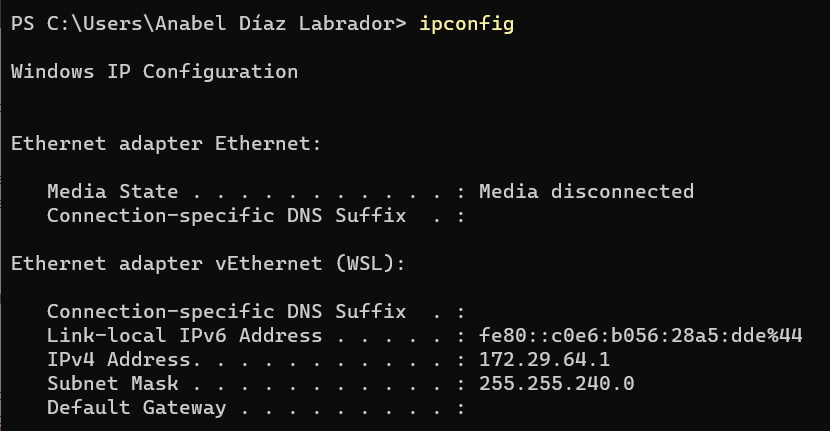
\includegraphics[width=0.8\linewidth]{figures/wsl-network-powershell.png}
    \caption{Red de la WSL visualizada en PowerShell}
    \label{figure:wsl-network-powershell}
\end{figure}



La necesidad de usar la dirección IP de la WSL se origina del hecho de que la comunicación entre la WSL y Windows se realiza a través de una red virtual interna. Esta dirección IP asegura que los mensajes enviados por ROS2 en la WSL sean recibidos por ROS2 en Windows y viceversa. Se puede observar en la figura \ref{figure:wsl-network-powershell}.



Comandos para asignar la dirección IP:



En Windows (usando PowerShell):
\begin{verbatim}
$env:ROS_IP='172.29.67.184'
\end{verbatim}


En WSL:
\begin{verbatim}
export ROS_IP=172.29.67.184
\end{verbatim}
\section{Cámara}

La cámara utilizada es una M5 Stack Timercam, como se menciona en la sección \ref{section:camara}.

\subsection{Instalación del entorno de trabajo}
\label{section:cameraenvironmentinstallation}

El software de la cámara es específico y solo es compatible con la versión ESP-IDF v4.0.1. Para garantizar una correcta instalación, es necesario clonar esta versión específica del repositorio.

\begin{verbatim}
git clone -b v4.0.1 --recursive 
https://github.com/espressif/esp-idf.git esp-idf-v4.0.1
\end{verbatim}

Posteriormente, es necesario instalar el entorno de desarrollo descargado para poder interactuar con él.

\begin{verbatim}
~/esp_idf_4.0/esp-idf-v4.0.1$ ./install.sh
\end{verbatim}

Para poder compilar el código de la cámara o monitorizarla desde la terminal, entre otras acciones, siempre será necesario ejecutar el siguiente comando en el directorio ``~/esp\_idf\_4.0/esp-idf-v4.0.1'':

\begin{verbatim}
source export.sh
\end{verbatim}

Es importante mencionar que no se puede ejecutar este comando después de haber hecho un source export.sh de otro ESP-IDF.

Para facilitar el uso de estos comandos, se han creado los siguientes alias que se deben añadir al archivo .bashrc:

\begin{verbatim}
alias get_idf='. $HOME/esp/esp-idf/export.sh'
alias get_idf4='. $HOME/esp_idf_4.0/esp-idf-v4.0.1/export.sh'
\end{verbatim}



\chapter{\LARGE Códigos relevantes del proyecto}
\label{appendix:2}
\section{Script Don't Destroy On Load}
\label{appendix:dontdestroyonload}

\begin{lstlisting}[label=lst:dontdestroyonload, caption={Código de Don't Destroy On Load}]
using UnityEngine;

public class DontDestroyOnLoad : MonoBehaviour {
  public static DontDestroyOnLoad Instance;

  void Awake() {
    if (Instance == null) {
      Instance = this;
      DontDestroyOnLoad(gameObject);
    } else {
      Destroy(gameObject);
    }
  }
}
\end{lstlisting}


\section{Script Ros2Start.cs}
\label{appendix:ros2startscript}

\begin{lstlisting}[label=lst:Ros2StartCode, caption={Código de Ros2Start}]
using System.Collections;
using System.Collections.Generic;
using UnityEngine;
using ROS2;
using System.Collections.Concurrent;

public class Ros2Start : MonoBehaviour {
  public static Ros2Start Instance { get; private set; }

  private ROS2UnityComponent ros2Unity;
  private ROS2Node ros2Node;
  public IPublisher<std_msgs.msg.Header> action_pub;
  private ISubscription<std_msgs.msg.Header> esp32_sub;

  public delegate void MessageReceivedHandler(std_msgs.msg.Header msg);
  public event MessageReceivedHandler OnMessageReceived;

  // Thread-safe queue for incoming messages
  public ConcurrentQueue<std_msgs.msg.Header> messageQueue = new ConcurrentQueue<std_msgs.msg.Header>();

  // Start is called before the first frame update
  void Start() {
    if (Instance != null) {
      Destroy(gameObject);
      return;
    }
    Instance = this;
    DontDestroyOnLoad(gameObject);

    Debug.Log("Starting ROS2 node");

    ros2Unity = GetComponent<ROS2UnityComponent>();
    if (ros2Unity.Ok()) {
      ros2Node = ros2Unity.CreateNode("ROS2UnityPublisherSubscriberNode");
      Debug.Log("Starting ROS2 node 2");
    } else {
      Debug.Log("Ros2Unity was not created OK");
    }

    if (ros2Unity.Ok()) {
      action_pub = ros2Node.CreatePublisher<std_msgs.msg.Header>("action"); 
      esp32_sub = ros2Node.CreateSubscription<std_msgs.msg.Header>("freertos_header_log", 
        msg => {
          Debug.Log("Unity listener heard: [" + msg.Frame_id + "]");
          messageQueue.Enqueue(msg);
        });
      std_msgs.msg.Header msg = new std_msgs.msg.Header();
      msg.Frame_id = "CON_/CAM";
      Debug.Log(msg.Frame_id);
      action_pub.Publish(msg);
    } else {
      Debug.Log("ROS2UnityComponent was not created OK");
    }
  }


  void Update() {
    while (messageQueue.TryDequeue(out std_msgs.msg.Header msg)) {
        OnMessageReceived?.Invoke(msg);
    }
  }
}
\end{lstlisting}

\section{Script Ros2SubscriberHandler.cs}
\label{appendix:ros2subscriberhandler}

\begin{lstlisting}[label=lst:Ros2SubscriberHandlerCode, caption={Código de Ros2SubscriberHandler}]
using System.Collections;
using System.Collections.Generic;
using UnityEngine;

public class Ros2SubscriberHandler : MonoBehaviour
{
  public static Ros2SubscriberHandler Instance { get; private set; }

  public Ros2Start ros2Subscriber;
  public bool CameraEnabled { get; set; }
  public string CameraIP { get; set; }
  public bool ESP32Enabled { get; set; }

  private void Awake() {
    if (Instance != null) {
      Destroy(gameObject);
      return;
    }
    Instance = this;
    DontDestroyOnLoad(gameObject);
  }

  void Start() {
    CameraEnabled = false;
    CameraIP = "No camera IP";
    ESP32Enabled = false;
  }

  // Manage the event of receiving a message
  void OnEnable() {
    if (ros2Subscriber == null) {
      ros2Subscriber = GetComponent<Ros2Start>();
      if (ros2Subscriber != null) {
        ros2Subscriber.OnMessageReceived += ProcessReceivedMessage;
      }
    } else {
      ros2Subscriber.OnMessageReceived += ProcessReceivedMessage;
    }
  }

  void ProcessReceivedMessage(std_msgs.msg.Header msg) {
    string[] parts = msg.Frame_id.Split(' ');

    if (parts.Length >= 5 && parts[0] == "Target" && parts[1] == "station" && parts[2] == "has" && parts[3] == "ip") {
      CameraEnabled = true;
      CameraIP = parts[4];
      Debug.Log("IP camera: " + CameraIP);
    }

    if (parts.Length >= 3 && parts[0] == "Camera" && parts[1] == "ip:") {
      CameraEnabled = true;
      CameraIP = parts[2];
      Debug.Log("IP camera: " + CameraIP);
    }

    if (parts.Length >= 3 && parts[0] == "Target" && parts[1] == "station" && parts[2] == "disconnected") {
      CameraEnabled = false;
      CameraIP = "No camera IP";
      Debug.Log("Camera disabled");
    }

    if (parts.Length >= 4 && parts[0] == "Wifi" && parts[1] == "init" &&  parts[2] == "softap" && parts[3] == "finished") {
      ESP32Enabled = true;
      Debug.Log("ESP32 enabled");
    }

    if (parts.Length >= 4 && parts[0] == "Stopping" && parts[1] == "WiFi" &&  parts[2] == "in" && parts[3] == "base" && parts[4] == "station") {
      ESP32Enabled = false;
      Debug.Log("ESP32 disabled");
      CameraIP = "No camera IP";
      CameraEnabled = false;
    }
  }
}
\end{lstlisting}


\section{Script Ros2Publish}
\label{appendix:ros2publishscript}

\begin{lstlisting}[label={lst:Ros2PublishCode}, caption={Código de Ros2Publish}]
using System.Collections;
using System.Collections.Generic;
using UnityEngine;
using ROS2;

public class Ros2Publish : MonoBehaviour {
  private Ros2Start ros2Publisher;
  private IPublisher<std_msgs.msg.Header> action_pub;


  void Update() {
    if (ros2Publisher == null) {
      ros2Publisher = Ros2Start.Instance;
    }
  }


  public void OnUpNeuroButtonPress() {
    if(ros2Publisher != null && ros2Publisher.action_pub != null) {
      std_msgs.msg.Header msg = new std_msgs.msg.Header();
        
      msg.Frame_id = "ACT_/Up";
      ros2Publisher.action_pub.Publish(msg);
    }
  }

  // ... Omitiendo codigo por similitud
}
\end{lstlisting}

\section{Script CameraInfo.cs}
\label{appendix:camerainfoscript}

\begin{lstlisting}[label={lst:CameraInfoCode}, caption={Código de CameraInfo}]

using System.Collections;
using System.Collections.Generic;
using UnityEngine;

public class CameraInfo : MonoBehaviour {
  public bool GetState() {
    return Ros2SubscriberHandler.Instance.CameraEnabled;
  }

  public string GetIP() {
    return Ros2SubscriberHandler.Instance.CameraIP;
  }

  public string GetUrl() {
    if (GetState() == false) {
      return "No camera URL";
    }
    return "http://" + GetIP() + ":81";
  }

  public string GetUrlApiRest() {
    if (GetState() == false) {
      return "No camera URL";
    }
    return "http://" + GetIP() + ":80";
  }
}
\end{lstlisting}


\section{Script CameraNetworkCommandController.cs}
\label{appendix:CameraNetworkCommandController}

\begin{lstlisting}[label={lst:CameraNetworkCommandControllerCode}, caption={Código de CameraNetworkCommandController}]

using System.Collections;
using UnityEngine;
using UnityEngine.Networking;
using TMPro;

public class CameraNetworkCommandController : MonoBehaviour {

  public CameraInfo cameraInfo;
  public TMPro.TextMeshProUGUI responseText;
  public TMPro.TMP_InputField setStateInputField;

  public void SendRestartCommand() {
    responseText.text = "";
    if (cameraInfo.GetState() == false) {
      Debug.Log("Camera is not enabled");
      responseText.text = "Command error: Camera is not enabled";
      return;
    }
    string command = "/app?app=0&value=0";
    Debug.Log("Sending command: " + command);
    StartCoroutine(SendCommand(command));
  }


  public void RequestCurrentState() {
    responseText.text = "";
    if (cameraInfo.GetState() == false) {
      Debug.Log("Camera is not enabled");
      responseText.text = "Command error: Camera is not enabled";
      return;
    }
    string command = "/app?app=1&value=0";
    Debug.Log("Sending command: " + command);
    StartCoroutine(SendCommand(command));
  }


  public void SetState() {
    responseText.text = "";
    if (cameraInfo.GetState() == false) {
      Debug.Log("Camera is not enabled");
      responseText.text = "Command error: Camera is not enabled";
      return;
    }
    int stateValue;
    if(int.TryParse(setStateInputField.text, out stateValue)) {
        Debug.Log(cameraInfo);
        string command = "/app?app=2&value=" + stateValue;
        Debug.Log("Sending command: " + command);
        StartCoroutine(SendCommand(command));
    } else {
        Debug.Log("Input value is not a valid integer");
        responseText.text = "Command error: Input value is not a valid integer";
    }
  }


  public void StopStream() {
    responseText.text = "";
    if (cameraInfo.GetState() == false) {
      Debug.Log("Camera is not enabled");
      responseText.text = "Command error: Camera is not enabled";
      return;
    }
    string command = "/app?app=3&value=0";
    Debug.Log("Sending command: " + command);
    StartCoroutine(SendCommand(command));
  }


  public void ContinueMode() {
    responseText.text = "";
    if (cameraInfo.GetState() == false) {
      Debug.Log("Camera is not enabled");
      responseText.text = "Command error: Camera is not enabled";
      return;
    }
    string command = "/app?app=3&value=1";
    Debug.Log("Sending command: " + command);
    StartCoroutine(SendCommand(command));
  }


  public void RestartCamera() {
    responseText.text = "";
    if (cameraInfo.GetState() == false) {
      Debug.Log("Camera is not enabled");
      responseText.text = "Command error: Camera is not enabled";
      return;
    }
    string command = "/app?app=4&value=0";
    Debug.Log("Sending command: " + command);
    StartCoroutine(SendCommand(command));
  }


  public void GetQR() {
    responseText.text = "";
    if (cameraInfo.GetState() == false) {
      Debug.Log("Camera is not enabled");
      responseText.text = "Command error: Camera is not enabled";
      return;
    }
    string command = "/app?app=5&value=0";
    Debug.Log("Sending command: " + command);
    StartCoroutine(SendCommand(command));
  }


  private IEnumerator SendCommand(string command) {
    string fullUrl = cameraInfo.GetUrlApiRest() + command;
    Debug.Log(fullUrl);

    using (UnityWebRequest webRequest = UnityWebRequest.Get(fullUrl)) {
      webRequest.timeout = 60;

      // Request and wait for the desired page.
      yield return webRequest.SendWebRequest();

      string[] pages = fullUrl.Split('/');
      int page = pages.Length - 1;

      switch (webRequest.result) {
        case UnityWebRequest.Result.ConnectionError:
        case UnityWebRequest.Result.DataProcessingError:
          responseText.text = pages[page] + ": Error: " + webRequest.error;
          break;
        case UnityWebRequest.Result.ProtocolError:
          responseText.text = pages[page] + ": HTTP Error: " + webRequest.error;
          break;
        case UnityWebRequest.Result.Success:
          responseText.text = pages[page] + ":\nReceived: " + webRequest.downloadHandler.text;
          break;
      }
    }
  }
}

\end{lstlisting}



\section{Software libre modificado: ImageStreamUrl.cs}
\label{appendix:imagestreamurl}

\begin{lstlisting}[label={lst:ImageStreamUrlCode}, caption={Código de ImageStreamUrl}]
using System.IO;
using System.Threading;
using System.Collections;
using System.Collections.Generic;
using System.Net;
using UnityEngine;

public class ImageStreamUrl : MonoBehaviour {
  public static ImageStreamUrl Instance { get; private set; }

  private CameraInfo cameraInfo;
  private TMPro.TextMeshProUGUI errorText;

  [SerializeField] bool tryOnStart = false;

  [SerializeField] RenderTexture renderTexture;

  int MAX_RETRIES = 3;
  int retryCount = 0;

  byte[] nextFrame = null;

  Thread worker;
  int threadID = 0;

  static System.Random randu;
  List<BufferedStream> trackedBuffers = new List<BufferedStream>();

  private void Awake() {
    if (Instance != null) {
      Destroy(gameObject);
      return;
    }
    Instance = this;
    DontDestroyOnLoad(gameObject);
  }

  public void Initialize(CameraInfo camInfo, TMPro.TextMeshProUGUI errText) {
    cameraInfo = camInfo;
    errorText = errText;
  }

  void Start() {
    randu = new System.Random(Random.Range(0, 65536));
    if (tryOnStart) {
      StartStream();
      Debug.Log("Stream initialized");
    }
  }


  private void Update() {
    if (nextFrame != null) {
      SendFrame(nextFrame);
      nextFrame = null;
    }
  }


  private void OnDestroy() {
    foreach (var b in trackedBuffers) {
      if (b != null) {
        b.Close();
      }
    }
  }


  public void StartStream() {
    if (!cameraInfo.GetState()) {
      errorText.text = "Camera is not enabled";
      return;
    }
    string url = cameraInfo.GetUrl();
    retryCount = 0;
    StopAllCoroutines();
    foreach (var b in trackedBuffers) {
      b.Close();
    }
    worker = new Thread(() => ReadMJPEGStreamWorker(threadID = randu.Next(65536), url));
    worker.Start();
  }


  void ReadMJPEGStreamWorker(int id, string url) {
    var webRequest = WebRequest.Create(url);
    webRequest.Method = "GET";
    List<byte> frameBuffer = new List<byte>();

    int lastByte = 0x00;
    bool addToBuffer = false;

    BufferedStream buffer = null;
    try {
      Stream stream = webRequest.GetResponse().GetResponseStream();
      buffer = new BufferedStream(stream);
      trackedBuffers.Add(buffer);
    }
    catch (System.Exception ex) {
      errorText.text = "Error: " + ex.Message;
      Debug.LogError(ex);
    }
    int newByte;
    while (buffer != null) {
      if (threadID != id) {
        return;
      }
      if (!buffer.CanRead) {
        Debug.LogError("Can't read buffer!");
        break;
      }

      newByte = -1;

      try {
        newByte = buffer.ReadByte();
      }
      catch {
        errorText.text = "Error: " + "Stream read error";
        break;
      }

      if (newByte < 0) {
        continue;
      }

      if (addToBuffer) {
        frameBuffer.Add((byte)newByte);
      }

      if (lastByte == 0xFF) {
        if (!addToBuffer) {
          if (IsStartOfImage(newByte)) {
            addToBuffer = true;
            frameBuffer.Add((byte)lastByte);
            frameBuffer.Add((byte)newByte);
          }
        } else {
          if (newByte == 0xD9) {
            frameBuffer.Add((byte)newByte);
            addToBuffer = false;
            nextFrame = frameBuffer.ToArray();
            frameBuffer.Clear();
          }
        }
      }
      lastByte = newByte;
    }

    if (retryCount < MAX_RETRIES) {
      retryCount++;
      Debug.LogFormat("[{0}] Retrying Connection {1}...", id, retryCount);
      foreach (var b in trackedBuffers)
        b.Dispose();
      trackedBuffers.Clear();
      worker = new Thread(() => ReadMJPEGStreamWorker(threadID = randu.Next(65536), url));
      worker.Start();
    }
  }


  bool IsStartOfImage(int command) {
    switch (command) {
      case 0x8D:
        Debug.Log("Command SOI");
        return true;
      case 0xC0:
        Debug.Log("Command SOF0");
        return true;
      case 0xC2:
        Debug.Log("Command SOF2");
        return true;
      case 0xC4:
        Debug.Log("Command DHT");
        break;
      case 0xD8:
        return true;
      case 0xDD:
        Debug.Log("Command DRI");
        break;
      case 0xDA:
        Debug.Log("Command SOS");
        break;
      case 0xFE:
        Debug.Log("Command COM");
        break;
      case 0xD9:
        Debug.Log("Command EOI");
        break;
    }
    return false;
  }


  void SendFrame(byte[] bytes) {
    Texture2D texture2D = new Texture2D(2, 2);
    texture2D.LoadImage(bytes);
    if (texture2D.width == 2) {
      errorText.text = "Error: " + "Bad image data";
      return;
    }
    Graphics.Blit(texture2D, renderTexture);
    Destroy(texture2D);
  }
}

\end{lstlisting}

\section{pan\_tilt\_controller (header)}
\label{appendix:pantiltcontrollerheader}

\begin{lstlisting}
#pragma once

#include <stdio.h>
#include <unistd.h>
#include <stdint.h>
#include <time.h>
#include <string.h>

#ifdef ESP_PLATFORM
#include "freertos/FreeRTOS.h"
#include "freertos/task.h"
#include "driver/ledc.h"
#endif

#define SERVO_MIN_DUTY  ((uint16_t)((0.56666 / 20.0) * (32768.0 - 1.0)))  // duty cycle for min grade
#define SERVO_MAX_DUTY  ((uint16_t)((2.24444 / 20.0) * (32768.0 - 1.0)))  // duty cycle for max grade  (2^15) duty resolution
#define SERVO_MIDDLE_DUTY  ((uint16_t)((1.36666 / 20.0) * (32768.0 - 1.0)))  // duty cycle for middle grade  (2^15) duty resolution
#define SERVO_MAX_ANGLE 180
#define SERVO_MIN_ANGLE 0

typedef struct {
  uint8_t is_initialized;
  uint8_t freq_hz;
  uint8_t duty_resolution;
} TimerState;

typedef struct {
  uint8_t is_initialized;
  uint8_t timer;
  uint8_t channel;
  uint8_t gpio_num;
  uint16_t angle;
  uint32_t duty;
} ServoState;

typedef struct {
  ServoState horizontal_servo;
  ServoState vertical_servo; 
} PanTiltState;

extern TimerState timers[4];
extern PanTiltState pan_tilt_state;

void default_pan_tilt_init(void);
void pan_tilt_init(uint8_t timer, uint8_t freq_hz, uint8_t channel_horizontal, uint8_t channel_vetical, uint8_t gpio_horizontal, uint8_t gpio_vertical);
void pan_tilt_deinit(void);

void set_horizontal_angle(int16_t angle);
void set_vertical_angle(int16_t angle);
\end{lstlisting}

\section{pan\_tilt\_controller}
\label{appendix:pantiltcontroller}

\begin{lstlisting}
#include "pan_tilt_controller.h"

TimerState timers[4] = {0};
PanTiltState pan_tilt_state = {0};

void init_horizontal_servo(uint8_t channel_selected, uint8_t timer_selected, uint8_t gpio_num);
void init_vertical_servo(uint8_t channel_selected, uint8_t timer_selected, uint8_t gpio_num);
void init_pwm_timer(uint8_t timer_selected, uint8_t timer_freq_hz);
void configure_timer(uint8_t timer_selected, uint8_t timer_freq_hz);
void configure_servo(uint8_t channel_selected, uint8_t timer_selected, uint8_t gpio_num);
void update_timer_state(uint8_t timer_selected, uint8_t timer_freq_hz);
void update_horizontal_servo_state(uint8_t channel_selected, uint8_t timer_selected, uint8_t gpio_num);
void update_vertical_servo_state(uint8_t channel_selected, uint8_t timer_selected, uint8_t gpio_num);
void servo_deinit(uint8_t channel_selected);
void timer_deinit(uint8_t timer_selected);

void default_pan_tilt_init() {
  pan_tilt_init(0, 50, 0, 1, 17, 16);
  set_horizontal_angle(90);
  set_vertical_angle(0);
}

void pan_tilt_init(uint8_t timer, uint8_t freq_hz, uint8_t channel_horizontal, uint8_t channel_vetical, uint8_t gpio_horizontal, uint8_t gpio_vertical) {
  init_pwm_timer(timer, freq_hz);
  init_horizontal_servo(channel_horizontal, timer, gpio_horizontal);
  init_vertical_servo(channel_vetical, timer, gpio_vertical);
}

// Pan tilt desinstalation
void pan_tilt_deinit(void) {
  servo_deinit(pan_tilt_state.horizontal_servo.channel);
  servo_deinit(pan_tilt_state.vertical_servo.channel);
  timer_deinit(pan_tilt_state.horizontal_servo.timer);
  memset(&pan_tilt_state, 0, sizeof(pan_tilt_state));
}

void set_horizontal_angle(int16_t angle) {
  if (angle < SERVO_MIN_ANGLE) {
    angle = SERVO_MIN_ANGLE;
    return;
  } else if (angle > SERVO_MAX_ANGLE) {
    angle = SERVO_MAX_ANGLE;
    return;
  } else if (!pan_tilt_state.horizontal_servo.is_initialized) {
    printf("Error: the horizontal servomotor isn't initialized.\n");
    return;
  }

  uint32_t duty = ((angle * (SERVO_MAX_DUTY - SERVO_MIN_DUTY)) / SERVO_MAX_ANGLE) + SERVO_MIN_DUTY;
  uint8_t channel = pan_tilt_state.horizontal_servo.channel;

  pan_tilt_state.horizontal_servo.angle = angle;
  pan_tilt_state.horizontal_servo.duty = duty;

  ledc_set_duty(LEDC_HIGH_SPEED_MODE, channel, duty);
  ledc_update_duty(LEDC_HIGH_SPEED_MODE, channel);  
}

void set_vertical_angle(int16_t angle) {
  if (angle < SERVO_MIN_ANGLE) {
    angle = SERVO_MIN_ANGLE;
    return;
  } else if (angle > SERVO_MAX_ANGLE - 30) {
    angle = SERVO_MAX_ANGLE;
    return;
  } else if (!pan_tilt_state.vertical_servo.is_initialized) {
    printf("Error: the vertical servomotor isn't initialized.\n");
    return;
  }

  uint32_t duty = ((angle * (SERVO_MAX_DUTY - SERVO_MIN_DUTY)) / SERVO_MAX_ANGLE) + SERVO_MIN_DUTY;
  uint8_t channel = pan_tilt_state.vertical_servo.channel;

  if (duty < SERVO_MIN_DUTY || duty > SERVO_MAX_DUTY) {
    printf("Error: the duty should be between %u and %u.\n", SERVO_MIN_DUTY, SERVO_MAX_DUTY);
    return;
  }

  pan_tilt_state.vertical_servo.angle = angle;
  pan_tilt_state.vertical_servo.duty = duty;

  ledc_set_duty(LEDC_HIGH_SPEED_MODE, channel, duty);
  ledc_update_duty(LEDC_HIGH_SPEED_MODE, channel);  
}

void init_horizontal_servo(uint8_t channel_selected, uint8_t timer_selected, uint8_t gpio_num) {
  if (channel_selected > 7) {
    printf("Error: The channel selected must be between 0 and 7.\n");
    return;
  }

  if (timers[timer_selected].is_initialized) {
    configure_servo(channel_selected, timer_selected, gpio_num);
    update_horizontal_servo_state(channel_selected, timer_selected, gpio_num);
  }
}

void init_vertical_servo(uint8_t channel_selected, uint8_t timer_selected, uint8_t gpio_num) {
  if (channel_selected > 7) {
    printf("Error: The channel selected must be between 0 and 7.\n");
    return;
  }

  if (timers[timer_selected].is_initialized) {
    configure_servo(channel_selected, timer_selected, gpio_num);
    update_vertical_servo_state(channel_selected, timer_selected, gpio_num);
  }
}

void init_pwm_timer(uint8_t timer_selected, uint8_t timer_freq_hz) {
  if (timer_selected > 3) {
    printf("Error: The timer selected must be between 0 and 3.\n");
    return;
  }
  if (!timers[timer_selected].is_initialized) {
    configure_timer(timer_selected, timer_freq_hz);
    update_timer_state(timer_selected, timer_freq_hz);
  } else {
    printf("Error: The timer %d is already initialized at a frecuency of %d Hz.\n", timer_selected, timers[timer_selected].freq_hz);
    return;
  }
}

void configure_timer(uint8_t timer_selected, uint8_t timer_freq_hz) {
  ledc_timer_config_t timer_conf;
  timer_conf.duty_resolution = LEDC_TIMER_15_BIT; // resolution of PWM duty. Max duty is 32767
  timer_conf.freq_hz = timer_freq_hz;
  timer_conf.speed_mode = LEDC_HIGH_SPEED_MODE;
  timer_conf.timer_num = timer_selected;
  ledc_timer_config(&timer_conf);
}


void configure_servo(uint8_t channel_selected, uint8_t timer_selected, uint8_t gpio_num) {
  ledc_channel_config_t ledc_conf;
  ledc_conf.channel = channel_selected;
  ledc_conf.duty = SERVO_MIDDLE_DUTY;
  ledc_conf.gpio_num = gpio_num;
  ledc_conf.intr_type = LEDC_INTR_DISABLE;
  ledc_conf.speed_mode = LEDC_HIGH_SPEED_MODE;
  ledc_conf.timer_sel = timer_selected;
  ledc_channel_config(&ledc_conf);
}


void servo_deinit(uint8_t channel_selected) {
  ledc_stop(LEDC_HIGH_SPEED_MODE, channel_selected, 0);
}

void timer_deinit(uint8_t timer_selected) {
  ledc_timer_rst(LEDC_HIGH_SPEED_MODE, timer_selected);
}


void update_timer_state(uint8_t timer_selected, uint8_t timer_freq_hz) {
  timers[timer_selected].is_initialized = 1;
  timers[timer_selected].freq_hz = timer_freq_hz;
}


void update_horizontal_servo_state(uint8_t channel_selected, uint8_t timer_selected, uint8_t gpio_num) {
  pan_tilt_state.horizontal_servo.is_initialized = 1;
  pan_tilt_state.horizontal_servo.timer = timer_selected;
  pan_tilt_state.horizontal_servo.channel = channel_selected;
  pan_tilt_state.horizontal_servo.gpio_num = gpio_num;
  pan_tilt_state.horizontal_servo.angle = (SERVO_MAX_ANGLE + SERVO_MIN_ANGLE) / 2;
  pan_tilt_state.horizontal_servo.duty = SERVO_MIDDLE_DUTY;
}


void update_vertical_servo_state(uint8_t channel_selected, uint8_t timer_selected, uint8_t gpio_num) {
  pan_tilt_state.vertical_servo.is_initialized = 1;
  pan_tilt_state.vertical_servo.timer = timer_selected;
  pan_tilt_state.vertical_servo.channel = channel_selected;
  pan_tilt_state.vertical_servo.gpio_num = gpio_num;
  pan_tilt_state.vertical_servo.angle = (SERVO_MAX_ANGLE + SERVO_MIN_ANGLE) / 2;
  pan_tilt_state.vertical_servo.duty = SERVO_MIDDLE_DUTY;
}
\end{lstlisting}

\section{Tests del Pan-Tilt}
\label{appendix:pantilttests}

\begin{lstlisting}
#include "unity.h"

#include "pan_tilt_controller.h"

void setUp(void) {
  pan_tilt_init(0, 50, 0, 1, 17, 16);
}

void tearDown(void) {
  pan_tilt_deinit();
}

TEST_CASE("Test max duty and min duty", "[pan_tilt_controller]") {
  TEST_ASSERT_EQUAL(1638, SERVO_MIN_DUTY);
  TEST_ASSERT_EQUAL(3276, SERVO_MAX_DUTY);
}

TEST_CASE("Test pan-tilt initializated", "[pan_tilt_controller]") {
  int8_t timer_selected_state = timers[0].is_initialized;
  int8_t horizontal_servo_state = pan_tilt_state.horizontal_servo.is_initialized;
  int8_t vertical_servo_state = pan_tilt_state.vertical_servo.is_initialized;


  TEST_ASSERT_EQUAL(1, timer_selected_state * horizontal_servo_state * vertical_servo_state);
}

TEST_CASE("Test initial horizontal angle", "[pan_tilt_controller]") {
  set_horizontal_angle(0);

  int16_t horizontal_angle_state = pan_tilt_state.horizontal_servo.angle;
  int32_t horizontal_duty_state = pan_tilt_state.horizontal_servo.duty;

  TEST_ASSERT_EQUAL(0, horizontal_angle_state);
  TEST_ASSERT_EQUAL(SERVO_MIN_DUTY, horizontal_duty_state);
}

TEST_CASE("Test horizontal angle", "[pan_tilt_controller]") {

  set_horizontal_angle(90);

  int16_t horizontal_angle_state = pan_tilt_state.horizontal_servo.angle;
  int32_t horizontal_duty_state = pan_tilt_state.horizontal_servo.duty;

  TEST_ASSERT_EQUAL(90, horizontal_angle_state);
  TEST_ASSERT_EQUAL(SERVO_MIN_DUTY + 819, horizontal_duty_state);
}

TEST_CASE("Test initial vertical angle", "[pan_tilt_controller]") {

  set_vertical_angle(0);

  int16_t vertical_angle_state = pan_tilt_state.vertical_servo.angle;
  int32_t vertical_duty_state = pan_tilt_state.vertical_servo.duty;

  TEST_ASSERT_EQUAL(0, vertical_angle_state);
  TEST_ASSERT_EQUAL(SERVO_MIN_DUTY, vertical_duty_state);
}

TEST_CASE("Test vertical angle", "[pan_tilt_controller]") {

  set_vertical_angle(15);

  int16_t vertical_angle_state = pan_tilt_state.vertical_servo.angle;
  int32_t vertical_duty_state = pan_tilt_state.vertical_servo.duty;

  TEST_ASSERT_EQUAL(15, vertical_angle_state);
  TEST_ASSERT_EQUAL(SERVO_MIN_DUTY + 136, vertical_duty_state);
}

TEST_CASE("Test increment movement", "[pan_tilt_controller]") {
  pan_tilt_deinit();
  default_pan_tilt_init();
  set_vertical_angle(pan_tilt_state.vertical_servo.angle - 10); // Up

  int16_t vertical_angle_state = pan_tilt_state.vertical_servo.angle;

  TEST_ASSERT_EQUAL(80, vertical_angle_state);
}    
\end{lstlisting}

\end{appendix}

\end{document}

